%%%%%%%%%%%%%%%%%%%%%%%%%%%%%%%%%%%%%%%%%%%%%%%%%%%%%%%%%%%%%%%%%%%%%%%%%%%%
%% Author template for Management Science (mnsc) for articles with no e-companion (EC)
%% Mirko Janc, Ph.D., INFORMS, mirko.janc@informs.org
%% ver. 0.95, December 2010
%%%%%%%%%%%%%%%%%%%%%%%%%%%%%%%%%%%%%%%%%%%%%%%%%%%%%%%%%%%%%%%%%%%%%%%%%%%%
% \documentclass[nonblindrev]{informs} % current defult for circulation
\documentclass[opre,blindrev]{informs3}
%\documentclass[nonblindrev]{informs3} % current default for manuscript submission

\OneAndAHalfSpacedXI
%\OneAndAHalfSpacedXII % Current default line spacing
%\DoubleSpacedXII
%\DoubleSpacedXI

% If hyperref is used, dvi-to-ps driver of choice must be declared as
%   an additional option to the \documentclass. For example
%\documentclass[dvips,mnsc]{informs3}      % if dvips is used
%\documentclass[dvipsone,mnsc]{informs3}   % if dvipsone is used, etc.

% Private macros here (check that there is no clash with the style)

% Natbib setup for author-year style
\usepackage{natbib}
\bibpunct[, ]{(}{)}{,}{a}{}{,}%
\def\bibfont{\small}%
\def\bibsep{\smallskipamount}%
\def\bibhang{22pt}%
\def\newblock{\ }%
\def\BIBand{and}%
\usepackage{xcolor}
\usepackage{graphicx,subfigure}
\usepackage{float}
\usepackage{multirow}% http://ctan.org/pkg/multirow
\usepackage{hhline}% http://ctan.org/pkg/hhline
\usepackage{graphicx}
\usepackage{subfigure}
\usepackage{amsmath,amssymb}
\usepackage{bm}
\usepackage{epstopdf}
\usepackage{makecell}
\usepackage{comment}
\usepackage{algorithm}
\usepackage{algpseudocode}
\usepackage{longtable}
\usepackage{enumitem}
\usepackage{diagbox}
\usepackage{lscape}

%packages for restating theorems in the appendix
\usepackage{thmtools}
\usepackage{thm-restate}
\usepackage{setspace}
%\usepackage{geometry}

\usepackage{comment}
%\usepackage{babel}
%\usepackage[font=small,labelfont=bf,tableposition=top]{caption}
\usepackage{booktabs}
\usepackage{threeparttable}
%\counterwithin{figure}{section}
%\counterwithin{table}{section}
\renewcommand{\qed}{\hfill \rule{1.5ex}{1.8ex}\vskip5pt}
%\usepackage[usenames,dvipsnames,svgnames,table]{xcolor}
\newtheorem{thm}{Theorem}[section]
\newtheorem{lem}[thm]{Lemma}
\newtheorem{prop}[thm]{Proposition}
\newtheorem{cor}[thm]{Corollary}
\newcommand{\blue}{\textcolor{blue}}
\newcommand{\red}{\textcolor{red}}
\definecolor{cadmiumgreen}{rgb}{0.0, 0.52, 0.24}
%\baselineskip=10pt
\parskip=4.8pt

% Macro's Chris Uses
\usepackage{tikz}
\newcommand{\UCB}{\operatorname{UCB}}
\newcommand{\LCB}{\operatorname{LCB}}
\newcommand{\TimeToReplace}{\textsc{TimeToReplace}\,}
\newcommand{\ChooseTarget}{\textsc{ChooseTarget}\,}
\newcommand{\ConstructPairing}{\textsc{ConstructPairing}\,}
\newcommand{\epoch}{\operatorname{epoch}}
\newcommand{\polylog}{\operatorname{polylog}}
\newcommand{\Regret}{\operatorname{Regret}}
\newcommand{\kl}{\operatorname{kl}}

\newcommand{\ind}[1]{\mathbb{I}\left\{#1\right\}}

\newcommand{\bE}[1]{{\mathbb{E}\left[#1\right]}}
\newcommand{\bbE}[2]{{{\mathbb{E}_{#1}\left[#2\right]}}}

\newcommand{\bP}[1]{{\mathbb{P}\left(#1\right)}}
\newcommand{\bbP}[2]{{\mathbb{P}_{#1}\left(#2\right)}}

\newcommand{\bR}{\mathbb{R}}
\newcommand{\bN}{\mathbb{N}}

\usepackage{tcolorbox}
\usepackage{booktabs}
\usepackage[table]{xcolor}
\usetikzlibrary{decorations.pathreplacing} % For brace decoration
\usepackage{makecell}


%% Setup of theorem styles. Outcomment only one.
%% Preferred default is the first option.
\TheoremsNumberedThrough     % Preferred (Theorem 1, Lemma 1, Theorem 2)
%\TheoremsNumberedByChapter  % (Theorem 1.1, Lema 1.1, Theorem 1.2)
\ECRepeatTheorems
%% Setup of the equation numbering system. Outcomment only one.
%% Preferred default is the first option.
\EquationsNumberedThrough    % Default: (1), (2), ...
%\EquationsNumberedBySection % (1.1), (1.2), ...
% For new submissions, leave this number blank.
% For revisions, input the manuscript number assigned by the on-line
% system along with a suffix ".Rx" where x is the revision number.
\MANUSCRIPTNO{}

%%%%%%%%%%%%%%%%
\begin{document}
%%%%%%%%%%%%%%%%
%\renewcommand{\baselinestretch}{0.6}
% Outcomment only when entries are known. Otherwise leave as is and
%   default values will be used.
%\setcounter{page}{1}
%\VOLUME{00}%
%\NO{0}%
%\MONTH{Xxxxx}% (month or a similar seasonal id)
%\YEAR{0000}% e.g., 2005
%\FIRSTPAGE{000}%
%\LASTPAGE{000}%
%\SHORTYEAR{00}% shortened year (two-digit)
%\ISSUE{0000} %
%\LONGFIRSTPAGE{0001} %
%\DOI{10.1287/xxxx.0000.0000}%

% Author's names for the running heads
% Sample depending on the number of authors;
% \RUNAUTHOR{Jones}
% \RUNAUTHOR{Jones and Wilson}
% \RUNAUTHOR{Jones, Miller, and Wilson}
\RUNAUTHOR{Lee, Chao, Duenyas}

% Title or shortened title suitable for running heads. Sample:
% \RUNTITLE{Predictive Maintenance in Manufacturing}
% Enter the (shortened) title:
\RUNTITLE{Sequential Hiring of Contingent Workers}

% Full title. Sample:
% \TITLE{Optimal Resource Allocation in Humanitarian Logistics: A Stochastic Programming Approach}
% Enter the full title:
\TITLE{Sequential Hiring of Contingent Workers \\ %: \\
Through Learning-Based Optimization
%A Learning Based Approach
%???
%\\
%A Learning Based Approach to \\
%Sequential Hiring of Contingent Workers
}

% Block of authors and their affiliations starts here:
% NOTE: Authors with same affiliation, if the order of authors allows,
%   should be entered in ONE field, separated by a comma.
%   \EMAIL field can be repeated if more than one author
\ARTICLEAUTHORS{%
%\AUTHOR{John Doe,\textsuperscript{a} Jane Smith,\textsuperscript{b}}
%\AFF{\textsuperscript{a}Department of Industrial Engineering, University of XYZ, \EMAIL{john.doe@xyz.edu; \textsuperscript{b}Department of Computer Science, University of ABC, \EMAIL{jane.smith@abc.edu}} 
\AUTHOR{Chris Lee}
\AFF{
    Department of Industrial and Operations Engineering,
    University of Michigan, 
    \EMAIL{chrisor@umich.edu}
}

\AUTHOR{Xiuli Chao}
\AFF{
    Department of Industrial and Operations Engineering,
    University of Michigan, 
    \EMAIL{chao@umich.edu}
}

\AUTHOR{Izak Duenyas}
\AFF{
    Ross School of Business,
    University of Michigan, 
    \EMAIL{duenyas@umich.edu}
}
% Enter all authors
} % end of the block

\baselineskip = 10pt
%\vskip = 5pt

\ABSTRACT{%
% {\bf Abstract.} In this paper we consider a sequential workforce management problem in a contingent labor environment under worker availability constraint. Aiming to maximize total productivity, we incorporate two operational frictions that are often abstracted away: replacing workers takes time and is costly. These features introduce new challenges, as the realized workforce frequently passes through intermediate configurations before completing worker replacements. The intermediate configurations are not explicitly chosen by the decision maker and may perform poorly if not managed properly. We formulate the problem as a stochastic multi-play bandit in which a decision maker maintains an active team of fixed size while learning worker productivity. We propose a learning-based hiring policy that balances information acquisition against replacement costs and the performance degradation induced by delayed actions. 
% {\color{blue} The algorithm proceeds ...
% in learning cycles with each cycle consisting of a transition phase, that gradually replaces the undesired workers, and an exploration phase whose length is a function of the minimum of the square root of the total number of periods each worker in the target workforce has been employed up until the current cycle.} 
% The algorithm combines UCB-style selection with a structured matching of outgoing and incoming workers to control losses during transitions between workforce changes. Our regret analysis shows that, with appropriate tuning, the leading-order dependence of the regret on the time horizon matches its lower bound. Our numerical experiments show that the proposed algorithm outperforms benchmarks.
%
{\bf Abstract}. In this paper, we study a sequential workforce management problem in a contingent labor setting with both worker performance and labor supply %worker availability 
uncertainties. A firm seeks to maximize cumulative productivity by maintaining an active team of fixed size while learning worker quality over time. %We incorporate 
We emphasize two critical operational frictions in this problem:
%that are often abstracted away: 
replacing workers is costly, and it takes time to complete a transition. Such delays arise naturally because newly hired workers may require onboarding, training, or administrative processing before becoming productive. As a result, when the firm initiates several replacements, the workforce may temporarily pass through mixed intermediate teams that were not intended as final staffing decisions and may perform poorly. We formulate this problem as a stochastic multi-play bandit with costly replacements and delayed actions,  
%replacements. {%\color{blue} 
and develop a learning-based hiring policy, \textsc{Optimistic-Hire}, that makes hiring decisions sequentially through learning cycles. In each cycle the policy determines, using real time production data, when to initiate workforce changes, 
which workers to replace and hire, %jointly determines when to initiate workforce changes, which workers to employ,
and how to pair outgoing and incoming workers in order to % xc: I do not like the workd "control" at this place. 
optimize the performance of these intermediate teams. We show that the regret of the proposed policy matches the leading-order of lower bound in its dependence on the time horizon. Our numerical experiments show that \textsc{Optimistic-Hire} not only outperforms %natural 
benchmark policies, it is also more robust in performance with regard to system parameters and action delays. 

\vspace{.15in}


\noindent {\it Keywords:} hiring, workforce, worker availability, learning, bandit, sequential decision, regret analysis. 

}

%\HISTORY{}

\maketitle

%%%%%%%%%%%%%%%%%%%%%%%%%%%%%%%%%%%%%%%%%%%%%%%%%%%%%%%%%%%%%%%%%%%%%%

% Samples of sectioning (and labeling) in MNSC
% NOTE: (1) \section and \subsection do NOT end with a period
%       (2) \subsubsection and lower need end punctuation
%       (3) capitalization is as shown (title style).
%
%\section{Introduction.}\label{intro} %%1.
%\subsection{Duality and the Classical EOQ Problem.}\label{class-EOQ} %% 1.1.
%\subsection{Outline.}\label{outline1} %% 1.2.
%\subsubsection{Cyclic Schedules for the General Deterministic SMDP.}
%  \label{cyclic-schedules} %% 1.2.1
%\section{Problem Description.}\label{problemdescription} %% 2.


\section{Introduction}

% {\color{red} For the contingent hiring problem, is ``switching" a good word to use? perhaps ``replacement" is better?}
Temporary and contingent work, including gig and freelance work, has become a defining feature of modern labor markets \citep{wood2019good, wu2024gig}. Millions of workers now find short-term employment through digital platforms and staffing intermediaries, while firms across industries increasingly rely on these arrangements to manage volatile demand and maintain operational flexibility. Workforce management has long been recognized as a source of competitive advantage \citep{bartlett2002building}, yet a growing body of evidence indicates that conventional hiring practices are limited in their ability to identify high-performing workers. Screening tools such as interviews, resumes, and aptitude tests are often %fail 
insufficient to predict subsequent job performance, and the most reliable indicator of future quality is often firm-specific, on-the-job performance.

At the same time, technological advances have transformed firms' ability to observe and measure performance. In many operational settings, granular productivity data can be collected in near real time. For example, Amazon reportedly tracks, down to the second, how long it takes a warehouse associate to retrieve a product \citep{Vincent2015}. Such data create an opportunity for firms to continuously update their assessments of worker quality and refine hiring and retention decisions over time. They also create an opportunity for algorithmic decision tools that can adaptively learn from performance data, a trend that is increasingly visible in workforce analytics and platform operations. For example, a firm may receive from a staffing platform such as Instawork, Upwork, or Fiverr, a menu of pre-screened candidates, and need to staff a certain number of shifts, say \(m\) (e.g., warehouse stations, delivery routes, or event roles), so it relies on a standing roster of \(m\) contingent workers. The firm keeps internal records of who has performed well in the past---throughput, error rates, customer feedback---and uses those records to decide whom to bring back and whom to replace, paying a placement fee for each new worker it books.

%To illustrate the operational context that motivates our model, consider a stylized example. A firm receives from a staffing platform a menu of pre-screened candidates (e.g., \citealt{instawork}, \citealt{upwork}, and \citealt{fiverr}). Each day, the firm must staff a certain number of shifts, say \(m\) (e.g., warehouse stations, delivery routes, or event roles), so it relies on a standing roster of \(m\) contingent workers. The firm keeps internal records of who has performed well in the past---throughput, error rates, customer feedback---and uses those records to decide whom to bring back and whom to replace, paying a placement fee for each new worker it books.

However, replacing workers is not instantaneous. Even after a manager books a replacement, the new worker may not be available for the next shift and may only be able to start several periods later. %To illustrate, suppose the firm is staffed by three workers and the manager wants to replace two of them. The manager can book two new workers today, but one may become available tomorrow while the other is available only a week later. In the meantime, the firm operates with a patched-together team consisting of one incumbent worker, one worker slated to be replaced, and one newly arriving worker. That temporary mix is neither the current team nor the intended final team, and its performance depends on which booking becomes effective first. As workers complete shifts, the firm updates its internal performance records and uses them to make the next round of booking decisions.
%While simplified, this example highlights
%xc -- the above example is very simple. The issue is not complex and no need to explain through example
This signifies three central features of contingent staffing: managers make repeated short-term booking decisions, they observe performance quickly once workers are on the job, and---because availability and onboarding delays stagger when bookings take effect---they must learn and adjust while operating with transitional, ``patched-together'' teams rather than a workforce they directly control in each period.

Despite growing data availability and interest in automation, firms have been slow to adopt learning-based algorithms for hiring and staffing decisions. In practice, such methods have gained the most traction in digital domains, such as recommendation systems and online advertising, where the consequences of decisions are realized almost instantaneously. This has contributed to a perception that operational settings, where actions such as hiring are costly and slow relative to the pace of digital environments, are less well suited to algorithmic decision-making. Yet hiring in practice involves precisely these frictions: onboarding time, scheduling constraints, and administrative steps separate the time of the staffing decision from the time a worker first becomes productive. During this interim period, decisions are already committed but not yet realized, and further adjustments must account for changes that are still in progress.

Building on these observations, in this paper we study a sequential workforce management problem in a contingent labor setting with worker availability uncertainty. The goal of the firm is to maximize cumulative productivity by maintaining an active team of fixed size while learning worker quality over time (e.g., a delivery service operating a fleet of trucks, or a call center with a fixed number of terminals).
%in this paper w

\vspace{-.1in}

\subsection{Empirical Motivation for the Modeling Framework}\label{sec:hiring-background}
This section presents the empirical and operational considerations that motivate our modeling framework. A growing body of evidence shows that pre-hire assessments often provide limited insight into eventual job performance, making firm-specific, on-the-job outcomes especially valuable for evaluating worker quality. This makes the hiring of contingent workers especially challenging, since firms must make staffing decisions with limited information and then learn worker quality largely through observed job performance. These difficulties are particularly pronounced in temporary and platform-based labor markets, where short assignment cycles, limited training, and scarce pre-hire information constrain traditional screening methods. At the same time, hiring decisions in these settings unfold under operational frictions, such as delays before a worker becomes active and costs associated with adjusting the workforce, which shape how information can be gathered in practice. Together, these features motivate a sequential learning perspective on hiring and guide the assumptions embedded in our model.

{\bf Hiring performance in practice.}
Empirical and organizational research documents substantial heterogeneity in worker productivity, even within narrowly defined roles. For example, \cite{schmidt1984selection} report that among park rangers, the standard deviation of dollar-value output is roughly 40\% of annual salary, illustrating the extent of variation across workers.
A second well-established pattern is that traditional pre-hire assessments often provide limited insight into how individuals will perform once on the job. 
%xc -- I do not like the teacher example (can you fire them so easily?)
%In teacher evaluations, for instance, \cite{gordon2006identifying} show that firm-specific, on-the-job performance measures predict classroom effectiveness more reliably than credentials such as experience or education. 
Research has shown that %Similar findings appear across a range of occupations: 
resumes, cover letters, and background characteristics frequently explain little of the variation in subsequent outcomes \citep{gordon2006identifying, sackett2022revisiting, risavy2022resumes, murphy2009predictive}. 
%xc - it is sufficient to touch on the point of value of pre-hiring, over-elaboration can backfire!
%Interviews, particularly unstructured ones, tend to have modest predictive validity and are susceptible to interviewer bias \citep{bhargava2024hiring, bishop2005epistemology, bohnet2016take, chamorro2019should, mccarthy2010highly, rivera2012hiring}, and meta-analytic evidence suggests that they may sometimes reduce decision quality \citep{wiesner1988meta, kausel2016overconfidence, oskamp1965overconfidence}. While structured interviews and standardized assessments perform somewhat better, they require significant time, expertise, and administrative resources \citep{schmidt1998validity, roulin2019conducting}.
These limitations are especially consequential in temporary or contingent hiring environments, which are the focus of this paper. In such environments, decisions must be made quickly and at low cost, and workers typically receive minimal training. Reliable pre-hire information is therefore scarce, and the most informative signals of worker quality often emerge only through actual job performance. This motivates our focus on firm-specific learning: rather than assuming that observable credentials reliably reveal true productivity, we study how firms can adapt hiring decisions over time based on realized on-the-job performance, a perspective that aligns closely with the informational constraints of contingent labor markets.

{\bf Challenges in temporary and contingent labor markets.}
Temporary and contingent hiring differs fundamentally from traditional employment in both pace and information availability. Firms often need to fill roles quickly and at low cost, leaving little opportunity for extensive evaluation or training. Because these assignments are short-term and typically involve routine or well-defined tasks, workers acquire little new skill or knowledge on the job. As a result, productivity can often be treated as approximately constant over the course of an assignment. This makes heterogeneity in worker quality particularly consequential: differences in productivity matter, yet firms are unable to accurately access 
%have little ability to shape or develop 
worker performance during a brief engagement.

These features reverse the usual dynamics of long-term employment. In traditional settings, statistical uncertainty about worker performance diminishes over time, while development, training, and accumulated experience improve worker productivity. In temporary or gig work, by contrast, workers change little while uncertainty remains high. As a result, the primary dynamic is not the evolution of worker ability but the firm's sequential acquisition of information about fixed worker attributes. This perspective motivates modeling worker performance as a \emph{stationary} process and treating early assignments as opportunities for the firm to learn which individuals perform best.

%xc: motivation is only for high level, no need to beat it to death. 
%Prior to hiring, firms also operate under severe information constraints. Platform ratings and reviews provide noisy and unreliable signals of worker quality: workers who receive unfavorable evaluations may exit and rejoin under new profiles, and evidence from other online markets suggests that reviews are often inflated or strategically manipulated \citep{he2022market, filippas2018reputation}. Consequently, firms often know only broad bounds on feasible productivity but lack reliable information about its distribution. This motivates our use of a \emph{non-parametric} reward model with bounded support: it captures the limited ex ante information available in these markets while allowing worker quality to be learned directly from observed on-the-job performance.

In this paper, we formulate the sequential hiring of contingent workers as a stochastic multi-play bandit problem with replacement costs and random action delays. 
The \emph{replacement costs} capture financial frictions such as platform placement fees, administrative onboarding costs, and paid training, and random action delays resulting from worker supply uncertainty, recruiting procedures, scheduling delays, and onboarding.
%, staffing decisions do not translate immediately into an active workforce, leading to \emph{replacement delays}. 
%We develop a framework for data-driven sequential hiring %in which firms rely less on ex ante screening and instead 
%xc - do'nt say that the firm relies less on ...
%that learns from sequential observations of on-the-job performance., and propose 
We develop an algorithmic approach based on \emph{bandit learning}, which provides a natural mechanism for balancing exploration (learning about candidate potential) and exploitation (selecting the best-performing workers), to maximize the firm's total productivity up to any time.


\vspace{-.1in}

\subsection{Main contributions}
The main contributions of this paper are summarized as follows.

{\bf Modeling contributions.}
Sequential hiring decisions in contingent labor environments are becoming increasingly important in today’s digital economy. In such settings, empirical evidence suggests that past observed performance is often the most informative indicator of worker productivity. Because engagements are short-lived, there is limited scope for on-the-job learning or skill accumulation. Instead, firms face the problem of identifying already high-quality workers through repeated short-term assignments. These features naturally motivate a bandit learning approach, where a firm maintains a fixed workforce level from a pool of eligible workers, %in which firms
and learns workers' quality online while simultaneously 
making staffing decisions.

However, standard bandit models abstract away from several operational frictions that are central to contingent hiring. First, workforce adjustments are typically non-instantaneous: workers do not begin producing value immediately after a hiring decision is made, because scheduling constraints, onboarding, worker availability, and coordination delays must be resolved before deployment. Second, hiring and replacing contingent workers involves explicit monetary costs, such as placement fees charged by hiring platforms, which discourage frequent adjustments. Existing bandit models are therefore not well suited to our setting.

We formulate hiring as a bandit problem with replacement costs and delayed actions, in which replacement decisions take effect only after a random amount of time. There is a replacement cost whenever a worker replacement takes place, thereby it is crucial to balance 
%\textsc{Optimistic-Hire} (\textsc{OH}), that balances 
information acquisition against replacement costs and the performance degradation induced by delayed actions. To the best of our knowledge, this multi-play bandit problem with replacement costs and delayed arm availability has not been studied in the literature. Thus, the model, theoretical results, and the regret analysis in this paper are new and of independent interest.

% xc -- the algorithm and theoretical rsults are not part of the modeling contribution!
%We design a learning-based hiring policy, \textsc{Optimistic-Hire} (\textsc{OH}), that balances information acquisition against replacement costs and the performance degradation induced by delayed actions, thereby improving workforce composition over time while controlling the pace of turnover.


{\bf Methodological contributions.}
We develop a learning-based hiring policy, \textsc{Optimistic-Hire}, that makes hiring decisions sequentially via learning cycles. We show that the regret of the proposed policy matches the leading-order of lower bound in its dependence on the time horizon. 
The new features in our model present  
%Our methodological contributions fall into two themes. The first concerns the consequences of \emph{delayed actions}, which create new %algorithmic and analytical 
challenges absent in the analysis of standard bandit models. 
%{\color{red} The second concerns \emph{adaptation to a known planning horizon}, which allows the policy to improve finite-horizon performance without sacrificing long-run guarantees.?????? can these be considered as major contribution??} 
In particular, random action delays disrupt the structural alignment implicitly relied upon in standard bandit analyses. This misalignment appears in three ways: the replacement schedule must be adaptive because the time required to gather data depends on realized delays; suboptimal workers may be identified statistically before they can actually be removed, generating additional regret; and, because actions take the form of replacements, the policy must choose not only who leaves and who enters, but also how outgoing and incoming workers are paired. Our first set of contributions addresses each of these delay-induced challenges.

First, we design a dynamic policy with an \emph{adaptive} switching schedule that responds to realized delays. Such adaptivity lies outside the scope of existing analyses for switching-cost bandits. To control its regret, we bound the number of switches through a combinatorial packing argument. The key idea is to derive a sample-path lower bound on the growth of the minimum play count within the target workforce. By construction, the frequency of switching decreases as this quantity grows, so lower bounding its growth yields an upper bound on switching regret. Because the argument is pathwise, it is agnostic to the coupling between switching decisions and realized rewards and thus applies directly to adaptive policies. We believe this approach may be useful more broadly in settings where switching is governed by endogenous, data-dependent rules.

Second, we develop new sampling-regret arguments to handle the mismatch between identification and removal induced by delayed actions in a multi-play setting. In our model, a suboptimal worker may be statistically identified before the policy is able to replace that worker, creating an additional source of regret absent from standard analyses. We address this through a stage-based decomposition that separates regret due to statistical uncertainty from regret caused by the delay between a replacement decision and its realization. The former can be controlled with standard tools, but the latter requires new ideas. We show that the delay-induced terms admit a telescoping structure, which yields a sharp bound on their cumulative contribution.

Third, delayed replacements introduce a new decision layer absent from standard bandit models: the policy must determine not only which workers to remove and add, but also how to pair them. Different pairings generate different \emph{intermediate workforce} configurations, a phenomenon unique to our model (see Remark~\ref{ex:intermediate-set}). To address this, we study a simple and interpretable pairing rule, the Rank-Matching rule, which pairs outgoing and incoming workers according to their lower-confidence rankings. We show that this rule has desirable properties under natural models of delay uncertainty: under worst-case delays it maximizes a conservative notion of transition performance, while under independent stochastic delays it minimizes transition variability.

% xc -- honestly, I consider the treatment of end-of-horizon effect as small tricks, and will hot put that as major methdological contribution! 
%Our second theme concerns the use of a known planning horizon to improve workforce adjustment. The first contribution in this direction is a horizon-aware selection rule for delayed and costly replacements. In standard optimistic bandit algorithms, the decision maker always implements the most optimistic action. In our setting, that principle alone is not sufficient: because replacements incur immediate costs and the horizon is finite, a worker who appears promising may still not be worth hiring if too little time remains for the potential productivity gain to offset the replacement cost. Our policy addresses this by combining optimistic target selection with a constraint that only replacements whose plausible benefit over the remaining horizon is large enough to justify their cost are implemented. This preserves the exploration benefits of optimism while ruling out late-horizon or low-value workforce changes that are unlikely to pay for themselves.
%
%Finally, when the planning horizon \(T\) is known, we show how to tune switching-cost bandit algorithms in a principled way to improve finite-horizon performance without sacrificing the long-run optimality captured by the asymptotic regret rate. Our approach is based on an instance-independent regret bound parameterized by \(\gamma\), which controls the rate of initiated replacements. Because the bound depends only on known problem parameters and \(\gamma\), the parameter can be chosen before deployment by numerically minimizing the bound. We show experimentally that this tuning procedure yields meaningful performance gains.

The work closest to ours is \cite{agrawal1990switching}, but the differences are substantial. Most importantly, \cite{agrawal1990switching} does not model action delays, whereas delayed replacements are central to our setting and materially affect both policy design and regret analysis. This leads to several important algorithmic differences.
%xc -- to me, using knowledge of time horizon is a negative thing, why broadcost that? 
%A second major difference is that our paper exploits knowledge of the planning horizon, which is not considered in \cite{agrawal1990switching}. 
% The modeling difference leads to substantial differences in the algorithms themselves. 
First, their switching schedule is fixed in advance at time 0, whereas our policy uses an adaptive schedule based on realized observations. Second, in each iteration of their algorithm, \(m-1\) arms are selected according to empirical means and only the \(m\)th arm is chosen optimistically, whereas our policy selects the target workforce by solving a constrained optimization problem with a fully optimistic objective. Third, \cite{agrawal1990switching} relies on a round-robin exploration mechanism, whereas our approach uses optimism throughout. Finally, because their model does not involve delayed replacement availability, they do not face the pairing problem between outgoing and incoming workers that arises naturally in our setting.

% In addition to the modeling and methodological contributions, our numerical results reveal a number of managerial insights on managing hiring in contingent workers. 
%{\bf Numerical managerial insights.}
%We evaluate the policy in simulations based on a fulfillment-center staffing problem with paid onboarding. Across a broad set of benchmarks, \textsc{Optimistic-Hire} consistently outperforms both classical switching-cost algorithms designed for instantaneous actions and several operationally motivated heuristics. The experiments also yield several managerial insights.

%First, our results highlight an important operational trade-off in workforce adjustment. Highly conservative policies may be attractive from a long-run theoretical perspective, but over moderate planning horizons they can be too slow to remove underperforming workers and too slow to capture gains from better hires. These losses are not merely asymptotic artifacts; they can be operationally meaningful over the horizons firms actually plan around. The managerial implication is that replacement policies should be designed concurrently with the planning horizon rather than optimized solely for long-run performance. Second, 
%In addition, 
%our numerical results suggest that replacement frequency should depend on the expected spread in worker quality. In environments with substantial heterogeneity, firms benefit from adjusting the workforce more aggressively, since faster experimentation helps identify strong workers and avoid prolonged reliance on weak ones. This is particularly relevant in newly opened facilities, specialized job categories, seasonal hiring waves, or labor pools with widely varying experience and reliability. In more homogeneous environments, however, frequent switching is less attractive: workers are harder to distinguish, so additional replacements mainly create onboarding delays and turnover costs without materially improving performance. In those settings, firms should emphasize stability and make workforce changes more selectively.

The rest of the paper is organized as follows. The next section reviews the related literature. Section~\ref{formulation} presents the problem formulation, and Sections~\ref{sec:alg-desc} and \ref{theoretical} develop the learning-based \textsc{Optimistic-Hire} policy and establish its theoretical performance guarantees. Section~\ref{numerical} reports the results of the numerical study. Section~\ref{sec:conclusion} concludes with directions for future research. All detailed technical proofs are provided in the online appendices.



\section{Literature Review}
The present work builds on two bodies of literature: dynamic workforce management and multi-armed bandit learning. We therefore review each separately below, focusing only on the most relevant works.

\vspace{-.1in}

\subsection{Learning-Based Hiring and Workforce Management}

Hiring and workforce allocation are core operational activities that have inspired extensive theoretical research. A classical starting point is the \emph{secretary problem} \citep{dynkin1963optimal, ferguson1989who}, which models sequential hiring under uncertainty, and its extensions \citep{kleinberg2005multiple, disser2020hiring, kesselheim2024hiring}. While these models capture fundamental aspects of information arrival and timing, they assume that candidate quality is immediately observable, and that decisions are permanent once made.

Other streams of work examine the process of making and managing job offers when candidate acceptance is uncertain but quality distributions are known \citep{purohit2019hiring, epstein2024selection, gans2002managing, du2024sequential} or balancing the amount of permanent and contingent labor \citep{king2016dynamic, dong2020managing, berenguer2024managing, lobel2024frontiers}.
% A related stream of work examines the process of making and managing job offers when candidate acceptance is uncertain. In these models, the decision maker observes or can probe applicant quality prior to hiring and must decide the optimal order and timing of offers \citep{purohit2019hiring, epstein2024selection}. Similar dynamic allocation problems have also been studied through Markov decision process (MDP) formulations that determine how many offers to extend or when to fill vacancies under stochastic arrival and acceptance dynamics \citep{gans2002managing, du2024sequential}. These models highlight the importance of temporal and probabilistic structure in hiring but generally assume known quality distributions or full observability of worker types.
% Another stream focuses on long-term workforce management, particularly the balance between permanent and contingent labor
% \citep{king2016dynamic, dong2020managing, berenguer2024managing, lobel2024frontiers}. They typically adopt stochastic control or queueing perspectives and emphasize aggregate workforce levels rather than individual selection. 
Complementary research explores worker development and learning over time, modeling human-capital accumulation with Bayesian updating of productivity for full time employees \citep{arlotto2014optimal}. These frameworks capture the dynamics of learning and retention but are less suited to short-term or high-churn labor environments, where workers are interchangeable and firm-side learning about quality dominates.

Finally, recent work has applied multi-armed bandit ideas to hiring and related worker selection settings, including models of adaptive interviewing \citep{schumann2019making}, and repeated recruitment and task assignment in crowdsourcing systems \citep{gao2020combinatorial, rangi2018multi}. Building on this emerging stream, we focus on temporary and platform based hiring environments where screening is limited and performance information is revealed only through repeated short term engagements. 



\vspace{-.1in}

\subsection{Multi-Armed Bandit Learning}\label{sec:bandit-related-work}
Multi-armed bandit (MAB) models capture the fundamental trade-off between \emph{exploration} (gathering information about uncertain alternatives) and \emph{exploitation} (using the current information to maximize reward). This framework provides a minimal yet powerful model of sequential decision making under uncertainty. 

Since the seminal work of \cite{lai1985asymptotically}, the study of MAB algorithms has expanded across many domains \citep{bouneffouf2020survey}.
Within this literature, we highlight four strands most relevant to our setting: (i) \emph{combinatorial semi-bandits}, which generalize classical bandits to settings where the decision maker selects sets of actions rather than a single one; (ii) \emph{bandits with replacement costs}, which model the frictions and penalties associated with changing actions over time; (iii) \emph{bandits with delays}, which account for the delays in actions, rewards, and/or feedback that occur in practice; and (iv) \emph{bandits with policy-dependent unavailability}, where the set of available arms depends on the policy's past decisions. We review representative works from each of these four strands below. 

%\subsubsection
{\bf Combinatorial semi-bandits.}
The combinatorial semi-bandit model \cite{cesa2012combinatorial, chen2013combinatorial} extends the classical multi-armed bandit framework by allowing the decision maker to select subsets of arms at each round rather than a single one. These subsets represent feasible combinations of actions, often constrained by combinatorial structure. For instance, in our hiring model, each decision corresponds to choosing \(m\) workers from a pool of \(k\), which can be viewed as selecting an \(m\)-element subset of arms.

% Feedback in this setting can be either \emph{semi-bandit}--where the individual rewards of all selected arms are observed--or \emph{full-bandit}, where only their aggregate reward is revealed. Because individual worker performance is directly observable, our model fits the semi-bandit setting. A large body of work studies this feedback model \citep{cesa2012combinatorial, chen2013combinatorial, combes2015combinatorial, degenne2016combinatorial}. 
For stochastic, bounded rewards, regret bounds that scale as \(O(\sqrt{mkT\log T})\) can be achieved with a UCB-type algorithm \citep{kveton2015tight}. The \(m\)-play bandit is a special case of the combinatorial semi-bandit model. However, our model incorporates \emph{replacement costs} and \emph{delayed replacements}, which are not included in these works. 

%\subsubsection
{\bf Bandits with replacement costs.}
In many operational decision problems, changing actions is not costless. In the single-play, stochastic-reward setting, \cite{agrawal1988asymptswithcing} established an asymptotically optimal, instance-dependent regret bound of order \(O(\log T / \Delta)\), where \(\Delta\) denotes the suboptimality gap. Subsequent research extended this line of work to more general cost and reward models, including nonlinear switching penalties \citep{guha2009multi}, adversarial rewards \citep{cesa2013online}, and ``best-of-both-worlds" algorithms that adapt seamlessly to either stochastic or adversarial regimes \citep{dekel2014bandits, rouyer2021algorithm, amir2022better}. 
%In this paper, we focus on the stochastic reward model.

A unifying algorithmic principle across these works is the use of \emph{block-based strategies}. Time is partitioned into blocks of increasing length, and a single arm is played for the duration of each block. By carefully choosing the growth rate of block lengths, replacement costs can be controlled so that they remain asymptotically dominated by sampling regret. This design shares close connections with the literature on \emph{batched bandits}, where the learner is constrained to update policies only a limited number of times \citep{agrawal1990switching, gao2019batched, esfandiari2021regret, jin2021almost}. However, in our setting, delayed actions decouple update decisions from the accumulation of effective observations. Because replacements complete asynchronously, the number of periods required for a newly selected workforce to generate a desired amount of data is not known at the time the update is initiated. As a result, policies based on fixed, predetermined block lengths may fail to collect the intended amount of information. 
%This motivates our \emph{adaptive replacement schedule} that holds the workforce constant as long as needed to reach a target number of effective plays for each workforce configuration. This allows the policy to naturally adapt when delays alter the number of periods needed to collect data from specific workforces. This approach preserves the amortization benefits of batching while remaining robust to delays.

% For the \(m\)-subset stochastic bandits with replacement costs, the most relevant model to our setting is \cite{agrawal1990switching}, that  presents a regret bound in terms of the minimum ``optimality gap", and its analysis does not track the dependence on \(m\) and \(k\) as is standard in more recent work on combinatorial bandits (e.g. \citealt{kveton2014matroid}), or the cost of switching \(c\). We already discussed the differences between \cite{agrawal1990switching} and ours in the previous section. 
%The dependence on these parameters in modern problems is increasingly important. The performance of policy in practice may depend substantially on their scaling. Moreover, this model does not include random unavailability of arms due to delays. 

%\subsubsection
{\bf Bandits with delays.}
Delayed feedback models consider settings in which actions take effect immediately, but the resulting rewards are observed only after a delay. These delays may be stochastic, bounded, or adversarial, and primarily complicate inference by slowing the rate at which information becomes available \cite{joulani2013online}. In \cite{van2023unified} an adversarial combinatorial semi-bandit with feedback delays is studied. To the best of our knowledge, stochastic combinatorial semi-bandits with feedback delays has not been studied. More importantly, there are subtle but meaningful differences between delayed feedback and the delayed replacement model presented here. Delayed feedback does not restrict the learner’s ability to enact decisions at each period: control remains instantaneous, and past actions do not constrain future choices.

By contrast, in the delayed replacement model studied here, when a worker is selected for hiring, that worker may not be available, leading to delays in \emph{actions}, not just feedback. This distinction becomes particularly consequential in the multi-play setting. Under delayed feedback, the learner always implements exactly the action set it selects; only the observation arrives later. Here, when multiple replacements are in progress, the realized active set can temporarily differ from the intended set because some replacements may complete earlier than others, producing intermediate workforces. This phenomenon does not arise in delayed-feedback models.

{\bf Bandits with policy-dependent action unavailability.}
Another related class of models studies action availability constraints induced by past plays. The most similar are blocking bandits \citep{basu2019blocking, atsidakou2021combinatorial}. In this setting, selecting an action renders it temporarily unavailable, forcing the learner to diversify or substitute among remaining options. While these models and ours both feature policy-dependent action availability, they operate in opposite directions: blocking prevents consecutive selections, whereas delayed actions, studied here, prevent frequent change by delaying the realization of replacements. Consequently, although both models feature policy-dependent action availability, the learning challenges they induce are fundamentally different, and results for blocking bandits do not directly apply to our setting.

\section{Problem Formulation}
\label{formulation}

%We a stylized model of a 
A firm repeatedly hires from a pool of \(k \ge 2\) workers. Each worker \(i \in [k] := \{1,2,\dots,k\}\) represents a potential recruit whose performance is uncertain (here and thereafter, \(``:="\) means ``defined as''). We assume that the pool of \(k\) workers recommended or provided by the staffing agency or platform is of moderate size, as is typically the case.
We assume that all performance outcomes lie in a bounded interval, which we take without loss of generality to be \([0,1]\). 
% (Internal author comment removed.)
%This assumption is consistent with many platform and temporary hiring contexts, where pre-screening or platform ratings restrict the range of feasible productivity and prevent extreme outcomes. 
Beyond this bounded support, we assume the firm has no prior knowledge of the distribution of worker performance before hiring, reflecting the empirical difficulty of inferring quality from ex ante signals alone. (All our results extend to the case where the firm has prior data points for some or all potential workers.)

When employed in period $t$, worker \(i\) produces an independent performance outcome \(X_t^{(i)}\), drawn from an unknown distribution with unknown mean \(\mu_i\). These outcomes represent observable productivity measures---such as completion rates, task quality, or throughput---that modern operational systems routinely track. We treat these realized outcomes as the firm's primary source of information about worker productivity, capturing the empirical observation that firm-specific performance data are far more informative than traditional screening measures. For clarity of exposition, we order the workers by their mean performance 
\[
    \mu_1 \geq \mu_2 \geq \cdots \geq \mu_k,
\]
with ties broken arbitrarily, but in a consistent manner. This ordering is unknown to the firm, which must learn which workers perform best through repeated assignments and observation. In each period \(t = 1, \dots, T\), the firm must staff \(m < k\) identical positions. Let \(A_t\) denote the active workforce associated with period \(t\). We refer to \(A_t\) as the \emph{active workforce} or \emph{active set}. The assumption that the firm is filling \(m\) identical positions is natural in settings where workforce size is constrained by equipment or logistical capacity, and where any pre-screened worker is preferable to leaving a position unfilled.


\vspace{-.1in}
\subsection{Worker Availability, Action Delays, and Replacement Frictions}
Adjusting the workforce in contingent labor environments is rarely instantaneous. Even routine staffing changes require some form of coordination (such as onboarding steps, scheduling alignment, platform communication, or worker availability) that introduces a lag between when a decision is made and when its operational consequences take effect. Replacements also carry administrative and coordination costs that discourage frequent adjustments. Together, these features shape how quickly a firm can respond to new information and motivate a model in which staffing actions unfold over time rather than taking effect immediately.

{\bf Worker unavailability and delayed hiring actions.}
An important feature of our model is that a worker employed by the firm in period \(t\) is always available to the firm in period \(t+1\). However, when the firm seeks to hire a worker from the open pool (i.e., a worker not currently employed by the firm), that worker may or may not be available in period \(t+1\). We model this random availability through hiring-action delays.  

When the firm wishes to change work assignments by replacing worker \(i\) with worker \(j\), the change does not take effect immediately. Instead, the action enters a delay process, capturing frictions such as onboarding steps, platform-mediated communication, scheduling constraints, or the worker's own availability, before worker \(j\) becomes active. We model this friction by associating each replacement \((i,j)\) initiated in period \(t\) with an independent, nonnegative-integer-valued delay \(\omega_{i,j}^{(t)}\). We assume that \(\bE{\omega_{i,j}^{(t)}} \le \bar{\omega} < \infty\) for all \(i,j\) and \(t\), where \(\bar{\omega}\) is known to the firm. The event \(\omega_{i,j}^{(t)}=0\) corresponds to the no-delay case in which the replacement is realized immediately.
% We assume $\omega_{i,i}^{(t)}=1$, i.e., a worker who is being hired in period $t$ is always available for hiring in period $t+1$ and it does not incur on-boarding delay. 
Let \(C_{i,j}^{(t)} := t + \omega_{i,j}^{(t)},\) denote the period this replacement becomes effective: worker \(i\) exits the workforce and worker \(j\) joins it.

To model these frictions explicitly, we assume that each period proceeds in three stages. First, the firm may initiate a set of replacement decisions \(R_t\), incurring the associated replacement costs (introduced below). Second, the environment samples the delays of newly accepted requests and realizes all pending replacements whose completion time equals \(t\). Third, the resulting active workforce generates observable performance outcomes for period \(t\). Hence the firm does not directly control the reward-generating workforce in period \(t\); rather, it controls the replacement decisions \(R_t\), which shape current and future workforces through their delayed realization.

%\subsubsection


%\subsubsection
{\bf Replacement decisions.}
At the beginning of each period \(t\), the firm determines a set of replacements, denoted by 
\[
    R_t := \{(i,j) \;:\; \text{replacement of worker \(i\) with \(j\)}\}.
\]
We refer to the workforce implied by the replacements as the \emph{target workforce} and denote it
\[
    U_t:= A_t \setminus \{i: (i,\cdot) \in R_t\} \cup \{j: (\cdot, j) \in R_t\}
\]
Each initiated replacement proceeds through the delay process just described and takes effect in the period determined by its completion time. We define
\[
    \mathcal{E}_t := \{(i,j) \;:\; C_{i,j}^{(s)} = t \text{ for some initiation period } s \le t\}
\]
as the set of replacements that complete in period \(t\). 
\begin{remark}[Intermediate workforce]\label{ex:intermediate-set}
    When multiple replacements are initiated, their completion times may differ. Consequently, the sequence of active workforces \(\{A_t\}\) depends on the order in which individual replacements complete. For example, with \(m=3\), suppose \(A_t=\{1,2, 5\}\) and the firm intends to change its assignments to \(\{3,4, 5\}\) by replacing \((1\to 3)\) and \((2\to 4)\) in period \(t\). If \((1\to 3)\) completes first while \((2\to 4)\) remains pending, then in the next period the active workforce is \(\{2,3,5\}\), an intermediate roster that may perform worse than both \(\{1,2, 5\}\) and \(\{3,4, 5\}\) if, for example, \(\mu_5>\mu_1 > \mu_4 > \mu_2 > \mu_3\). The order and structure of pending replacements therefore affects performance during transitions, not only after the transition.
\end{remark}
To ensure a logically consistent evolution of the workforce state, we impose that each worker can be involved in at most one pending replacement at any given time. Allowing overlapping replacements would create conflicting commitments, for example when the same worker is simultaneously scheduled to exit multiple times or when the same incoming worker is assigned to multiple future replacements. This restriction yields a well-defined replacement pipeline in which staffing changes resolve sequentially. Formally, this requirement is captured by the following coherence constraints: for any period \(\tau\), any currently employed worker \(i \in A_\tau\),
\begin{equation}\label{eq:coherence-1}
    \left|\bigcup_{s=0}^{\tau}\{(i,\cdot)\in R_s \mid C_{i,\cdot}^{(s)}>\tau\}\right|\;\leq\; 1,
\end{equation}
and any worker \(j \notin A_\tau\),
\begin{equation}\label{eq:coherence-2}
    \left|\bigcup_{s=0}^{\tau}\{(\cdot,j)\in R_s \mid C_{\cdot,j}^{(s)}>\tau\}\right|
    \;\leq\; 1.
\end{equation}
We denote by \(\mathcal{R}_t\) the set of feasible replacements, that is, maps from \(A_t\) to \([k]\setminus A_t\) satisfying \eqref{eq:coherence-1} and \eqref{eq:coherence-2}. Although our primary focus is the no-cancellation setting, the policy can be extended to allow cancellations when replacement costs are sunk while retaining regret guarantees of the same order.

{\bf Replacement costs.} Each initiated replacement incurs a fixed replacement cost \(c > 0\). This cost reflects administrative tasks, coordination, brief training, and possible platform fees associated with onboarding a new worker. For convenience, we assume that the cost is incurred when the replacement is initiated. The total replacement cost in period \(t\) is therefore \(c \cdot |R_t|\).

\vspace{-.1in}

\subsection{Active Workforce and Performance Measure}
We use \(A_t\) to denote the active workforce that generates rewards in period \(t\). Equivalently, \(A_t\) is the workforce in place after all replacements in \(\mathcal{E}_t\) have been realized. The active roster therefore evolves only through the completion of initiated replacements. For any replacement \((i,j)\) initiated in period \(s\) with completion time \(C_{i,j}^{(s)} = t\), worker \(i\) leaves the roster and worker \(j\) enters it in period \(t\). The workforce update is therefore
\[
    A_t
    = \big( A_{t-1} \setminus \{  i : (i,j) \in \mathcal{E}_t  \} \big)
      \;\cup\;
      \{  j : (i,j) \in \mathcal{E}_t  \}.
\]
A worker who exits in this manner can return only if selected in a future replacement action, in which case they are again subject to the usual delay process.

Once the active workforce for period \(t\) is determined, the firm observes the output produced by each of the active workers. The performance of the collective workforce in period \(t\) is then
\[
    X_t = \sum_{i \in A_t} X_t^{(i)},
\]
where each \(X_t^{(i)}\) is an independent draw from worker \(i\)'s (unknown) productivity distribution. These observations form the information the firm uses to update assessments of worker quality and guide future staffing choices.

\begin{table}[t]
    \centering
    \small
    \setlength{\tabcolsep}{4pt}
    \begin{tabular*}{\linewidth}{@{\extracolsep{\fill}} l p{0.72\linewidth}}
    \toprule
    Symbol & Meaning \\
    \midrule
    \(A_t\) & Reward-generating active workforce in period \(t\), after all completions in \(\mathcal{E}_t\) are realized \\
    \(R_t\) & Replacement requests initiated at the start of period \(t\) \\
    \(\mathcal{E}_t\) & Accepted replacement requests whose completion time equals \(t\) \\
    \(U_t\) & Workforce implied by the period-\(t\) request set \(R_t\) \\
    \(U_\ell\) & Target workforce selected for learning cycle (epoch) \(\ell\) \\
    \(d_\ell\) & Decision instant at which \(U_\ell\) is selected \\
    \(p_\ell\) & First period in which \(U_\ell\) is fully active \\
    \bottomrule
    \end{tabular*}
    \caption{Core timing and workforce notation.}
    \label{tab:timing-notation}
\end{table}

\begin{remark}[Timing example]\label{rem:timing-example}
Suppose the roster observed at the start of period \(t\) is \(\{1,4\}\) and the firm requests the replacement \((4,3)\). If the realized delay is \(\omega_{4,3}^{(t)}=2\), then \(\mathcal{E}_t=\mathcal{E}_{t+1}=\emptyset\), so periods \(t\) and \(t+1\) still generate rewards from workers \(\{1,4\}\). If the request completes in period \(t+2\), then \(\mathcal{E}_{t+2}=\{(4,3)\}\) and the reward-generating workforce becomes \(A_{t+2}=\{1,3\}\).
\end{remark}

%\subsection{Performance Measure}
Because staffing actions are delayed, the firm observes performance only from workers who have already completed their delay process and become active. As a result, hiring decisions must be made before the consequences of earlier decisions have fully materialized, and learning unfolds through a sequence of overlapping, not-yet-resolved actions. The value of a hiring policy therefore depends on how effectively it acquires information from realized performance while managing the effects of delays and adjustment costs associated with workforce changes.

We evaluate a policy over a planning horizon of \(T\) periods, where the horizon is known to the firm. As a benchmark, consider an idealized firm that faces neither uncertainty nor operational frictions. Let \(A^* := \{1,\dots,m\}\)
denote the set of the \(m\) highest-mean workers. If these workers were known from the outset and could be employed instantaneously, the firm's expected output over \(T\) periods would be \(T \cdot \mu(A^*)\) where \(\mu(A^*) := \sum_{i \in A^*} \mu_i\).

In practice, the firm does not know the \(\mu_i\) and must infer them from the output of the workers who happen to be active at each point in time. Delayed actions and replacement costs prevent the firm from immediately achieving the benchmark. To quantify this gap, we use the standard criterion of expected cumulative (pseudo-)regret, hereafter simply called \emph{regret}, which captures both the performance loss due to learning and the costs incurred from workforce adjustments.

Formally, the regret after \(T\) periods is
\begin{eqnarray}\label{def:regret}
    \Regret(T):=
    \underbrace{T \cdot \mu(A^*) - \mathbb{E}\!\left[\sum_{t=1}^T X_t\right]}_{\text{Loss due to learning}}
    + \underbrace{\mathbb{E}\!\left[\sum_{t=1}^T c \cdot |R_t|\right]}_{\text{Cost of replacements}}
\end{eqnarray}
The expectation is taken over the policy's internal randomness and the workers’ performance realizations. A policy with smaller regret is therefore closer, in expectation, to the performance of an oracle that knows all worker qualities in advance. Note that an oracle policy incurs no replacement cost or action delays since it would employ only the workforce \(A^*\).


\section{Optimistic-Hire: A Learning-Based Policy}\label{sec:alg-desc}
We develop a learning-based hiring policy for the delayed replacement setting, where staffing changes take effect after a delay and each replacement incurs a cost. Operationally, the policy has three decision modules.

First, the policy must determine \emph{when} to initiate replacements. The replacement schedule controls a fundamental tradeoff: frequent updates accelerate learning but incur higher cumulative replacement costs, while infrequent updates reduce costs but slow adaptation. Second, the policy must decide \emph{which} workers to employ. This is a combinatorial exploration–exploitation problem over subsets of size \(m\), where the firm balances learning about uncertain workers against exploiting those currently believed to be productive. Third, once a target workforce has been chosen, the policy must translate that target into concrete replacement requests. Because replacements are delayed and realized over time, this affects the sequence of intermediate workforces encountered during the transition. We encode these decisions through three components:
\[\textsc{TimeToReplace}(\cdot),\quad \textsc{ChooseTarget}(\cdot),\quad \textsc{ConstructPairing}(\cdot),\]
corresponding to the replacement rule, selection rule, and pairing step, respectively. All three components rely on common performance estimates and confidence bounds, which we introduce next.

\vspace{-.1in}
\subsection{Performance Estimates and Confidence Bounds}
We begin by defining the statistical quantities that drive all subsequent decisions in the policy. To guide hiring decisions, the firm maintains an estimate of each worker's average performance based on the periods in which that worker has been active. Let \(\bar{\mu}_i(t)\) denote the empirical mean performance of worker \(i\) up to period \(t\), computed from all observations the firm has received while \(i\) was active. The corresponding number of observations is
\[
    T_i(t) := \sum_{s=1}^t \mathbb{I}\{  i \in A_s  \},
\]
which simply counts the total number of periods worker \(i\) has been hired. Because these estimates are based on noisy performance signals, the policy constructs confidence bounds that capture the plausible range of each worker's true productivity. For each worker \(i\), we define
\[
    \UCB_i(t) = \bar{\mu}_i(t) + \sqrt{\tfrac{\log T}{T_i(t)}},\qquad 
    \LCB_i(t) = \bar{\mu}_i(t) - \sqrt{\tfrac{\log T}{T_i(t)}}.
\]
The upper confidence bound \(\UCB_i(t)\) is an upper bound on worker \(i\)'s true productivity with high probability, while the lower bound \(\LCB_i(t)\) provides a high-probability lower bound. For unobserved workers, we use the convention \(\UCB_i(t)=\infty\) and \(\LCB_i(t)=-\infty\). Because the workforce evolves through replacements, we define the ``optimistic gain'' of a replacement \((i,j)\) as
\[\delta_{i,j}(t):= \UCB_j(t) - \LCB_i(t).\]
This represents a high-probability bound on the best performance gain that could be achieved by replacing worker \(i\) with worker \(j\). These quantities form the primitives used by the two core components of the policy and the auxiliary pairing step, which we now use to describe the overall structure of \textsc{Optimistic-Hire}.

\vspace{-.1in}

\subsection{Algorithm Design}

We now present the high-level structure of \textsc{Optimistic-Hire}. The policy operates sequentially over periods of time \(t=1,2,\dots,T\). At the start of period \(t\), the firm observes the carried-over workforce state and its current estimates based on feedback through period \(t-1\), and then decides whether to initiate a new round of replacements. If a replacement epoch is triggered, the policy selects a new \emph{target workforce} and constructs a set of replacements that moves the current workforce toward that target. The environment then samples delays for accepted requests, realizes all replacements whose completion time equals \(t\), and generates the period-\(t\) rewards from the resulting active workforce. Algorithm~\ref{alg:Optimistic-Hire} summarizes this procedure at a high level. For readability, Algorithm~\ref{alg:Optimistic-Hire} omits the bookkeeping variables maintained internally by its subroutines. These are introduced as part of the internal state in the discussion of each subroutine.

\begin{algorithm}
    \caption{Optimistic-Hire (\textsc{OH})}
    \label{alg:Optimistic-Hire}
    \begin{algorithmic}[1]
    \Require Initial workforce \(A_0\in \{A\subset [k]: |A|=m\}\) 
    \Require Replacement parameter \(\gamma>0\)
    \Require Selection rule \textsc{ChooseTarget}(\(\cdot\))
    \Require Replacement rule \textsc{TimeToReplace}(\(\cdot\))
    \Require Pairing rule \textsc{ConstructPairing}(\(\cdot\))
    \State \textbf{initialize:} Target workforce \(U_1\gets A_0\)
    \State \textbf{initialize:} Replacement counter \(\ell\gets 1\) 
    \State \textbf{initialize:} Count vector \(\mathbf{n}_1=(T_1(1), T_2(1),\dots,T_k(1))\)
    \State \textbf{initialize:} Empirical mean vector \(\boldsymbol{\mu}_1=(\bar{\mu}_1(1), \bar{\mu}_2(1),\dots,\bar{\mu}_k(1))\)
    \For{time \(t = 1,2,\dots,T\)}
        \State Observe the carried-over roster state (\(A_{t-1}\)) and current statistics \((\mathbf{n}_{t},\boldsymbol{\mu}_{t})\)
        \If{\textsc{TimeToReplace}(\(A_{t-1}, U_{\ell},\mathbf{n}_t, \gamma\))}
            \State Update replacement counter: \(\ell \gets \ell+1\)
            \State Pick target: \(U_\ell \gets \textsc{ChooseTarget}(A_{t-1}, \mathbf{n}_t, \boldsymbol{\mu}_t)\)
            \State Construct replacement pairs: \(R_t \gets \textsc{ConstructPairing}(A_{t-1},U_\ell, \mathbf{n}_t, \boldsymbol{\mu}_t)\)
            \State Initiate replacements \(R_t\)
        \EndIf
        \State The environment samples delays for accepted requests and realizes \(\mathcal{E}_t\)
        \State The resulting active workforce generates rewards \(X_t^{(i)}\) for each active \(i\)
        \State Update the statistics used in the next decision from the realized period-\(t\) feedback
        \State Update the active workforce: \( A_{t}\gets\big( A_{t-1} \setminus \{  i : (i,j) \in \mathcal{E}_t  \} \big) \cup \{  j : (i,j) \in \mathcal{E}_t  \} \)
    \EndFor
    \end{algorithmic}
\end{algorithm}

Algorithm~\ref{alg:Optimistic-Hire} reduces the policy design problem to an adaptive replacement rule, a horizon-aware selection rule, and a pairing step. The replacement and selection components are the parts used in the main regret proof. The pairing step is included because delayed replacements create intermediate workforces, but its analysis is auxiliary and is used to explain transition quality rather than the leading-order regret rate. Table~\ref{tab:timing-notation} and Remark~\ref{rem:timing-example} summarize the timing convention. We next define each component in turn, beginning with the replacement rule. Because the selection screen uses the rank-matching operator, we then briefly describe the pairing step before presenting the selection rule.

\begin{remark}[Worked learning-cycle example]
    Consider \(m=2\) and suppose the active workforce at time \(t\) is \(A_t=\{1,4\}\). If worker \(4\) is the least-observed worker in the current target workforce, then \TimeToReplace waits until worker \(4\) has accumulated a sufficient amount of additional observations. Once that threshold is reached, \ChooseTarget may replace worker \(4\) with an uncertain outside worker \(3\) only if the optimistic gain \(\delta_{4,3}(t)\) is large enough to justify the replacement cost over the remaining horizon. If this replacement is requested and completes two periods later, then the active workforce remains \(\{1,4\}\) during the delay, transitions to \(\{1,3\}\) once the request completes, and the algorithm then holds \(\{1,3\}\) long enough to collect the next block of observations. This illustrates the roles of the replacement rule, the horizon-aware selection rule, and the distinction between the active and target workforces.
\end{remark}

\vspace{-.1in}
\subsection{Adaptive replacement rule}

The replacement rule \TimeToReplace governs when the policy is allowed to initiate a new round of replacements. Its purpose is to balance two competing objectives: replacing too frequently accelerates adaptation but incurs excessive replacement costs, while replacing too infrequently reduces costs but slows learning. A natural way to manage this tradeoff is to require the policy to continue collecting data from the current workforce until a prescribed observation threshold is reached, and to permit further replacements only after that point. If these thresholds are chosen appropriately, the policy can remain adaptive while limiting the frequency of workforce updates.

Because the target workforce remains fixed between replacement decisions, it is convenient in this section to index it by the replacement counter and write \(U_\ell\) for the workforce targeted during the \(\ell\)-th learning cycle. Let \(d_\ell\) denote the period in which that target workforce was most recently selected. Because the quality of the current workforce is only as well understood as its least-observed worker, it is natural to define the replacement threshold in terms of the minimum number of observations among workers currently targeted for employment. Motivated by this principle, we regulate the pace of workforce updates through an observation-based threshold \(N(\ell)\), which specifies how much additional information must be collected before the next replacement epoch is allowed. Specifically, we set
\begin{equation}\label{eq:block-threshold}
    N(\ell)
    :=
    \min_{j \in U_\ell}
    \left\lceil 2\sqrt{\gamma\, T_j(d_\ell)} + \gamma \right\rceil,
\end{equation}
where \(\gamma > 0\) is a parameter controlling how aggressively the policy updates the workforce, and \(\lceil x \rceil\) denotes the smallest integer greater than or equal to \(x\).

The subroutine \TimeToReplace(\(\cdot\)) is described in Algorithm \ref{alg:TimeToReplace}. It implements this rule by waiting until the least-observed worker in that workforce has accumulated at least \(N(\ell)\) additional observations since the last replacement epoch time \(d_\ell\).

\begin{algorithm}
    \caption{TimeToReplace}
    \label{alg:TimeToReplace}
    \begin{algorithmic}[1]
        \Require Current active workforce \(A_t\)
        \Require Current target workforce \(U_{\ell}\)
        \Require Current count vector \(\mathbf{n}_t=(T_1(t),\dots,T_k(t))\)
        \Require Replacement parameter \(\gamma>0\)
        \State \textbf{internal state:} Most recent replacement epoch time \(d_\ell\)
        \State \textbf{internal state:} Counts at last replacement epoch time \(\mathbf{n}_{d_{\ell}}\)
        \State Compute least-sampled worker:
        \[
            i^- \in \argmin_{j \in U_\ell} T_j(d_\ell)
        \]
        \State Compute threshold:
        \[
            N(\ell)\gets \left\lceil 2\sqrt{\gamma\, T_{i^-}(d_\ell)} + \gamma \right\rceil
        \]
        \If{\(T_{i^{-}}(t)\geq T_{i^{-}}(d_{\ell}) + N(\ell)\) and \(A_t=U_\ell\)}
            \State Update internal state: \(d_{\ell}\gets t\)
            \State Update internal state: \(\mathbf{n}_{d_{\ell}}\gets \mathbf{n}_t\)
            \State \Return True \Comment{Time to replace!}
        \Else
            \State \Return False \Comment{Continue waiting}
        \EndIf
    \end{algorithmic}
\end{algorithm}

We make three remarks. First, Algorithm~\ref{alg:TimeToReplace} recomputes the least-sampled worker and the threshold each time the subroutine is called. This can be implemented more efficiently, but we present it this way for clarity. Second, a replacement epoch is permitted only when the current target workforce \(U_\ell\) is fully active. This ensures that replacements satisfy the coherence constraints \eqref{eq:coherence-1} and \eqref{eq:coherence-2}. Third, the threshold \(N(\ell)\) is defined in terms of accumulated employment periods rather than calendar time. Because replacements are completed asynchronously, the number of calendar periods required to collect these observations is not known in advance. The count-based rule guarantees that sufficient data are collected even when delays postpone the onset of learning for newly hired workers. This differs from the fixed calendar-time schedules in \cite{agrawal1990switching, gao2019batched, perchet2016batched}, where update opportunities are fixed in advance in calendar time. As shown in Section~\ref{numerical}, this adaptivity is a key source of robustness in delayed environments.

\begin{figure}[H]
    \centering
    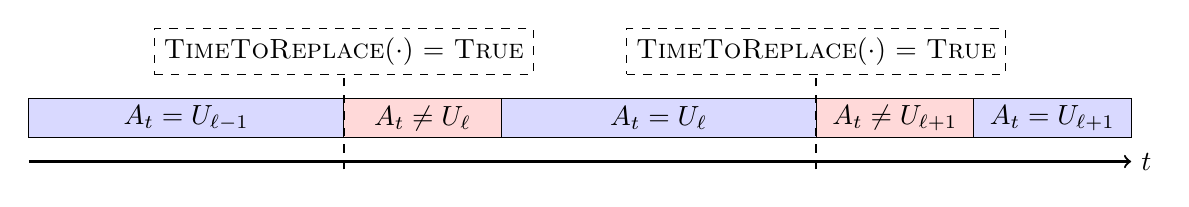
\begin{tikzpicture}[xscale=1, yscale=1]
    
    % timeline
    \draw[thick, ->] (0,0) -- (14,0) node[right] {\(t\)};
    
    % epoch labels
    % \node at (4.2,1.2) {\(\ell\)};
    % \node at (11,1.2) {\(\ell\gets \ell+1\)};
    
    % block phase of ell
    \draw[fill=blue!15] (0,0.3) rectangle (4,0.8);
    \node at (2,0.55) {\(A_t=U_{\ell-1}\)};
    
    % Transition phase of ell
    \draw[fill=red!15] (4,0.3) rectangle (6,0.8);
    \node at (5,0.55) {\(A_t\neq U_\ell\)};
    \draw[dashed, thick] (4,-0.1) -- (4,1.1);
    \node[draw, dashed] at (4,1.4) {\textsc{TimeToReplace}(\(\cdot\)) = \textsc{True}};
    
    % block phase of ell
    \draw[fill=blue!15] (6,0.3) rectangle (10,0.8);
    \node at (8,0.55) {\(A_t=U_{\ell}\)};
    
    % Transition phase of ell+1
    \draw[fill=red!15] (10,0.3) rectangle (12,0.8);
    \node at (11,0.55) {\(A_t\neq U_{\ell+1}\)};
    \draw[dashed, thick] (10,-0.1) -- (10,1.1);
    \node[draw, dashed] at (10,1.4) {\textsc{TimeToReplace}(\(\cdot\)) = \textsc{True}};
    
    % block phase of ell+1
    \draw[fill=blue!15] (12,0.3) rectangle (14,0.8);
    \node at (13,0.55) {\(A_t=U_{\ell+1}\)};
    
    \end{tikzpicture}
    \caption{Timeline of Algorithm \ref{alg:Optimistic-Hire}}
    \label{fig:intro-timeline}
\end{figure}

\vspace{-.2in}

This replacement rule also induces a useful cyclic structure on the timeline of the algorithm, shown in Figure~\ref{fig:intro-timeline}. Each cycle begins when \TimeToReplace(\(\cdot\)) returns True and a new target workforce \(U_\ell\) is selected. The workforce then passes through a transition phase, highlighted in red, during which the active workforce differs from \(U_\ell\) because the requested replacements have not yet fully completed. During this phase, the firm may operate with intermediate workforces. Once the replacements are realized, the algorithm enters a phase, highlighted in blue, in which the active workforce equals \(U_\ell\). The policy remains in this phase until the observation threshold in equation \eqref{eq:block-threshold} is met, at which point a new target workforce \(U_{\ell+1}\) is chosen and the cycle repeats. It is worth noting that in some cycles either phase may be empty. 

In each cycle, there is a phase during which the firm may need to operate with intermediate workforces. The composition of these workforces depends on how incoming and outgoing workers are paired.

\vspace{-.1in}
\subsection{Pairing Step}
Once a target workforce \(U_{\ell}\) has been chosen, the policy must convert it into concrete replacement requests. Given a target workforce \(U_{\ell}\) and an active workforce \(A_t\), we use a simple \emph{rank-matching} rule designed to make intermediate workforces less fragile during the transition. The key idea is the following bijection.

Let \(|\cdot|\) denote cardinality and \((i_1,\dots,i_r)\) the elements of \(A_{t}\setminus U_\ell\), with \(r := |A_{t}\setminus U_\ell| = |U_\ell\setminus A_{t}|\) ordered by their lower confidence bounds, i.e., 
\[
\LCB_{i_1}(t) \ge \LCB_{i_2}(t) \ge \cdots \ge \LCB_{i_r}(t).
\]
Similarly, let \((j_1,\dots,j_r)\) denote the elements of \(U_\ell\setminus A_{t}\), ordered so that
\[
\LCB_{j_1}(t) \ge \LCB_{j_2}(t) \ge \cdots \ge \LCB_{j_r}(t).
\]
We define the \emph{rank-matching} replacement bijection \(\pi^{\mathrm R}\) by matching workers according to their ranks, i.e., 
\begin{equation}\label{eq:rm-bijection}
    \pi^{\mathrm R}(i_s) = j_s, \qquad s=1,\dots,r.
\end{equation}
That is, workers to be removed and workers to be added are paired according to their relative lower-confidence rankings. The subroutine \ConstructPairing(\(\cdot\)) constructs this pairing between the target and active workforce:

\begin{algorithm}
    \caption{ConstructPairing}
    \label{alg:ConstructPairing}
    \begin{algorithmic}[1]
        \Require Current active workforce \(A_t\)
        \Require Target workforce \(U_{\ell}\)
        \Require Current count vector \(\mathbf{n}_t=(T_1(t),\dots,T_k(t))\)
        \Require Current empirical mean vector \(\boldsymbol{\mu}_t=(\bar{\mu}_1(t),\dots,\bar{\mu}_k(t))\)
        \State Compute \(\LCB_i(t)\) for all workers in the active workforce \(A_t\) and target workforce \(U_{\ell}\).
        \State Use LCBs to construct the rank-matching bijection \(R_t = \{  (i,\pi^{\mathrm{R}}(i)) : i \in  A_{t}\setminus U_{\ell}  \}\).
        \State \Return  \(R_t\).
    \end{algorithmic}
\end{algorithm}
Because replacements are completed after heterogeneous delays, the pairing step affects the sequence of intermediate workforces encountered during the transition. The rank-matching bijection is appealing because it satisfies several min--max properties with respect to a surrogate measure of transition regret. Those results are formalized in Appendix \ref{sec:bijection_analysis}. However, the main regret rate derive in Theorem \ref{thm:main} and Theorem \ref{thm:delta-main} hold for any pairing choice.

\subsection{Selection Rule}
We now turn to the second core component of the algorithm: the selection rule \ChooseTarget(\(\cdot\)), which determines the target workforce \(U_\ell\). A natural starting point is an optimism-based rule that selects the subset with the largest aggregate upper confidence bound. In our setting, however, replacement costs and a known planning horizon \(T\) require a refinement: near the end of the horizon, the remaining time may be too short for a replacement to recover its cost unless the potential improvement is sufficiently large. The subroutine \ChooseTarget(\(\cdot\)) incorporates this horizon-aware replacement criterion into an otherwise optimistic selection rule.

\begin{algorithm}
    \caption{ChooseTarget}
    \label{alg:ChooseTarget}
    \begin{algorithmic}[1]
        \Require Current active workforce \(A_t\)
        \Require Current count vector \(\mathbf{n}_t=(T_1(t),\dots,T_k(t))\)
        \Require Current empirical mean vector \(\boldsymbol{\mu}_t=(\bar{\mu}_1(t),\dots,\bar{\mu}_k(t))\)
        \State \Return Target workforce \(U\) which solves the optimization problem:
        \begin{align}\label{eq:opt}
            \max_{U} \quad & \sum_{i\in U}\UCB_i(t)\\
            \text{subject to}\quad &\sum_{i\in A_t\setminus U}\delta_{i,\pi^\mathrm{R}(i)}(t)\geq c\cdot \frac{| A_t\setminus U|}{T-t}
        \end{align}
    \end{algorithmic}
\end{algorithm}
The objective in Algorithm~\ref{alg:ChooseTarget} is optimistic, favoring target workforces with large upper-confidence values. The constraint tempers this optimism by requiring that the new workforce can plausibly recover its replacement cost over the remaining horizon. If this horizon-aware constraint is dropped, the optimization reduces to the unconstrained optimistic rule that simply selects the \(m\) workers with the largest UCB values. This unconstrained top-\(m\) UCB target is the ``unscreened'' variant used in the ablation study of Appendix~\ref{sec:oh-ablations}.

\begin{remark}[Computation of \textsc{ChooseTarget}]
    Since target selection is no longer a constrained optimization problem, it can no longer be solved greedily. Our approach proceeds as follows. For any fixed number \(r\) of replacements, the entering workers are given by the \(r\) inactive workers with the largest UCB values, so the only remaining decision is which \(r\) active workers to remove. This reduces \ChooseTarget to a cardinality-constrained knapsack problem over the active workforce. In Appendix \ref{sec:comp_of_selection_rule}, we develop an exact frontier-based dynamic program for this problem. Its runtime is polynomial in \(m\) and in the size of the maintained Pareto frontier, which in our simulations never exceeded 15 when \(m=100\). We discuss the practical implications of this observation in Section~\ref{numerical}.
\end{remark}

\section{Theoretical Performance Guarantee}
\label{theoretical}
We now turn to the performance implications of this approach. The following results show that adapting to delayed actions need not come at the expense of learning efficiency. Before establishing our main result, we provide a lower bound for combinatorial semi-bandits with delayed actions and costly replacements.

\begin{proposition} [Minimax lower bound]
\label{888}
Consider the stochastic delayed-replacement bandit model of Section~\ref{formulation}, with bounded rewards, \(m\) identical positions, and nonnegative-integer-valued delays. For any \(m\) and \(k\), and any horizon \(T > 0\), there exists an instance in this model class such that the regret of any algorithm is
\begin{equation*}
    \Regret(T) \geq \min \left\{\Omega\left(\sqrt{mkT}\right), \Omega\left(mT\right) \right\}.
\end{equation*}
\end{proposition}

The proof appears in Appendix \ref{sec:lower_bounds}. We now present our main theoretical result. When equipped with a suitable choice of the parameter \(\gamma\), our hiring policy achieves the same dominant \(\sqrt{T}\)-dependence as the lower bound in Proposition \ref{888}, up to logarithmic factors and lower-order friction terms. Delays and replacement costs enter through additive terms that can be controlled via \(\gamma\), which governs how aggressively the policy is permitted to adjust the workforce. 

\begin{theorem}[Instance-independent regret bound]\label{thm:main}
    Under the stochastic delayed-replacement model of Section~\ref{formulation}, assume rewards are bounded, the firm staffs \(m\) identical positions, delays are nonnegative integer-valued with \(\mathbb E[\omega_{i,j}^{(t)}]\le \bar{\omega}\), and the horizon \(T\) is known. Then there exist universal constants \(C_1, C_2, C_3>0\) independent of \((k,m,T,c,\bar{\omega})\) and \(\gamma\) such that for all \(k\ge 2\),
    \begin{eqnarray}
    \label{099}
        \Regret(T) &\le&  C_1 \sqrt{m(k-m)T\log T} 
         + C_2(k-m)\sqrt{\gamma \polylog(T)} \\
        &&\qquad\qquad\qquad\qquad + C_3 k\left(\gamma + (\bar{\omega}+c)m\right)
        + (\bar{\omega}+c)m\sqrt{\frac{kT}{\gamma}}
        \nonumber
    \end{eqnarray}
    Additionally, when \(\gamma = (\bar{\omega}+c)^2m\), there are different constants \(C_4, C_5\), independent of the problem parameters, such that
  \begin{eqnarray}
      \Regret(T) \leq C_4 \sqrt{mkT\log T} 
        +\; C_5km(c+\bar{\omega})^2\sqrt{ \polylog(T)}.
        \label{088}
        \end{eqnarray}
    The exact constants are given in Appendix \ref{sec:thm-all-constants}.
\end{theorem}

{\bf Explanation of regret.} This simplified bound has four distinct contributions that can be interpreted as follows. The term \(C_1 \sqrt{mkT\log T}\) has the same form as in frictionless models. It represents the intrinsic statistical difficulty of learning which workers perform well, independent of the operational constraints. The lower-order term, \(C_2\,(k-m)\sqrt{\gamma \polylog(T)}\), captures the additional learning cost induced by limiting the rate of replacements. Increasing the parameter \(\gamma\) lengthens the periods over which the workforce configuration is held fixed, reducing the frequency of updates but slowing the rate at which suboptimal workers can be identified and replaced. As a result, the learning regret grows with \(\sqrt{\gamma}\) and scales linearly with the number of suboptimal workers, \(k-m\). The remaining dependence on the horizon \(T\) enters only through polylogarithmic factors. The third term \(C_3\,k\left(\gamma + (\bar{\omega}+c)m\right)\), 
represents a horizon-independent ``start-up'' or ``burn-in'' cost that is standard in bandit learning algorithms. To make statistically meaningful decisions, the algorithm must obtain at least one observation from each worker; otherwise, it cannot distinguish unobserved workers from potentially optimal ones. 
% In the presence of execution delays and replacement costs, acquiring even a single observation from a worker may incur a delay of up to \(\bar{\omega}\) periods and a replacement cost of \(c\). Since the algorithm must obtain at least one observation from each of the \(k\) workers, this requirement alone induces an unavoidable cost proportional to \(k(\bar{\omega}+c)\). For comparison, related algorithms in settings with instantaneous actions and no replacement costs, such as \cite{kveton2014matroid}, incur a corresponding start-up cost of order \(km\). 
The remaining term, \((\bar{\omega}+c)\,m\sqrt{{kT}/{\gamma}}\), isolates the penalty of delayed actions and replacement costs over time. It scales like \(\sqrt{T}\) and decreases in \(\gamma\). More conservative updates (larger \(\gamma\)) reduce the cumulative impact of frictions by limiting how often the workforce is changed. In contrast, smaller \(\gamma\) makes the policy more agile but amplifies this friction-driven component. 

The second part of Theorem \ref{thm:main}, which chooses \(\gamma = (\bar{\omega}+c)^2 m\), shows that this trade-off can be resolved in favor of learning. Once \(\gamma\) is chosen large enough relative to the magnitude of the frictions, the \((\bar{\omega}+c)m\sqrt{kT/\gamma}\) term becomes \(\tilde{O}(\sqrt{kmT}\,)\), the same order as the frictionless lower bound, and the leading \(\sqrt{T}\) term of the bound becomes independent of \(c\) and \(\bar{\omega}\).

{\bf High replacement cost.} In the bound in Theorem \ref{thm:main}, the replacement cost $c$ is a constant and independent of $T$. In situations where replacement cost is relatively high, we can model $c$ as 
a function of $T$, e.g., $c=\Theta(\log T)$ or $c=\Theta(T^{1/4})$. From (\ref{088}), it is seen that as long as the replacement cost grows at rate  
$$c\;\le \; O\big((T/(mk))^{1/4}-\bar{\omega}\big)^+,$$ 
where $x^+=\max\{x, 0\}$ for any real $x$, then the regret of \textsc{OH} policy will be $\tilde O(\sqrt{mkT})$. 

{\bf Instance-dependent regret.} Along with our main result, we prove an asymptotic instance-dependent bound on the regret. Before presenting the result, we introduce the concept of consistent policies so that we may state the accompanying lower bound. 

We call a policy \emph{consistent} (sometimes ``uniformly good'') if, for all replacement bandit policies, \(\limsup_{T\to \infty}\Regret(T)/T^\alpha=0\) for all \(\alpha>0\) \citep{lattimore2020bandit}. In this setting, the following lower bound holds. 

\begin{proposition}[Instance-dependent regret lower bound]\label{prop:asymptoptic-lower}
    Under the stochastic delayed-replacement model of Section~\ref{formulation}, assume the firm staffs \(m\) identical positions and rewards are Bernoulli. Fix any \(\Delta \in (0,1/2)\), and consider an instance with means
    \[\mu_i =\begin{cases}
        1/2, & i = 1,\dots,m,\\
        1/2-\Delta, & i = m+1,\dots,k.
    \end{cases}\]
    Then any consistent algorithm satisfies
    \[
        \liminf_{T\to\infty}\frac{\Regret(T)}{\log T}\geq \Omega\left(\frac{k-m}{\Delta}\right).
    \]
\end{proposition}
This proposition is proved in Appendix \ref{sec:lower_bounds}. We then have the upper bound for \textsc{Optimistic-Hire}. As before, the bound with all constants is available in Appendix \ref{sec:delta-all-constants}.
\begin{theorem}[Instance-dependent regret bound]\label{thm:delta-main}
    Under the stochastic delayed-replacement model of Section~\ref{formulation}, assume rewards are bounded, the firm staffs \(m\) identical positions, delays are nonnegative integer-valued with \(\mathbb E[\omega_{i,j}^{(t)}]\le \bar{\omega}\), and the horizon \(T\) is known. Suppose further that there are \(m\) unique best arms (i.e., \(\mu_1\geq \cdots \geq \mu_m >\mu_{m+1}\geq \mu_k\)). Define \(\Delta_{i,j}:=\mu_i-\mu_j\) to be the optimality gap. Then there exist constants \(C_1,C_2,C_3\), and \(C_4\) such that when \(T>k\),
    \begin{align*}
        \Regret(T)&\leq C_1\sum_{j>m}\frac{1}{\Delta_{m,j}} \left( \log T+(\bar{\omega}+c)m\sqrt{\frac{k\log T}{\gamma }}\right)\\
        &\quad +~ C_2\sum_{j>m} \left[\sqrt{\gamma \log T\cdot \polylog\left(\frac{\Delta_{1,j}}{\Delta_{m,j}}\right)}+c\log\left(\frac{c}{\Delta_{m,j}}\right)\right]\\
        & \quad + ~C_3\sum_{j>m} \Delta_{1,j} \left[(\gamma + 1) + \frac{m}{T}\right]\\
        &\quad +~C_4(\bar{\omega}+c)mk
    \end{align*}
    Additionally, when \(\gamma=(\bar{\omega}+c)m\), there are different constants \(C_5, C_6\), independent of the problem parameters, such that
    \begin{align*}
        \Regret(T)&\leq C_5\sum_{j>m}\left[\frac{\log T}{\Delta_{m,j}}+\left(\polylog\left(\frac{\Delta_{1,j}}{\Delta_{m,j}}\right)+\frac{1}{\Delta_{m,j}}\right)\sqrt{(\bar{\omega}+c)mk\log T}\right]\ \\
        &\quad +~ C_6\sum_{j>m} \left[c\log\left(\frac{c}{\Delta_{m,j}}\right)+m\Delta_{1,j} \left(\bar{\omega}+c + \frac{1}{T}\right)\right]
    \end{align*}
\end{theorem}
From this upper bound we can derive that the scaling of the instance-dependent bound is optimal.
\begin{corollary}
    Suppose that there are \(m\) unique best arms (i.e. \(\mu_1\geq \cdots \geq \mu_m >\mu_{m+1}\geq \mu_k\)).
    \[\limsup_{T\to\infty}\frac{\Regret(T)}{\log T}\leq \sum_{j>m}\frac{8}{\Delta_{m,j}}\]
    In particular, for \(\Delta:=\min_{i\leq m,j>m}\mu_i-\mu_j\),
    \[\limsup_{T\to\infty}\frac{\Regret(T)}{\log T}\in O\!\left(\frac{k-m}{\Delta}\right)\]
\end{corollary}

{\bf Practical choice of \(\gamma\).}
In practice, we recommend choosing \(\gamma\) by numerically minimizing the regret upper bound in Theorem \ref{thm:main} over the known parameters \((c, \bar{\omega}, k, m, T)\). These parameters are typically known to the decision maker, so this strategy is implementable in practice. In the numerical experiments of Section \ref{numerical}, we use this choice of parameter.


%\vspace{-.1in}

\section{Numerical Experiments}
\label{numerical}
This section presents numerical experiments designed to clarify what the proposed policy does well, what aspects of the model drive those gains, and what the experiments do and do not establish. We begin with a calibrated fulfillment-center-inspired benchmark. We then vary the staffing ratio, replacement delays, and replacement costs in the main text. Additional appendix experiments examine sensitivity to the tuning parameter \(\gamma\), the optimality-gap structure, the robustness of tuned-threshold heuristics, the tractability of the \ChooseTarget subproblem, and which parts of \textsc{Optimistic-Hire} contribute most to the performance gains.

\vspace{-.1in}

\subsection{Benchmarking}\label{numerical:benchmarks}
To evaluate the empirical performance of \textsc{Optimistic-Hire}, we simulate a stylized fulfillment setting with onboarding delays. The firm has access to a pool of \(k=150\) temporary workers and employs \(m=100\) workers in each period. This corresponds to a relatively tight labor regime in which a large share of the available worker pool is deployed in each period, as may arise when labor demand is high relative to available supply. For completeness, we also simulate a regime with greater labor slack (\(m=50\)). We assume the facility operates continuously (24 hours per day, 365 days per year). Time is discretized at the hourly level, reflecting the granularity at which productivity and labor allocation are typically tracked in fulfillment operations. This gives a maximum horizon of \(T=5 \cdot 365 \cdot 24\). 

When a new worker is hired, they must complete an onboarding process before becoming productive. We model onboarding as requiring a full 8-hour shift during which the worker generates no output. Moreover, the firm must pay the worker for this time. This assumption is consistent with warehouse training practices, where new hires undergo paid orientation and initial instruction before contributing to throughput. Operationally, this corresponds to a delay of \(8\) periods and an effective replacement cost proportional to 8 periods of worker pay, which we model as \(c=8\). Finally, we draw the intrinsic productivity of each worker uniformly between 0.3 and 0.7. 

The \textsc{Optimistic-Hire} parameter \(\gamma\) is chosen to numerically minimize the regret bound with all constants (see Appendix \ref{sec:thm-all-constants}) given the known parameter values \(c=8\), \(\bar{\omega}=8\), \(k=150\), \(m=100\), and \(T=5\) years. 

\begin{remark}[Computational Tractability]
    As discussed after Algorithm~\ref{alg:ChooseTarget}, the \ChooseTarget exact solver is a dynamic program whose complexity is polynomial in the size of its frontier. In our local Python implementation of the benchmark calibration \((k=150,m=100,T=43{,}800)\), a full five-year \textsc{Optimistic-Hire} simulation run takes about 5 seconds on average, the mean time per \ChooseTarget call is about 27 milliseconds, and the largest frontier we observed in the frontier-size study was 11 states. Appendix~\ref{sec:comp_of_selection_rule} provides the algorithmic details, and Figure~\ref{fig:frontier-size} shows that in the broader benchmark study the maintained frontier remained very small throughout. 
\end{remark}

{\bf Comparison policies.}
The setting most closely related to ours is the \(m\)-play bandit with replacement costs and instantaneous actions. Accordingly, we benchmark against the standard algorithm from this literature, \cite{agrawal1990switching}, which we denote AgrawalHedgeTeneketzis (\textsc{AHT}). The second benchmark algorithm we implement is the Optimistic Matroid Maximization algorithm (\textsc{OMM}) from \cite{kveton2014matroid}, which employs an optimism-based selection rule similar to ours and achieves \(O(\sqrt{kmT})\) regret in the absence of delays and replacement costs. This choice reflects the canonical regret-optimal approach for stochastic matroid bandits, a class that includes the \(m\)-play setting as a special case.

Because our setting involves delayed actions, both algorithms must be adapted before they can be implemented. First, the original algorithms prescribe workforce selections, whereas in our setting decisions are implemented through replacements. At each decision epoch, we query the algorithm for its desired workforce and then translate that workforce into a set of replacement requests. In the main benchmark, we use a random pairing for these delayed-action adaptations. Proposition \ref{lem:iid-rank-matching-E} suggests this should not materially weaken the expected regret. Second, the original algorithms assume instantaneous actions and therefore do not account for the feasibility constraints induced by delays. In particular, proposed replacements may violate the coherence constraints \eqref{eq:coherence-1}--\eqref{eq:coherence-2}, for example by attempting to remove or add a worker who is already involved in a pending replacement. To enforce feasibility, we discard any conflicting replacement requests. More sophisticated delay-aware adaptations may be possible, but they would require substantial modifications to the original policies. For \textsc{AHT}, it is not clear how to preserve its calendar-time-based update schedule without such modifications, since delayed replacements can prevent the requested workforce changes from being realized on schedule. For the other adapted policy \textsc{OMM}, our numerical results in Section \ref{numerical:cost} suggest that our adaptation \emph{improves} the polices performance. Because \textsc{OMM} is not designed to account for replacement costs, discarding some replacement decisions, and thus reducing the rate of replacements, improves its performance. 
Appendix~\ref{sec:oh-ablations} complements those external comparisons with internal ablations of \textsc{Optimistic-Hire}: adaptive versus fixed-calendar replacement timing, horizon-aware selection versus the unconstrained version of \ChooseTarget (namely the top-\(m\) UCB target), and rank-matching versus random pairing. In Section \ref{numerical:delayed}, we additionally compare \textsc{Optimistic-Hire} with the benchmark policies in the no-delay regime, where no delay-related adaptations are required and any performance differences therefore cannot be attributed to those modifications.

We also include several heuristics intended to reflect common employment practices. The first benchmark, denoted \textsc{TunedThreshold}(\(\tau\)), is a fixed-threshold screening policy. It retains each worker in the active workforce as long as that worker's empirical mean reward remains at least \(\tau\). Whenever a worker's empirical mean falls below this threshold, the policy replaces that worker with the available alternative having the highest empirical mean, treating unobserved workers as having infinite empirical mean. For each simulation instance, the threshold value \(\tau\) is selected in a preliminary calibration step by evaluating a grid of candidate thresholds with spacing \(0.05\) and choosing the best-performing value. The second is \textsc{SemiAnnualReview}. This policy reviews its active workforce every 6 months and requests replacements to achieve the empirically best-performing workforce. The last is \textsc{WorkTrial}. This policy is based on a guidance from Indeed, a leading job posting company \citep{indeed_job_trial}. The policy employs each worker for 1 hour, or for as short a tenure as possible (delays may cause this to be longer than 1 hour). It then selects the top \(2m\) workers by empirical mean. The firm employs the first \(m\) for 90 days, then replaces them with the second \(m\) for 90 days. This corresponds to a ``work trial.'' Afterward, the firm permanently retains the \(m\) best-performing workers.

{\bf Results.}
We evaluate performance using two metrics. The first is the cumulative regret, defined in \eqref{def:regret}. The second is the normalized loss,
\[
\mathrm{Normalized\ Loss}(T)
    := \frac{\Regret(T)}{T\,\mu(A^*)} \times 100\%,
\]
which measures regret as a fraction of the oracle benchmark's total reward over the same horizon.

We run the main benchmark on \(25\) independently generated instances, with worker means drawn uniformly from \([0.3,0.7]\). Figure~\ref{fig:benchmark} plots the mean trajectory for each policy, with shaded bands showing \(\pm 1\) standard deviation across runs.

\begin{figure}[t]
    \centering
    \begin{minipage}[t]{0.48\linewidth}
        \centering
        
\includegraphics[width=\linewidth]{paper-images/benchmark_cum_regret.png}
    \end{minipage}
    \hfill
    \begin{minipage}[t]{0.48\linewidth}
        \centering
        
\includegraphics[width=\linewidth]{paper-images/benchmark_normalized_loss.png}
    \end{minipage}

    \caption{Simulated performance of \textsc{Optimistic-Hire} compared with benchmarks when \(m=100\).}
    \label{fig:benchmark}
\end{figure}

The main message is that \textsc{Optimistic-Hire} provides the strongest overall performance among the policies and delayed-action adaptations tested here. Although some benchmark policies perform well over particular portions of the horizon, \textsc{Optimistic-Hire} is the only method that remains consistently near the frontier throughout and is best at the terminal five-year horizon. In particular, at five years it achieves the smallest cumulative regret and normalized loss among all policies tested.

% Figure \ref{fig:benchmark} also highlights the different exploration profiles of the benchmark policies. The policy \textsc{AHT} performs well early, but its regret continues to grow faster than that of \textsc{Optimistic-Hire}. This is consistent with the conservative structure of \textsc{AHT}: in each period it selects \(m-1\) workers greedily based on empirical means, which helps it assemble a reasonably good workforce quickly but limits its ability to continue learning. By contrast, \textsc{WorkTrial} and \textsc{SemiAnnualReview} flatten earlier, but at a higher regret level, suggesting that they spend too long exploring suboptimal workers before settling on a stable workforce. \textsc{Optimistic-Hire} achieves a better balance. Like \textsc{AHT}, it identifies a strong workforce relatively quickly, but it also preserves enough exploration to continue improving over time. As a result, it combines good short-run performance while still finding near-optimal workforces (as indicated by the nearly flat regret curves) in the medium and long run. It is worth noting that the parameter \(\gamma\) for \textsc{Optimistic-Hire} is tuned for the full five-year horizon. Even so, it remains competitive at one month, is already best by one year, and remains the leader for the rest of the horizon. 

% The magnitude of improvement is also meaningful. 
At five years, \textsc{Optimistic-Hire} reduces cumulative regret by about \(73\%\) relative to \textsc{AHT}, about \(88\%\) relative to \textsc{OMM}, and about \(48\%\) relative to \textsc{WorkTrial}. It is also the most stable policy across instances. Additionally, \textsc{Optimistic-Hire} reduces the variability of cumulative regret by about \(78\%\) relative to \textsc{AHT}, about \(79\%\) relative to \textsc{WorkTrial}, and about \(82\%\) relative to \textsc{OMM}. Thus, within this benchmark set, \textsc{Optimistic-Hire} not only achieves the best mean performance at the target horizon, but does so substantially more reliably across heterogeneous instances. Appendix \ref{sec:benchmark_tables} provides tables listing cumulative regret and normalized loss at horizons 1 month, 12 months, 3 years, and 5 years.

Appendix~\ref{sec:oh-ablations} helps separate which design choices drive these gains. In the benchmark calibration, replacing the adaptive count-based replacement rule by a fixed calendar schedule raises 12-month regret from \(6{,}462\) to \(7{,}785\) and five-year regret from \(11{,}621\) to \(16{,}711\) in a 20-run ablation. Replacing the horizon-aware selection rule by the unconstrained version of \ChooseTarget, namely the top-\(m\) UCB target, also worsens performance, though more modestly, increasing 12-month regret to \(6{,}765\) and five-year regret to \(12{,}161\). By contrast, replacing rank matching with random pairing has no visible effect in this low-cost i.i.d.\ benchmark. This is the behavior we would expect in light of Proposition \ref{lem:iid-rank-matching-E}. We therefore interpret the main benchmark as evidence primarily for the replacement-and-selection architecture of \textsc{Optimistic-Hire}, with the adaptive replacement rule as the dominant driver and horizon-aware selection as a useful secondary refinement in this regime.

Figure~\ref{fig:benchmark_50_150} reports results for the lower-utilization regime with \(m=50\), so that a smaller fraction of the worker pool is employed in each period. This provides a robustness check with respect to the staffing ratio. The qualitative pattern is unchanged: \textsc{Optimistic-Hire} again performs best over the medium and long horizons, while remaining competitive early. While \textsc{TunedThreshold} performs best in the short run, it relies on tuning parameters that depend on unknown problem characteristics, most notably the optimality gaps. Accordingly, it should be viewed as a best-case benchmark rather than as a deployable policy. Appendix~\ref{sec:threshold-robustness} shows that its performance can deteriorate substantially under even mild perturbations of the underlying unknown problem parameters.

\begin{figure}[t]
    \centering
    \begin{minipage}[t]{0.48\linewidth}
        \centering
        
\includegraphics[width=\linewidth]{paper-images/benchmark_cum_regret_50_150.png}
    \end{minipage}
    \hfill
    \begin{minipage}[t]{0.48\linewidth}
        \centering
        
\includegraphics[width=\linewidth]{paper-images/benchmark_normalized_loss_50_150.png}
    \end{minipage}

    \caption{Simulated performance of \textsc{Optimistic-Hire} compared with benchmarks when \(m=50\).}
    \label{fig:benchmark_50_150}
\end{figure}


\vspace{-.1in}

\subsection{Effects of Delayed Replacements}\label{numerical:delayed}
In Figure~\ref{fig:sweep_delay}, we examine the effect of delayed replacements by varying the maximum delay parameter \(\omega_{\max}\) of the uniform delay distribution.
% and the delay-generation process. 
In the case study described in Section~\ref{numerical:benchmarks}, the values of \(\omega_{\max}\) correspond to a zero-delay case (requests may be realized in the same period before rewards are drawn), a maximum delay of 24 hours (one day), and a maximum delay of 72 hours (three days). We implement a stochastic delay-generation process in which each \(\omega^{(t)}_{i,j}\) is drawn uniformly from \(\{0,\dots,\omega_{\max}\}\).


\begin{figure}[H]
    \centering
    \begin{minipage}{0.3\linewidth}
        \centering
        \includegraphics[width=\linewidth]{paper-images/benchmark_delay_stochastic_omega_0.png}
    \end{minipage}
    \hfill
    \begin{minipage}{0.3\linewidth}
        \centering
        
\includegraphics[width=\linewidth]{paper-images/benchmark_delay_stochastic_omega_24.png}
    \end{minipage}
    \hfill
    \begin{minipage}{0.3\linewidth}
        \centering
        \includegraphics[width=\linewidth]{paper-images/benchmark_delay_stochastic_omega_72.png}
    \end{minipage}
    \caption{Simulated performance of \textsc{AHT}, \textsc{OMM}, and \textsc{Optimistic-Hire} under several delay settings.}
    \label{fig:sweep_delay}
    \vspace{-.15in}
\end{figure}

Figure~\ref{fig:sweep_delay} yields three main observations. First, \textsc{Optimistic-Hire} outperforms \textsc{AHT} even in the zero-delay regime \((\omega_{\max}=0)\). In this case in which accepted replacements can be realized in the same environment step before period-\(t\) rewards are generated, so no delay-specific feasibility frictions remain beyond the replacement-cost structure inherited from \cite{agrawal1990switching}. The performance gap therefore cannot be attributed solely to the way \textsc{AHT} is modified for delayed replacements, and instead suggests that \textsc{Optimistic-Hire} more effectively balances exploration and replacement timing even when requests can be implemented immediately.

Second, the variability of regret for \textsc{AHT} increases with the delay length, whereas the variability of \textsc{Optimistic-Hire} remains comparatively stable. This reflects the deterministic calendar-time update schedule used by \textsc{AHT}: when delays are long, realized replacements can lag behind the prescribed schedule, so the active workforce and the amount of information collected at an update epoch may differ from what the policy anticipates. This points to the adaptive replacement rule in \textsc{Optimistic-Hire} as an important source of robustness, since it responds to realized observations rather than calendar time alone.

Finally, the regret of \textsc{OMM} \emph{decreases} as delays increase. The reason is that \textsc{OMM} initiates too many replacements, which generates excessive replacement costs. Larger delays cause more of these intended replacements to be discarded, effectively regularizing the policy's replacement frequency. This highlights an important operational caution: delays are not always harmful. What matters operationally is the replacement rate. If the firm is already replacing at a near-optimal rate, reducing delays improves performance. But if the firm is already replacing too frequently, reducing delays may counterintuitively \emph{worsen} performance.


\subsection{Effects of Replacement Cost Magnitude}\label{numerical:cost}
In Figure~\ref{fig:sweep_c}, we examine the effect of replacement costs on \textsc{AHT}, \textsc{OMM}, and \textsc{Optimistic-Hire} under the same setup as Section~\ref{numerical:benchmarks}, with \(k=150\), \(m=100\), and \(\bar{\omega}=8\). The first plot shows cumulative regret when there are no costs \((c=0)\). In this setting, \textsc{Optimistic-Hire} performs better than \textsc{AHT} at the 5 year horizon with significantly lower variance. Notably, it also recovers performance competitive with \textsc{OMM}. When costs are larger, with \(c\in \{24, 72\}\), \textsc{Optimistic-Hire} performs substantially better than both other policies. This is consistent with the role of the horizon-aware screening constraint in \ChooseTarget: as replacements become more expensive, ruling out late or weakly justified replacements becomes more valuable.

\begin{figure}[H]
    \centering
    \begin{minipage}{0.3\linewidth}
        \centering
        
\includegraphics[width=\linewidth]{paper-images/benchmark_cost_0.png}
    \end{minipage}
    \hfill
    \begin{minipage}{0.3\linewidth}
        \centering
        
\includegraphics[width=\linewidth]{paper-images/benchmark_cost_24.png}
    \end{minipage}
    \hfill
    \begin{minipage}{0.3\linewidth}
        \centering
        \includegraphics[width=\linewidth]{paper-images/benchmark_cost_72.png}
    \end{minipage}
    \caption{Simulated performance of \textsc{AHT}, \textsc{OMM}, and \textsc{Optimistic-Hire} under several cost settings.}
    \label{fig:sweep_c}
    \vspace{-.15in}
\end{figure}

Taken together, the numerical results suggest three distinct mechanisms behind the performance of \textsc{Optimistic-Hire}. The no-delay comparison indicates that the optimistic, horizon-aware selection rule is already competitive even before delays matter. The delay study then isolates the benefit of the adaptive replacement schedule, which appears to stabilize performance when realized completion times vary substantially. Finally, the cost study shows why screening replacements through the remaining-horizon constraint matters: when workforce changes are expensive, avoiding marginal late-horizon replacements becomes increasingly valuable. Appendix~\ref{sec:oh-ablations} makes this decomposition more explicit. In the benchmark calibration, fixed-calendar replacement timing materially worsens both short- and long-run performance, replacing the horizon-aware selection rule by the unconstrained version of \ChooseTarget (the top-\(m\) UCB target) also increases regret but by a much smaller amount. The high-cost stress test then shows that the value of horizon-aware selection becomes much larger once late replacements are expensive. This pattern is consistent with the intended role of the screen as a finite-horizon cost-benefit filter. In the appendix we provide additional experiments including \(\gamma\)-sensitivity experiments that show that the bound-based choice of \(\gamma\) is empirically reasonable and that the best replacement frequency shifts with the gap structure.

\section{Concluding Remarks}\label{sec:conclusion}
This paper studies sequential hiring decisions in contingent labor environments. We formulate hiring as a bandit problem with replacement costs and worker-availability uncertainty through an action-delay structure. We propose a learning-based hiring policy centered on adaptive replacement timing and horizon-aware selection, together with a pairing step for managing intermediate workforces. We show that the proposed algorithm attains a regret bound whose leading-order dependence on \(T\) matches the lower bound up to logarithmic and lower-order friction terms. In particular, when replacement frequency is controlled appropriately, the policy achieves cumulative regret with the same \(\tilde{O}(\sqrt{kmT})\) dependence as the lower bound for combinatorial delayed and costly replacement. When replacement costs are large and grow with the time horizon \(T\), the algorithm parameter can be chosen to minimize total regret. Our numerical experiments are supportive: across the calibrated settings and delayed-action benchmark adaptations we study, the proposed policy compares favorably with both classical algorithms for instantaneous actions with costly adjustments and several operationally motivated heuristics. The additional ablations indicate that the adaptive replacement rule and horizon-aware selection components drive most of those gains in our benchmark calibration, while the pairing rule is best viewed as a complementary refinement for managing intermediate workforces under less favorable delay realizations.

The model developed in this paper is most applicable when the pool of potential workers---for example, recommendations provided by a platform---is moderate, or when the firm has at least some initial performance data for most workers in a large pool. In the first case, the firm can realistically test all potential workers over the planning horizon. In the second, the firm begins with finite UCB and LCB values for each worker, so \textsc{OH} need not explore the entire pool and can instead focus on a promising subset. By contrast, when the worker pool is very large or effectively unbounded and the firm has little or no initial data on most workers, exhaustively testing workers over the horizon is not practical, and a different modeling approach is needed. One possible direction is to adapt methods such as those in \cite{wang2008algorithms}, which first identify a finite subset that contains a sufficiently good arm with high probability and then apply a finite-armed bandit algorithm to that restricted set. Another direction is to use a contextual bandit model, in which each worker has observable features and productivity depends on those features. The simplest examples are linear and generalized linear bandit models, where expected reward is parameterized as a function of observed covariates and learning reduces to estimation of the underlying coefficients.

The model studied here also abstracts from several important features of real labor markets. In particular, we do not model endogenous worker behavior such as voluntary quitting, strategic acceptance or rejection of assignments, or exit from the labor market. We also assume stationary worker productivity, identical positions, exogenous delays, and a known planning horizon in the analyzed policy. These assumptions are appropriate for a first stylized model of learning-based contingent hiring, but they also define the scope of the conclusions that can be drawn. Incorporating richer worker-side behavior or endogenous supply would fundamentally alter the information structure faced by the firm and would likely require tools from dynamic games, mechanism design, or learning in environments with endogenous participation.


% NOTE: Use the Code and Data Disclosure section to provide instructions for where your code and data, along with README file, can be found. If the paper received an exemption, then state the reason the exemption was granted.

\section{Code and Data Disclosure}\label{sec:code-data-disclosure}
The code used in this paper is available at \url{https://github.com/leechr001/hiring-bandit}. The repository includes the simulation environment, implementations of all policies reported in the paper, and scripts to reproduce the figures, tables, and internal ablations reported in the appendices. 


% {\color{red} Please clean up the references. They are now not professionally done -- check consistence on capitalizing initials of journal/conference titles}
\bibliographystyle{informs2014} % outcomment this and next line in Case 1
\bibliography{hiring-bandit} % if more than one, comma separated


%\THEEndNotes
%\begingroup \parindent 0pt \parskip 0.0ex \def\enotesize{\normalsize} \theendnotes \endgroup

% Appendix here
% Options are (1) APPENDIX (with or without general title) or
%             (2) APPENDICES (if it has more than one unrelated sections)
% Outcomment the appropriate case if necessary
%
% \begin{APPENDIX}{<Title of the Appendix>}
% \end{APPENDIX}
%
%   or
%

\newpage
%\setcounter{page}{1}
%\newgeometry{left=1cm,bottom=1cm}
\begin{APPENDICES}


\noindent {\Large Appendices: Technical Proofs}
%\end{APPENDICES}{}
%\renewcommand{\textwidth}{18cm}
%\renewcommand{\baselinestretch}{0.72}

%\geometry{a4paper,scale=0.8}
    
%\vspace{0.3cm}
%\section{Technical Proofs}\label{app:proof}
\vspace{.1in}

% {\color{red} change to format to replace ``:" after "Appendix A" by ``." (to make it consistent with earlier sections)}
% %\begin{APPENDICES}

\section{Statement of the Main Theorem With Exact Constants}\label{sec:thm-all-constants}
Let \(k\) denote the number of arms, \(m\) the size of each solution, and \(\gamma>0\) a policy parameter. Then the expected regret of Algorithm 1 over \(T\) periods satisfies
\begin{eqnarray*}
    \Regret(T) &\leq& 5\sqrt{m(k-m)T\log T}\\
    &&+\;(c+1)(k-m) +(k-m)c\log\left(\frac{cmT}{(k-m)\log T}\right)\\
    &&+ k(\gamma + 1) + \frac{4mk}{T}\\
    &&+2(k-m)\sqrt{\gamma \cdot 4\log T}
    \left(1+\frac{1}{2}\log\!\left(\frac{mT}{(k-m)\log T}\right)\right)\\
    &&+\;(\bar{\omega}+c) m\sqrt{\frac{kT}{\gamma}} + (\bar{\omega}+c)mk.
\end{eqnarray*}

\section{Language, Notation, and Structure for Proofs}
To streamline the presentation of the proofs, we describe the workforce-selection problem using the standard language of bandit algorithms. In this formulation, workers are treated as ``arms,'' the \(m\)-worker roster corresponds to a ``solution,'' observed productivity is interpreted as a ``reward,'' and employing a worker is viewed as ``playing an arm.'' We also introduce structural notation describing the algorithm's control flow, decision instants, and target solutions, which will be used consistently throughout the analysis.

Each time Algorithm~\ref{alg:Optimistic-Hire} initiates replacements, the counter \(\ell\) increases. This counter also indexes the sequence of target solutions \(U_{\ell}\). Accordingly, we refer to each \(\ell = 1,2,\dots\) as an epoch. The target solution \(U_\ell\) associated with epoch \(\ell\) is computed in the first period of that epoch. We call this initial time the \emph{decision instant} and denote it by
\begin{equation}\label{eq:c-def}
    d_\ell := \text{the first period of epoch \(\ell\)}.
\end{equation}
The algorithm may not be able to play \(U_\ell\) immediately because of arm unavailability. Instead, it gradually transitions toward \(U_\ell\) and commits to playing it once all arms in \(U_\ell\) are available. We denote this first play time by the \emph{play instant},
\begin{equation}\label{p-def}
    p_\ell := \text{the first period in which \(U_\ell\) is available}.
\end{equation}
This naturally partitions each epoch into two phases:
\[
    \mathcal{T}_\ell = \{ t : d_\ell \le t < p_\ell \},
    \quad
    \mathcal{B}_\ell = \{ t : p_\ell \le t < d_{\ell+1} \}.
\]
We call the first phase the \emph{transition phase}, since the active set moves from the previous target solution to the new one. We refer to the second phase as the \emph{block phase}, since it plays a role analogous to the blocks in block-based algorithms. Unlike in those algorithms, however, the length of our block phases is adaptive: the length of \(\mathcal{B}_{\ell}\) depends on the realized delays. For example, it is possible that \(\mathcal{B}_\ell = \emptyset\) if the realized delays are sufficiently long. Likewise, it is possible that \(\mathcal{T}_\ell = \emptyset\) if \(U_\ell\) is available immediately at \(d_\ell\). Figure~\ref{fig:timeline} illustrates these intervals.

A crucial feature of this setup is that although each epoch is structured around a single target solution \(U_{\ell}\), the actual plays of an arm \(j \in U_\ell\) need not occur exclusively within that epoch. Conversely, during epoch \(\ell\), arms from \(U_{\ell-1}\) may still be played regardless of whether they belong to \(U_\ell\). For convenience, we define
\[
    \epoch(t) := \text{the unique \(\ell\) such that \(t \in \mathcal{T}_\ell \cup \mathcal{B}_\ell\)},
\]
and let \(L := \epoch(T)\) denote the index of the last epoch before horizon \(T\).

\begin{figure}[t] 
    \centering
    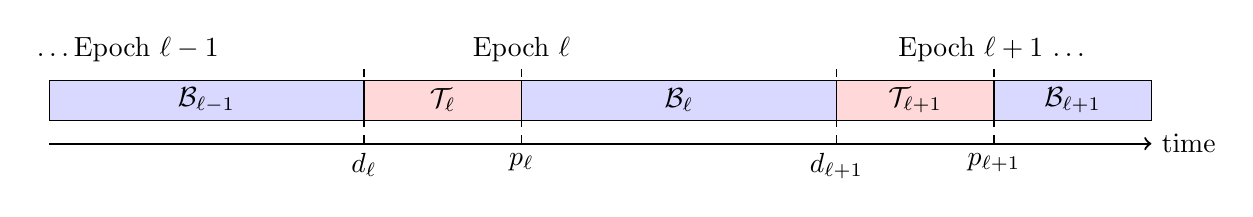
\begin{tikzpicture}[xscale=1, yscale=1]
    
    % timeline
    \draw[thick, ->] (0,0) -- (14,0) node[right] {time};
    
    % epoch labels
    \node at (1,1.2) {\dots Epoch \(\ell-1\)};
    \node at (6,1.2) {Epoch \(\ell\)};
    \node at (12,1.2) {Epoch \(\ell+1\) \dots};
    
    % block phase of ell
    \draw[fill=blue!15] (0,0.3) rectangle (4,0.8);
    \node at (2,0.55) {\(\mathcal{B}_{\ell-1}\)};
    
    % Transition phase of ell
    \draw[fill=red!15] (4,0.3) rectangle (6,0.8);
    \node at (5,0.55) {\(\mathcal{T}_\ell\)};
    
    % block phase of ell
    \draw[fill=blue!15] (6,0.3) rectangle (10,0.8);
    \node at (8,0.55) {\(\mathcal{B}_{\ell}\)};
    
    % Transition phase of ell+1
    \draw[fill=red!15] (10,0.3) rectangle (12,0.8);
    \node at (11,0.55) {\(\mathcal{T}_{\ell+1}\)};
    
    % block phase of ell+1
    \draw[fill=blue!15] (12,0.3) rectangle (14,0.8);
    \node at (13,0.55) {\(\mathcal{B}_{\ell+1}\)};
    
    % Mark c(l)
    \draw[dashed] (4,0) -- (4,1);
    \node[below] at (4,0) {\(d_\ell\)};
    
    % Mark p(l)
    \draw[dashed] (6,0) -- (6,1);
    \node[below] at (6,0) {\(p_{\ell}\)};
    
    % Mark c(l+1)
    \draw[dashed] (10,0) -- (10,1);
    \node[below] at (10,0) {\(d_{\ell+1}\)};
    
    % Mark p(l+1)
    \draw[dashed] (12,0) -- (12,1);
    \node[below] at (12,0) {\(p_{\ell+1}\)};
    
    \end{tikzpicture}
    \caption{Timeline of consecutive epochs and their phases.}
    \label{fig:timeline}
\end{figure}


\vspace{-.1in}

\section{Proof of the Regret Bound}\label{sec:proof-outline}
In this section, we sketch the main argument underlying the regret bound and highlight the key properties on which the analysis depends. Proofs of the supporting lemmas are given in the subsequent sections.

The regret naturally consists of two components. Let \(S_T\) denote the \emph{sampling regret}, corresponding to the regret incurred from selecting suboptimal workers, and let \(J_T\) denote the \emph{replacement cost}. Then
\[
\Regret(T) = S_T + J_T.
\]

%\subsubsection
{\bf Bounding replacement costs.}
The main difficulty in controlling replacement-cost regret is that epoch lengths are both \emph{endogenous} and \emph{history dependent}: the duration of an epoch depends on the realized delays and on the number of samples accumulated by the least-observed arm. Consequently, epoch lengths are coupled to both the learning trajectory and the unknown delay process. Moreover, the block thresholds \(N(\ell)\) need not be monotone in the epoch index \(\ell=1,\dots,L\), which further complicates any attempt to directly bound the total number of policy replacement epochs.

Our approach avoids tracking which specific arm attains the minimum sample count in each epoch. Instead, we analyze the evolution of the minimum count itself. By decoupling the count from the identity of the arm that achieves it, we can exploit simple combinatorial properties to obtain deterministic lower bounds on how small this minimum can be at any given period. Showing that the minimum sample count must increase sufficiently quickly yields a lower bound on the number of periods required to complete an epoch. This, in turn, implies an upper bound on the total number of epochs---and hence on the total number of replacement epochs---over a horizon of \(T\) periods.

The analysis therefore hinges on understanding how the minimum sample count evolves over time under the blocking rule~\eqref{eq:block-threshold}. In particular, we need a mechanism that converts lower bounds on the growth of this minimum into upper bounds on the number of epochs the policy can execute. The first step is to show that the minimum cannot remain within any fixed interval of sample-count space for too many epochs.

The key idea is a monotonicity-driven counting argument. Although the evolution of play counts is random, an arm's count never decreases. Thus, once an arm has been the minimizer at some level \(a\), the block threshold~\eqref{eq:block-threshold} forces its count above \(a+g(a)\), where \(g(x)=2\sqrt{\gamma x}+\gamma\). Consequently, that arm cannot be the minimizer again while the minimum remains in the interval \([a, a+g(a))\). Since at most \(k\) distinct arms can serve as minimizers, no more than \(k\) epochs can have minimum sample counts in any such interval (Lemma~\ref{lem:local-packing}). This ``local packing'' property is the structural core of the proof: it converts the adaptive blocking rule into a deterministic limit on how many epochs can occur at comparable minimum sample levels.

To lift this local bound to a global bound on the total number of epochs, we introduce a deterministic comparison sequence defined by \(a_{n+1}=a_n+g(a_n)\). This recursion yields quadratic growth, with \(a_n=\gamma n^2\). The induced intervals \(I_n=[a_n, a_n+g(a_n))\) partition the space of minimum sample counts into successive levels. By the packing lemma, each level \(I_n\) can contain at most \(k\) epochs. Moreover, any epoch whose minimum sample count lies in \(I_n\) must last at least \(g(a_n)\) periods. To upper bound the total number of epochs, we therefore consider a worst-case trajectory in which, subject to the packing constraint, epochs occur at the smallest admissible minimum sample levels. In such a trajectory, each epoch incurs the minimal duration permitted by the blocking rule, yielding the slowest possible growth in elapsed time. This construction gives
\[
    d_{\ell+1}
    \;\gtrsim\;
    k \sum_{n=0}^{\lfloor \ell/k\rfloor-1} g(a_n)
    \;=\;
    \gamma k \left(\lfloor \ell/k\rfloor\right)^2,
\]
which shows that the epoch timeline must grow quadratically. This is formalized in Lemma~\ref{lem:ell-t-bound}, where we derive the bound
\[
    d_{\ell+1}
    \;\ge\;
    \gamma k \left(\frac{\ell}{k}-1\right)^2.
\]

Finally, since each epoch can change up to \(m\) arms, the replacement-cost regret is at most \(cm\) times the number of epochs completed by time \(T\). Solving \(d_{\ell+1} \leq T\) yields \(\ell \leq \sqrt{kT/\gamma} + k\). Therefore, we obtain the replacement-cost bound stated in Lemma~\ref{lem:sc-bound-final},
\[
    J_T \leq cm\left(\sqrt{\frac{kT}{\gamma}} + k\right).
\]

This bound reinforces a central message from the literature on costly action changes: limiting the frequency of workforce adjustments is essential for favorable regret scaling. The key distinction in our setting is that adjustment timing is not imposed exogenously; instead, it is governed by an adaptive, data-dependent threshold rule that depends endogenously on both learning progress and execution delays. This endogenous timing structure creates challenges not present in settings with fixed or externally specified update schedules and therefore requires a new analytical approach.

{\bf Bounding sampling regret.}
Next, we bound the sampling regret \(S_T\). The regret at time \(t\) is the difference between the expected reward of the optimal solution \(A^*\) and that of the chosen solution \(A_t\):
\[
    S_T
    \le \bE{\sum_{t=1}^T \left(\sum_{i\in A^*}\mu_i - \sum_{j\in A_t}\mu_j \right)}
    = \bE{\sum_{t=1}^T \left(\sum_{i\in A^*\setminus A_t}\mu_i - \sum_{j\in A_t\setminus A^*}\mu_j \right)}.
\]
This expression shows that regret is driven entirely by the mismatch between the optimal arms omitted from \(A_t\) and the suboptimal arms included in \(A_t\). Pairing each included suboptimal arm with the best optimal arm that is omitted yields the upper bound
\[
    S_T
    \le \bE{\sum_{t=1}^T \sum_{j\in A_t\setminus A^*}
    \Big( \max_{i\in A^*\setminus A_t}\mu_i - \mu_j \Big)}.
\]
For convenience, let
\[
    i_t^* = \argmax_{i\in A^*\setminus A_t}\mu_i
\]
denote the best optimal arm excluded at time \(t\). Then each term can be expressed in terms of the optimality gap \(\Delta_{i_t^*,j} := \mu_{i_t^*} - \mu_j\), yielding
\[
    S_T = \sum_{j>m} \bE{\sum_{t=1}^T \Delta_{i_t^*,j} \ind{j\in A_t}}.
\]
A key step is to show that we can control \(i_t^*\). We begin by splitting the expectation into two cases:
\begin{eqnarray*}
    S_T
    &\le& \sum_{j>m} \bE{\sum_{t=1}^T \Delta_{i_t^*,j} \ind{j\in A_t, \,\Delta_{i_t^*,j}\leq \frac{c}{T-t}}} \\
    &&\qquad + \sum_{j>m} \bE{\sum_{t=1}^T \Delta_{i_t^*,j} \ind{j\in A_t, \,\Delta_{i_t^*,j}> \frac{c}{T-t}}}.
\end{eqnarray*}
We first bound the first sum. Note that when \(t < T-c/\Delta_{m,j}\), we have
\[
    \frac{c}{T-t}\leq \frac{c}{c/\Delta_{m,j}}=\Delta_{m,j}\leq \Delta_{i_t^*,j},
\]
so the event cannot hold. We therefore bound the first term using harmonic sums:
\begin{align*}
    &\sum_{j>m} \bE{\sum_{t=1}^T \Delta_{i_t^*,j} \ind{j\in A_t, \,\Delta_{i_t^*,j}\leq \frac{c}{T-t}}}
    \\
    &\qquad \le (k-m)+\sum_{j>m}\sum_{t=\lceil T-c/\Delta_{m,j}\rceil}^{T-1} \frac{c}{T-t}
    \\
    &\qquad \le (k-m)+\sum_{j>m} c\bigl(1+\log(c/\Delta_{m,j})\bigr)
    \\
    &\qquad \le (c+1)(k-m) +\sum_{j>m}c\log\!\left(\frac{c}{\Delta_{m,j}}\right).
\end{align*}
For the remainder of the proof, we work on the event \(\{\Delta_{i_t^*,j}> c/(T-t)\}\). To simplify notation, we omit this event from the expressions below and refer to it explicitly only when needed.

It suffices to analyze the regret contribution of a fixed suboptimal arm \(j>m\). Fix such an arm \(j\). We will bound
\[
    \bE{\sum_{t=1}^T \Delta_{i_t^*,j} \ind{j\in A_t}}.
\]
The algorithm proceeds in epochs indexed by \(\ell\), with boundaries \((d_\ell,p_\ell,d_{\ell+1})\). Grouping periods by epoch, we can write
\[
    \bE{\sum_{\ell=1}^L \sum_{t\in[d_\ell,d_{\ell+1})} \Delta_{i_t^*,j} \ind{j\in A_t}}.
\]
Identifying the transition phase \(\mathcal{T}_{\ell}\) and block phase \(\mathcal{B}_{\ell}\), this becomes
\[
    \bE{\sum_{\ell=1}^L \left(\sum_{t\in \mathcal{T}_\ell} \Delta_{i_t^*,j} \ind{j\in A_t}
    + \sum_{t\in \mathcal{B}_{\ell}} \Delta_{i_t^*,j} \ind{j\in A_t}\right)}.
\]

The main obstacle is that the regret incurred by playing arm \(j\) is governed by \(\Delta_{i_t^*,j}\), so the relevant comparator depends on \emph{which} optimal arms are missing from the played set \(A_t\). In a multi-play setting, \(j\in A_t\) does not imply that the most rewarding arm is excluded, so a uniform bound such as \(\Delta_{i_t^*,j} \leq \Delta_{1,j}\) can be too crude to reflect the information carried by the rest of \(A_t\). Delayed actions further complicate the analysis by making the realized comparison depend on the order in which replacements complete, rather than only on the intended action. Together, these features preclude a direct extension of single-arm elimination arguments and require a more refined treatment. We therefore bound the regret from the block phases and transition phases separately.

To bound the regret during the block phases, we need to control
\[
    \bE{\sum_{\ell=1}^L \sum_{t\in \mathcal{B}_{\ell}} \Delta_{i_t^*,j} \ind{j\in A_t}}.
\]
The first step is to control the optimality gap \(\Delta_{i_t^*,j}\). To do so, we organize the history using a sequence of stopping times that indicate when suboptimal arms can be statistically distinguished from optimal ones. For each optimal arm \(i \leq m\), define
\begin{equation}\label{eq:main-tij}
    t_{i,j}:=\min\Big\{t: T_j(t)>\tfrac{4\log T}{\Delta_{i,j}^2}\Big\}.
\end{equation}
We also identify the epoch containing \(t_{i,j}\) and denote it by
\[
    \ell_{i,j}:=\epoch(t_{i,j}).
\]
For notational convenience, we also set \(t_{0,j}:=1\) and \(\ell_{0,j}:=1\). 
Under a suitable concentration event and on the event \(\{\Delta_{i_t^*,j}> c/(T-t)\}\), we can show that for every epoch after \(\ell_{i,j}\), if the suboptimal arm \(j\) is included in the target solution \(U_\ell\), then the optimal arm \(i\) is included as well. Formally, it follows from Lemma~\ref{lem:gap-bound} that for all \(\ell>\ell_{i,j}\), we have \(\Delta_{i_t^*,j} \le \Delta_{i,j}\). Once \(\ell>\ell_{m,j}\), where \(m\) is the worst optimal arm, we have \(j\notin A_t\) by Lemma~\ref{lem:arm-elimination}. Thus, if we partition the epochs \(\ell=1,\dots,L\) according to these stopping times,
\[
    [1,L]=\left(\bigcup_{n=1}^m [\ell_{n-1,j}+1, \ell_{n,j}]\right)\cup \big\{\ell\geq \ell_{m,j}+1\big\},
\]
then each segment admits the corresponding bound from Lemma~\ref{lem:gap-bound}. Specifically, for each period \(t\) in an epoch \(\ell \in [\ell_{n-1,j}+1, \ell_{n,j}]\), we have \(\Delta_{i_t^*,j} \le \Delta_{n,j}\), while \(j\notin A_t\) for \(\ell\geq \ell_{m,j}+1\). This gives the control we need over \(\Delta_{i_t^*,j}\).

\begin{figure}[t]
    \centering
    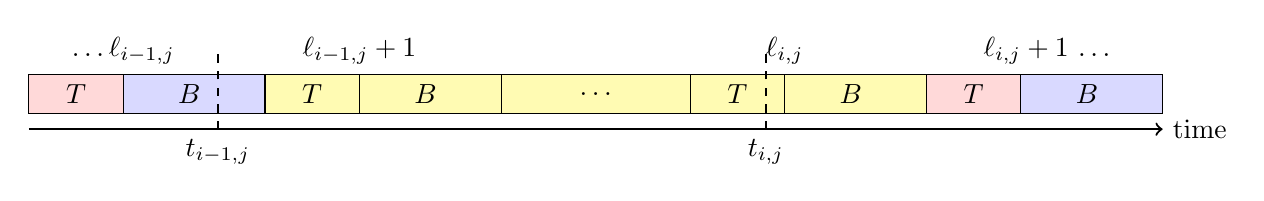
\begin{tikzpicture}[xscale=1.2, yscale=1]

    % Timeline
    \draw[thick, ->] (0,0) -- (12,0) node[right] {time};

    % epoch labels
    \node at (1,1) {\dots \(\ell_{i-1,j}\)};
    \node at (3.5,1) {\(\ell_{i-1,j}+1\)};
    \node at (8,1) {\(\ell_{i,j}\)};
    \node at (10.8,1) {\(\ell_{i,j}+1\) \dots};

    % Highlight interval
    \draw[fill=yellow!30] (2.5,0.2) rectangle (10.5,0.7);
    \node at (6,0.45) {\(\dots\)};

    % Example epochs
    \draw[fill=red!15] (0,0.2) rectangle (1,0.7);
    \node at (0.5,0.45) {\(T\)};
    \draw[fill=blue!15] (1,0.2) rectangle (2.5,0.7);
    \node at (1.7,0.45) {\(B\)};

    \draw[fill=yellow!30] (2.5,0.2) rectangle (3.5,0.7);
    \node at (3,0.45) {\(T\)};
    \draw[fill=yellow!30] (3.5,0.2) rectangle (5,0.7);
    \node at (4.2,0.45) {\(B\)};

    \draw[fill=red!15] (9.5,0.2) rectangle (10.5,0.7);
    \node at (10,0.45) {\(T\)};
    \draw[fill=blue!15] (10.5,0.2) rectangle (12,0.7);
    \node at (11.2,0.45) {\(B\)};

    \draw[fill=yellow!30] (7,0.2) rectangle (8,0.7);
    \node at (7.5,0.45) {\(T\)};
    \draw[fill=yellow!30] (8,0.2) rectangle (9.5,0.7);
    \node at (8.7,0.45) {\(B\)};

    % Mark t_{i-1,j} and t_{i,j}
    \draw[dashed, thick] (2,0) -- (2,1);
    \node[below] at (2,0) {\(t_{i-1,j}\)};

    \draw[dashed, thick] (7.8,0) -- (7.8,1);
    \node[below] at (7.8,0) {\(t_{i,j}\)};

    \end{tikzpicture}
    \caption{Timeline illustrating the epochs \(\ell_{i-1,j}+1,\dots, \ell_{i,j}\) in yellow. Note that the periods \(t_{i-1,j}\) and \(t_{i,j}\) are ``offset'' from the beginning and end of the epochs they define.}
    \label{fig:main-ell-interval}
\end{figure}

With this control of \(\Delta_{i_t^*,j}\), the remaining task is to determine how many times the suboptimal arm \(j\) is selected during each interval of epochs \([\ell_{n-1,j}+1, \ell_{n,j}]\). By the definition of \(t_{i,j}\) in \eqref{eq:main-tij}, we know, up to integer ambiguity, the number of plays of arm \(j\) at these stopping times. However, because of the delay between the initiation of a replacement and its completion, together with the blocking rule that forces the solution to remain fixed, the periods \(t_{i-1,j}\) and \(t_{i,j}\) do not align with the boundaries of the epochs \(\ell_{i-1,j}+1,\dots, \ell_{i,j}\), where we control \(\Delta_{i_t^*,j}\). Figure~\ref{fig:main-ell-interval} illustrates this offset: the periods \(t_{i-1,j}\) and \(t_{i,j}\) lie to the left of the epoch boundaries that define the highlighted interval.

For the periods between \(t_{i-1,j}\) and \(d_{\ell_{i-1,j}+1}\)---the first period of epoch \(\ell_{i-1,j}+1\); see \eqref{eq:c-def}---the optimality gap \(\Delta_{i_t^*,j}\) cannot be bounded by \(\Delta_{i-1,j}\) via Lemma~\ref{lem:gap-bound}. However, the \emph{number of plays} of arm \(j\) in the periods \(d_{\ell_{i-1,j}+1},\dots, p_{\ell_{i,j}}\), which lie within the epoch interval \(\ell_{i-1,j}+1,\dots, \ell_{i,j}\), cannot exceed the number of plays in the periods \(t_{i-1,j},\dots, p_{\ell_{i,j}}\), since \(t_{i-1,j}\leq d_{\ell_{i-1,j}+1}\) and the play count is nondecreasing over time. We may therefore decompose the relevant time periods as
\[
    \{t:t_{i-1,j}\leq t < t_{i,j}\} \cup  \{t:t_{i,j}\leq t \leq p_{\ell_{i,j}}\}.
\]
The number of plays in the left set can be bounded by the difference
\[
    \frac{4\log T}{\Delta_{i,j}^2} - \frac{4\log T}{\Delta_{i-1,j}^2}
\]
using the definition of \(t_{i,j}\). Combining this play-count bound with the bound on \(\Delta_{i_t^*,j}\), and then telescoping over the index \(i\), yields the leading \(\log T/\Delta_{m,j}\) term. The number of plays in the right set can be bounded using the block threshold \(N(\ell)\). Careful accounting, together with a second telescoping sum, produces the secondary \(\sqrt{\gamma\log T}\left[1+\log(\Delta_{1,j}/\Delta_{m,j})\right]\) contribution and a lower-order remainder of order \(\Delta_{1,j}(\gamma+1)\) (Lemma~\ref{lem:B-final}).

To complete the argument, we bound the regret incurred during the transition phases. During these phases, the arbitrary nature of replacement times obscures the identity of the best omitted optimal arm, so we do not attempt a refined bound on \(\Delta_{i_t^*,j}\). Moreover, suboptimal arms may persist in transition phases even after they can no longer appear in a block phase, for example if their replacements are delayed. Instead, we use a worst-case bound. Each epoch contains at most \(\bar{\omega}\) transition periods, and each such period incurs regret at most \(m\Delta_{1,k} \leq m\), since all gaps lie in \([0,1]\). It therefore suffices to bound the number of epochs completed within \(T\) rounds. The epoch-count bound from the replacement-cost analysis yields at most \(\sqrt{kT/\gamma}+k\) epochs. Putting these pieces together gives the statement of Lemma~\ref{lem:transition-regret},
\[
    (\text{Transition regret})
    \le
    \bar{\omega} m\!\left(\sqrt{\frac{kT}{\gamma}}+k\right).
\]
Combining this with the contribution from the block phases completes the sampling-regret bound. Combining the result further with the replacement-cost bound completes the proof.


\section{Bounding the Switching Regret}
We now turn to bounding the regret due to arm switches. Recall that the length of each epoch is determined by the least played arm in the current target solution. The central challenge is to understand how quickly this minimum play count can grow. Although the process is stochastic, it has a crucial monotonicity property: once an arm has been played a certain number of times, its count can never decrease. This means the minimum can never fall below its past values, and hence it cannot remain close to a fixed level for too many epochs.  

\subsection{Controlling the growth of the minimum play count}
The idea is as follows. Each epoch length is tied to the current minimum, so controlling its growth directly limits how many epochs can occur over a horizon, and therefore how many switches can occur. Because only \(k\) different arms can serve as the minimizer, once all of them have been ``cycled through," the minimum must increase. This implies a packing type bound: the number of epochs with blocks governed by minima near one another is finite and controlled. The next lemma makes this statement precise.  


\begin{lemma}[Local packing in \(X\)-space]\label{lem:local-packing}
    For each epoch \(\ell\), define
    \[
        X(\ell) = \min_{i \in A_{d_\ell}} T_i(d_\ell),
    \]
    the minimum number of plays among the \(m\) arms selected at time \(d_\ell\). Let
    \[
        g(x) := 2\sqrt{\gamma  x} + \gamma 
        \quad \text{ and } \quad 
        N(\ell) := \bigl\lceil g(X(\ell)) \bigr\rceil.
    \]
    Then for any \(a \ge 0\), the number of epochs whose minimum lies in the
    interval \([a,  a + g(a))\) is at most \(k\):
    \[
        \bigl|\{\ell : a  \leq X(\ell) < a + g(a)\}\bigr|  \leq k.
    \]
\end{lemma}

\noindent {\bf Proof.}
    Fix \(a\ge 0\) and consider the set of epochs
    \[
        \mathcal{L}(a) := \{\ell : a  \leq X(\ell) < a + g(a)\}.
    \]
    If \(\mathcal{L}(a)=\emptyset\), there is nothing to prove. Otherwise, list its
    elements in increasing order:
    \[
        \ell_1 < \ell_2 < \cdots < \ell_q,
        \qquad q := |\mathcal{L}(a)|.
    \]
    For each \(\ell_n \in \mathcal{L}(a)\), select an arm \(i_n \in U_{\ell_n}\) that
    attains the minimum, i.e.
    \[
        T_{i_n}(d_{\ell_n}) = X(\ell_n).
    \]
    Because \(X(\ell_n)\in[a,a+g(a))\), we have in particular \(X(\ell_n)\ge a\).
    Since \(g\) is increasing and \(N(\ell_n)=\lceil g(X(\ell_n))\rceil\), it follows that
    \[
        N(\ell_n) \ge g(X(\ell_n)) \ge g(a).
    \]
    Thus by the end of epoch \(\ell_n\),
    \[
        T_{i_n}(d_{\ell_n + 1})
        = T_{i_n}(d_{\ell_n}) + N(\ell_n)
        \ge
        a + g(a).
    \]
    Play counts are nondecreasing over time, so for any later epoch
    \(\ell > \ell_n\), 
    \[
        T_{i_n}(d_\ell) \ge T_{i_n}(d_{\ell_n+1}) \ge a + g(a).
    \]
    In particular, for any \(\ell > \ell_n\) with \(X(\ell)\in[a,a+g(a))\), arm \(i_n\)
    cannot be the minimum again, because its count at the start of epoch \(\ell\)
    already lies at or above \(a+g(a)\), outside the interval.
    
    We now show that the arms \(i_1,\dots,i_q\) are all distinct. Suppose for
    contradiction that \(i_{n'} = i_n\) for some \(1  \leq n' < n  \leq q\).  Then at the start
    of epoch \(\ell_n\) we would have
    \[
        T_{i_n}(d_{\ell_n}) \ge a + g(a),
    \]
    by the argument above applied to the earlier epoch \(\ell_{n'}\). But since \(\ell_n\in\mathcal{L}(a)\), we also have
    \[
        T_{i_n}(d_{\ell_n}) = X(\ell_n) < a + g(a),
    \]
    a contradiction. Hence all \(i_1,\dots,i_q\) are distinct arms. There are only \(k\) arms in total, so \(q  \leq k\). Since
    \(q = |\mathcal{L}(a)|\), we obtain
    \[
        \bigl|\{\ell : a  \leq X(\ell) < a + g(a)\}\bigr|  \leq k,
    \]
    as claimed.
\Halmos  

\subsection{Quadratic growth of the epoch timeline}
We now turn to lifting this bound to a sequence of iterations. Let \(\{\ell_{r}\}_{r\geq 1}\) be a sequence of epochs ordered chronologically (i.e., \(\ell_{1}< \ell_{2}<\cdots < \ell_{r}\)). Note that this sequence need not contain all epochs between \(\ell_1\) and \(\ell_r\). As an illustrative example, we will later consider the sequence of epochs \(\{\ell_r :\exists i>m \text{ with } i\in U_{\ell_r}\}\). The quantity of interest is the minimum number of periods, over all possible trajectories, that could be contained in these epochs. Let us denote this
\[K(r)=\sum_{s=1}^r(|\mathcal{T}_{\ell_s}|+|\mathcal{B}_{\ell_s}|)\]
To fix ideas, note that if \(\{\ell_{r}\}_{r\geq 0}\) is the sequence \(1,2,\dots, r\) (the first \(r\) consecutive epochs), then \(K(r)=d_{r+1}\), the timestamp of the first period of the (\(r+1\))th epoch. Our goal is to show that \(K(r)\) cannot grow too slowly. The key observation is that in each group of \(k\) epochs, the minimum play count must increase according to \(g(x)\). Consequently, the sequence of minima cannot stagnate, because it is bounded below by a deterministic recurrence. 

\begin{lemma}\label{lem:ell-t-bound}
    Let \(\{\ell_{r}\}_{r\geq 1}\) be a sequence of epochs and \(X(\ell_1)\) be the minimum count at the beginning of epoch \(\ell_1\). Then for every  \(r > k\)
    \[
        K(r)
        \ge
        k\left(\sqrt{\gamma}\left(\frac{r}{k} - 1\right)+\sqrt{X(\ell_1)}\right)^2-kX(\ell_1).
    \]
    and for every \(r \leq k\), \(K(r) \geq r\left(2\sqrt{X(\ell_1)}+ \gamma\right)\).
\end{lemma}

\noindent {\bf Proof.}
    From the definition of \TimeToReplace\,\,(Algorithm \ref{alg:TimeToReplace}) we have that the length of an epoch is either the block threshold \(N(\ell)\) or the longest delay, whichever comes last. Thus,
    \[ K(r)=\sum_{s=1}^r|\mathcal{T}_{\ell_s}|+|\mathcal{B}_{\ell_s}|=\sum_{s=1}^r\max\left(N(\ell_r), \max_{(i,j)\in R_{d_{\ell_r}}}\omega_{i,j}^{(d_{\ell_r})}\right)\geq \sum_{s=1}^r N(\ell_r)
    \]
    
    We first consider the case that \(r \leq k\). Then, because 
    \[N(\ell_r)\geq r\cdot  \min_{i\in U_{\ell_r}}\left( 2\sqrt{\gamma T_{i}(t)}+ \gamma\right)\geq r\left(2\sqrt{\gamma X(\ell_1)}+ \gamma\right)\]
    we have the trivial bound \(K(r) \geq r\left(2\sqrt{X(\ell_1)}+ \gamma\right)\). We now prove the case for \(r > k\). As in Lemma~\ref{lem:local-packing}, define \(g(x) := 2\sqrt{\gamma x} + \gamma\) to be the function that maps the minimum play count to a lower bound on the number of plays in the epoch. A natural way to organize the possible values of the minima is to introduce a deterministic sequence
    \[
        a_0 := X(\ell_1), \quad a_{n+1} := a_n + g(a_n).
    \]
    By construction \(a_n = (\sqrt{X(\ell_1)}+n\sqrt{\gamma})^2\) (Lemma \ref{lem:exact-quadratic}) for all \(n\ge 0\).  The sequence \(\{a_n\}\) induces a natural partition of the nonnegative numbers in the \(X\)-space (the space of minimum counts) into the intervals
    \[
        I_n := [ a_n, a_n + g(a_n) ).
    \]
    that can be viewed as ``levels". Because \(g\) is increasing, an epoch whose minimum lies in \(I_n\) must have epoch length at least \(g(a_n)\). Lemma~\ref{lem:local-packing} says that at most \(k\) epochs can have their minima in any particular level \(I_n\). Let \(q_n\) denote the number of the first \(r\) epochs whose minima fall in \(I_n\).
    The packing property ensures that
    \[
        0  \leq q_n  \leq k
        \qquad\text{and}\qquad
        \sum_{n\ge 0} q_n = r.
    \]
    Since each such epoch contributes at least \(g(a_n)\) periods, the total time after
    \(\ell\) epochs satisfies
    \[
        K(r)
        \ge
        \sum_{n\ge 0} q_n  g(a_n).
    \]
    To obtain the smallest possible value of the right-hand side subject to the above constraints, one must fill low levels before higher ones, because \(g(a_n)\) is increasing in \(n\). Thus the minimizing pattern is
    \[
        q_0 = q_1 = \cdots = q_{R-1} = k,
        \qquad R := \left\lfloor {r}/{k}\right\rfloor,
    \]
    with any remaining epochs (if any) placed at level \(L\) or above.  This yields the
    lower bound
    \[
        K(r)
        \ge
        k \sum_{n=0}^{R-1} g(a_n).
    \]
    Because \(a_n = (\sqrt{a_0}+n\sqrt{\gamma})^2\), the increment satisfies \(g(a_{n-1}) = 2\gamma  (n-1) + \gamma\). Thus
    \begin{align*}
        \sum_{n=0}^{R-1} g(a_n)
        &= \sum_{n=1}^{R} g(a_{n-1})
        = \sum_{n=1}^{R} \left(2\sqrt{\gamma (\sqrt{a_0}+(n-1)\sqrt{\gamma})^2} + \gamma\right)\\
        &= \sum_{n=1}^{R} 2\sqrt{\gamma a_0}+\gamma  \sum_{n=1}^{R}2(n-1)  + 1
        = 2R\sqrt{\gamma a_0}+\gamma  R^2 = (\sqrt{\gamma}R+\sqrt{a_0})^2-a_0.
    \end{align*}
    Substituting this into the previous display gives \(K(r)\ge k [(\sqrt{\gamma}R+\sqrt{a_0})^2-a_0]\). Finally, since \(R = \lfloor r/k\rfloor \ge r/k - 1\) and \(r/k - 1\geq 0\) when \(r \geq k\), we have \(R^2 \ge (r/k - 1)^2\),
    and therefore
    \[
        K(r)
        \ge
        k\left(\sqrt{\gamma}\left(\frac{r}{k} - 1\right)+\sqrt{X(\ell_1)}\right)^2-kX(\ell_1)
    \]

    for the second result.
\Halmos

We will frequently invoke the following corollary which follows immediately from  a special case of Lemma~\ref{lem:ell-t-bound}. 
\begin{corollary}[Inverse of \(K(r)\) with \(X(\ell_1)=0\)]\label{cor:inv_K}
    For a given sequence \(\{\ell_r\}_{r\geq 1}\) with \(X(\ell_1)=0\) that contains at most \(y\) periods, we can compute the maximum number of epochs in the sequence by inverting \(K\),
    \[\max\{r: K(r)\leq y\}\leq K^{-1}(y)=\sqrt{\frac{ky}{\gamma }}+k\]
\end{corollary}
%  

\subsection{Final bound on replacement-cost regret}
Finally, we prove a bound on the replacement-cost regret.
\begin{lemma}[Max epochs]\label{lem:max_epochs}
    The maximum number of epochs satisfies
    \[
        L \leq \sqrt{\frac{kT}{\gamma}}+k.
    \]
\end{lemma}
\noindent {\bf Proof.}
    If \(L\leq k\), then we are done. Otherwise, let \(\{\ell_r\}_{r\geq 1}\) be the sequence of epochs \(\ell=1,\dots,r\). This sequence must satisfy
    \[L \leq \max\left\{\ell\geq k: K(r)\leq T\right\}\]
    Since \(X(\ell_1)=0\), Corollary~\ref{cor:inv_K} gives that
    \[L\leq \max\left\{k, K^{-1}(T)\right\}\leq \max\left\{k, \sqrt{\frac{kT}{\gamma }}+k\right\}= \sqrt{\frac{kT}{\gamma}}+k\]
\Halmos  

\begin{lemma}[Gap-free replacement-cost regret]\label{lem:sc-bound-final}
    The replacement-cost regret satisfies
    \[
        J_T \leq cm\sqrt{\frac{kT}{\gamma}}+cmk.
    \]
\end{lemma}
\noindent {\bf Proof.}
    By construction, the number of replacement epochs by time \(T\) is at most \(cm\) times the number of epochs that can be completed within \(T\) rounds. By Lemma \ref{lem:max_epochs},
    \[J_T \leq cm\cdot \left(\sqrt{\frac{kT}{\gamma }}+k\right)=cm\sqrt{\frac{kT}{\gamma}}+cmk\]
\Halmos  

We can also derive an instance-dependent replacement-cost bound using Lemma~\ref{lem:ell-t-bound} together with Corollary \ref{cor:final-phase} (proved in the next section).
\begin{lemma}[Instance-dependent max epochs]\label{lem:delta-max-epoch}
    Define the minimum optimality gap \(\Delta:=\min_{i\leq m, j>m}\Delta_{i,j}\). If \(\Delta>0\), then the maximum number of epochs is bounded by
    \[\bE{L}\leq 2k\left(\left(\sum_{j>m}\frac{2}{\Delta_{m,j}}\right)\sqrt{\frac{\log T}{k\gamma}}+1+\frac{1}{k}+\frac{k}{\gamma T}+\frac{k^2}{T^2}\right)\]
    so that when \(T> k\),
    \[\bE{L}\in O\left(\sum_{j>m}\frac{2}{\Delta_{m,j}}\sqrt{\frac{k\log T}{\gamma}}\right)\]
\end{lemma}
\noindent {\bf Proof.}
    Consider the sequence of epochs that contain at least one suboptimal arm, \(\{\ell_r: U_{\ell_r}\neq A^*\}\). Then \(X(\ell_1)=0\) by definition. Define the event 
    \[\mathcal{G}=\bigcap_{\ell=1}^L\left\{\LCB_i(d_{\ell})\leq \mu_i\leq\UCB_i(d_{\ell}) \text{ for all } i\in[k]\right\}\]
    Additionally, we define 
    \[
    \mathcal{G}_j(t)=\bigg\{\LCB_i(t)<\mu_i<\UCB_i(t) \text{ for all } i\leq m\bigg\} \bigcap ~\bigg\{\LCB_j(t)<\mu_j<\UCB_j(t)\bigg\}
    \]
    Clearly we have that \(\mathcal{G}\) implies \(\mathcal{G}_j(d_{\ell})\) for all \(j\) and \(d_{\ell}\). Therefore, Corollary \ref{cor:final-phase} (see Appendix \ref{sec:sampling_proof}) implies the number of periods in the epochs where at least one suboptimal arm is chosen to be in the target set is at most
    \[\sum_{j>m}\frac{4\log T}{\Delta_{m,j}^2},\]
    after which \(U_{\ell}=[m]\). Thus, the number of epochs \(r\) that contain at least one suboptimal arm must satisfy 
    \[K(r)\leq \sum_{j>m}\frac{4\log T}{\Delta_{m,j}^2}\]
    and therefore the maximum epochs under \(\mathcal{G}\) is bounded
    \[\bE{\left(\sum_{\ell:U_{\ell}\neq A^*}|\mathcal{T}_{\ell}|+|\mathcal{B}_{\ell}|\right)\cdot \ind{\mathcal{G}}}\leq \max\left\{r: K(r)\leq \sum_{j>m}\frac{4\log T}{\Delta_{m,j}^2}\right\}\]
    Applying Corollary~\ref{cor:inv_K},
    \begin{align*}
        r&\leq K^{-1}\left(\sum_{j>m}\frac{4\log T}{\Delta_{m,j}^2}\right)=\sqrt{\frac{k}{\gamma}\sum_{j>m}\frac{4\log T}{\Delta_{m,j}^2}}+k\\
        &\leq \left(\sum_{j>m}\frac{2}{\Delta_{m,j}}\right)\sqrt{\frac{k\log T}{\gamma}}+k
    \end{align*}
    The last inequality follows from \(\|1/x\|_2\leq \|1/x\|_1\) for all positive \(x\). We conclude that 
    \[\bE{\left(\sum_{\ell:U_{\ell}\neq A^*}|\mathcal{T}_{\ell}|+|\mathcal{B}_{\ell}|\right)\cdot \ind{\mathcal{G}}}\leq \left(\sum_{j>m}\frac{2}{\Delta_{m,j}}\right)\sqrt{\frac{k\log T}{\gamma}}+k\]
    Next we consider the sequence of epochs where \(U_{\ell}=A^*\) under \(\mathcal{G}\), that is, epochs with no suboptimal arm. Recall that the epoch counter increases only when the solution \(U_{\ell}\) changes. Since every epoch in this sequence has the same solution, \(U_{\ell}= A^*\), it must be true that the epoch preceding each epoch in the sequence has \(U_{\ell}\neq A^*\) (except perhaps the initial set \(U_0\)). Thus there is an injective mapping between epochs with \(U_{\ell}=A^*\) and epochs with \(U_{\ell}\neq A^*\). Therefore, under \(\mathcal{G}\), we can also bound the number of epochs with \(U_{\ell}=A^*\) by the number of epochs with \(U_{\ell}\neq A^*\),
    \[\bE{\left(\sum_{\ell:U_{\ell}= A^*}|\mathcal{T}_{\ell}|+|\mathcal{B}_{\ell}|\right)\cdot \ind{\mathcal{G}}}\leq \left(\sum_{j>m}\frac{2}{\Delta_{m,j}}\right)\sqrt{\frac{k\log T}{\gamma}}+k\]
    Thus we have that 
    \[\bE{L\cdot \ind{\mathcal{G}}}\leq \bE{L\mid \mathcal{G}}\leq \left(\sum_{j>m}\frac{4}{\Delta_{m,j}}\right)\sqrt{\frac{k\log T}{\gamma}}+2k+2\]
    Now we count the epoch under the complement event. From Hoeffding's inequality and a union bound,
    \[\bP{\mathcal{G}^c}\leq \bE{\sum_{\ell=1}^L \frac{2k}{T^2}}=\bE{\frac{2Lk}{T^2}}\leq \left(\sqrt{\frac{kT}{\gamma}}+k\right)\frac{2k}{T^2}\]
    The last inequality is Lemma \ref{lem:max_epochs}, which states the most epochs that can occur in \(T\) periods is deterministically less than \(\sqrt{kT /\gamma}+k\).
    Again using Lemma \ref{lem:max_epochs} to bound \(\bE{L\mid \mathcal{G}^c}\),
    \[\bE{L\cdot \ind{\mathcal{G}^c}}=\bP{\mathcal{G}^c}\bE{L\mid \mathcal{G}^c}\leq \left(\sqrt{\frac{kT}{\gamma}}+k\right)^2\frac{2k}{T^2}\leq 2k\left(\frac{k}{\gamma T}+\frac{k^2}{T^2}\right)\]
    Thus,
    \[\bE{L}\leq 2k\left(\left(\sum_{j>m}\frac{2}{\Delta_{m,j}}\right)\sqrt{\frac{\log T}{k\gamma}}+1+\frac{1}{k}+\frac{k}{\gamma T}+\frac{k^2}{T^2}\right)\]
    so that when \(T> k\),
    \[\bE{L}\in O\left(\left(\sum_{j>m}\frac{1}{\Delta_{m,j}}\right)\sqrt{\frac{k\log T}{\gamma}}\right)\]
\Halmos

Similarly, we can derive an instance-dependent replacement-cost regret.
\begin{lemma}[Instance-dependent replacement-cost regret]\label{lem:delta-sc-bound-final}
    Denote the minimum optimality gap \(\Delta:=\min_{i\leq m, j>m}\Delta_{i,j}\). If \(\Delta>0\),
    \begin{align*}
        J_T&\leq 2cmk\left(\left(\sum_{j>m}\frac{2}{\Delta_{m,j}}\right)\sqrt{\frac{\log T}{k\gamma}}+1+\frac{1}{k}+\frac{k}{\gamma T}+\frac{k^2}{T^2}\right)
    \end{align*}
    and when \(T>k\),
    \[J_T\in O\left(\left(\sum_{j>m}\frac{1}{\Delta_{m,j}}\right)\cdot cm\sqrt{\frac{k\log T}{\gamma}}\right)\]
\end{lemma}
\noindent {\bf Proof.}
    By construction, the number of replacement epochs by time \(T\) is at most \(cm\) times the number of epochs that can be completed within \(T\) rounds. By Lemma \ref{lem:delta-max-epoch},
    \[J_T\leq \bE{cmL}\leq cmk\left(\left(\sum_{j>m}\frac{1}{\Delta_{m,j}}\right)\sqrt{\frac{\log T}{k\gamma}}+1+\frac{1}{k}+\frac{2k}{\gamma T}+\frac{2k^2}{T^2}\right)\]
This completes the proof. 
\Halmos  


\section{Bounding the Sampling Regret}\label{sec:sampling_proof}
Recall that for a fixed suboptimal arm \(j\), the regret contribution is determined by the best available optimal arm that was not chosen,
$i^*_t = \argmax_{i \in A^* \setminus A_t} \mu_i$.
A naive upper bound of the form \(\Delta_{i^*_t,j} \leq \Delta_{1,j}\) is too coarse to yield tight guarantees, since it ignores the fact that the identity of \(i^*_t\) depends on all of \(A_t\), and not just \(j\). The challenge is that, unlike in the single-arm setting, eliminating \(j\) requires comparing it not just to the best arm overall, but successively to each optimal arm. In other words, regret may persist against weaker optimal arms even after \(j\) has been statistically separated from the strongest one.

This difficulty is compounded by two sources of randomness: (i) the block threshold \eqref{eq:block-threshold} is defined by a \emph{minimum} over play counts, which makes both the start time and the length of each epoch random and history dependent; and (ii) delayed action means that the set of comparisons relevant at time \(t\) is itself subject to the delay process. These features prevent a straightforward elimination argument.

To overcome this, we introduce a sequence of random intervals that align with the successive times at which arm \(j\) can be distinguished from each optimal arm \(i\). Within each interval, the regret from pulling \(j\) can be tightly bounded by the gap \(\Delta_{i,j}\), reflecting that \(j\) can only be confused with optimal arms weaker than \(i\). The problem is thus reduced to showing that the total length of these intervals is well controlled. By carefully bounding their expected duration, we obtain the sharper regret bound stated in Lemma \ref{lem:B-final}.


\subsection{Constructing Elimination Intervals}
The analysis of regret depends on how we compare the chosen suboptimal arm \(j>m\) against the best available alternative, $i_t^*$. To organize the analysis, we introduce what we call \emph{distinguishability intervals}, a sequence of random stopping intervals that partition the horizon according to when each suboptimal arm becomes statistically distinguishable from the optimal set. This construction generalizes standard arm elimination arguments used in classical UCB analysis to the delayed and multi-play setting. The intervals serve as a proof device that filters the history to isolate the moments where meaningful comparisons can be made between the chosen arm and the best available alternative. Within each interval, the gap \(\Delta_{i^*_t,j}\) can be bounded more sharply than by the trivial inequality, and the overall regret can then be controlled by bounding the lengths of these intervals.

Formally, define the stopping time
\[
t_{i,j} = \min\left\{t\in \mathbb{N} : T_j(t) > \frac{4\log T}{\Delta^2_{i,j}}\right\},
\]
with the convention \(t_{i,j}=\infty\) if the set is empty. Intuitively, \(t_{i,j}\) is the first time (under the good event) when the learner has accumulated enough samples of arm \(j\) to statistically separate it from arm \(i\); that is, the point at which arm \(j\) becomes distinguishable from arm \(i\). 

We then define the epoch index $\ell_{i,j} = \epoch(t_{i,j})$,
corresponding to the epoch that contains \(t_{i,j}\). Because the algorithm updates the UCBs once per epoch, the information that \(t_{i,j}\) has occurred will not be incorporated until epoch \(\ell_{i,j} + 1\). The resulting sequence of stopping intervals
\(\{[\ell_{i-1,j}+1, \ell_{i,j}+1)\}\)
forms the distinguishability intervals that structure the analysis throughout the subsequent regret decomposition. See Figure \ref{fig:elimination-timeline} for the timeline.

\begin{figure}[t]
    \centering
    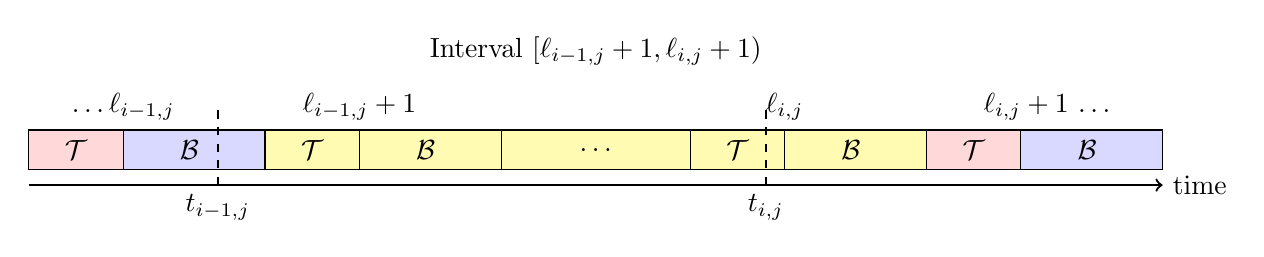
\begin{tikzpicture}[xscale=1.2, yscale=1]
    
    % Timeline
    \draw[thick, ->] (0,0) -- (12,0) node[right] {time};
    
    % epoch labels
    \node at (1,1) {\dots \(\ell_{i-1,j}\)};
    \node at (3.5,1) {\(\ell_{i-1,j}+1\)};
    \node at (6,1.7) {Interval \([\ell_{i-1,j}+1, \ell_{i,j}+1)\)};
    \node at (8,1) {\(\ell_{i,j}\)};
    \node at (10.8,1) {\(\ell_{i,j}+1\) \dots};
    
    % Highlight interval
    \draw[fill=yellow!30] (2.5,0.2) rectangle (10.5,0.7);
    \node at (6,0.45) {\(\dots\)};
    
    % Example epochs
    \draw[fill=red!15] (0,0.2) rectangle (1,0.7);
    \node at (0.5,0.45) {\(\mathcal{T}\)};
    \draw[fill=blue!15] (1,0.2) rectangle (2.5,0.7);
    \node at (1.7,0.45) {\(\mathcal{B}\)};

    \draw[fill=yellow!30] (2.5,0.2) rectangle (3.5,0.7);
    \node at (3,0.45) {\(\mathcal{T}\)};
    \draw[fill=yellow!30] (3.5,0.2) rectangle (5,0.7);
    \node at (4.2,0.45) {\(\mathcal{B}\)};

    \draw[fill=red!15] (9.5,0.2) rectangle (10.5,0.7);
    \node at (10,0.45) {\(\mathcal{T}\)};
    \draw[fill=blue!15] (10.5,0.2) rectangle (12,0.7);
    \node at (11.2,0.45) {\(\mathcal{B}\)};

    \draw[fill=yellow!30] (7,0.2) rectangle (8,0.7);
    \node at (7.5,0.45) {\(\mathcal{T}\)};
    \draw[fill=yellow!30] (8,0.2) rectangle (9.5,0.7);
    \node at (8.7,0.45) {\(\mathcal{B}\)};
    
    % Mark t_{i-1,j} and t_{i,j}
    \draw[dashed, thick] (2,0) -- (2,1);
    \node[below] at (2,0) {\(t_{i-1,j}\)};
    
    \draw[dashed, thick] (7.8,0) -- (7.8,1);
    \node[below] at (7.8,0) {\(t_{i,j}\)};
    
    \end{tikzpicture}
    \caption{Timeline illustrating a single distinguishability interval for arm \(j\). The interval \([\ell_{i-1,j}+1, \ell_{i,j}+1)\) is shaded yellow, and the corresponding periods \(t_{i-1,j}\) and \(t_{i,j}\) are marked.}
    \label{fig:elimination-timeline}
\end{figure}

Our first lemma establishes that once sufficient evidence has accumulated to distinguish a suboptimal arm \(j\) from some optimal arm \(i\), the algorithm will never prefer \(j\) over \(i\). This parallels the classical UCB elimination lemma, but with an important caveat: because of the availability constraints and the constrained selection rule, we cannot immediately conclude that whenever \(j\) is played, arm \(i\) must also be played.

Define a ``good event''
\[
    \mathcal{G}_j(t)=\bigg\{\LCB_i(t)<\mu_i<\UCB_i(t) \text{ for all } i\leq m\bigg\} \bigcap ~\bigg\{\LCB_j(t)<\mu_j<\UCB_j(t)\bigg\}
\]
to be the event that \(j\) is well estimated and all optimal arms \(i\leq m\) (\(i\in A^*\)) are well estimated. The next step is to understand how the stopping times \(\ell_{i,j}\) are ordered as \(i\) ranges over the optimal arms. The following lemma shows that these times occur in a natural sequence, beginning at the start of the process and ending with the final elimination of \(j\).

\begin{lemma}\label{lem:ordered-intervals}
    For any suboptimal arm \(j>m\), recalling the convention \(\ell_{0,j}:=1\), we have
    \[\ell_{0,j}\leq \ell_{1,j}\leq \ell_{2,j}\leq \cdots \leq \ell_{m,j}\]
\end{lemma}
\noindent {\bf Proof.}
    Observe that \(\Delta_{1,j}>\Delta_{2,j}>\cdots >\Delta_{m,j}\) implies 
    \[\frac{4\log T}{\Delta^2_{1,j}}<\frac{4\log T}{\Delta^2_{2,j}}<\cdots < \frac{4\log T}{\Delta^2_{m,j}}\]
    Recall that 
    \[t_{i,j} = \min\left\{t\in \mathbb{N}:T_j(t)>\frac{4\log T}{\Delta^2_{i,j}}\right\}\]
    where \(T_j(t)\) is the count of times arm \(j\) has been played by time \(t\). Then we must have that 
    \[T_j(t_{1,j})\leq T_j(t_{2,j})\leq \cdot \leq T_j(t_{m,j})\]
    with equality arising from the restriction \(t\in \mathbb{N}\). Additionally, \(T_j(\cdot)\) is a count, so it is monotonically nondecreasing in its argument. This implies that 
    \[t_{1,j}\leq t_{2,j} \leq \cdots \leq t_{m,j}\]
    By the monotonicity of the \(\epoch(\cdot)\) function we have 
    \[\ell_{1,j}\leq \ell_{2,j}\leq \cdots \leq \ell_{m,j}\]
The proof is complete.
\Halmos  

This ordering allows us to define the distinguishability intervals. Each interval \([\ell_{i-1,j}+1, \ell_{i,j}+1)\) corresponds to a phase of the algorithm where arm \(j\) is distinguishable from the best \(i-1\) optimal arms. Once \(j\) can be separated from all \(m\) optimal arms, it is eliminated permanently. Formally, the \emph{distinguishability intervals} form a random partition of the following form:
\[
[1,L]=\left(\bigcup_{i=1}^m [\ell_{i-1,j}+1, \ell_{i,j}+1)\right)\cup \{\ell\geq \ell_{m,j}+1\}.
\]
Note that an interval may be empty if two stopping times \(\ell_{i,j}\) and \(\ell_{i+1,j}\) occur in the same epoch. The intervals thus filter the history into exactly the stages where the regret incurred by playing \(j\) can be successively bounded. This gives the needed structure to address the availability constraints. However, we still must address the constraint in the selection rule.

We want to show that if an optimal arm \(i\) has higher upper confidence bound than \(j\) and arm \(i\) is available, then \(j\) will not be played. However, recall that the optimization problem \eqref{eq:opt} has a constraint 
\[\sum_{j\in A_t\setminus U}\delta_{j,i}(t)\geq |A_t\setminus U|\cdot \frac{c}{T-t}\]


\begin{lemma}
\label{lem:monotonicity-selection}
    Let \(i,j\) be arms such that
    \[
    \UCB_i(t)>\UCB_j(t)
    \qquad\text{and}\qquad
    \delta_{j,i}(t):=\UCB_i(t)-\LCB_j(t)\ge \frac{c}{T-t}.
    \]
    Let \(U\) be an optimal solution to \eqref{eq:opt}. Then
    \[
    j\in U \implies  i\in U.
    \]
\end{lemma}

\noindent\textbf{Proof.}
    We argue by contradiction. Suppose \(j\in U\) but \(i\notin U\). We show that in either case one can construct a feasible target set with strictly larger objective value, contradicting the optimality of \(U\). We consider the target set \(U' := \bigl(U\setminus\{j\}\bigr)\cup\{i\}\). Because \(\UCB_i(t)>\UCB_j(t)\) the objective value of \(U'\) is strictly larger than that of \(U\). Therefore, if \(U'\) is feasible we have derived a contradiction. We prove feasibility in two cases.
    
    \textit{Case 1: \(j\notin A_t\).}
    Then \(j\in U\setminus A_t\), so \(j\) is entering the target set and \(|A_t\setminus U|=|A_t\setminus U'|\). Consider the target set \( U' := \bigl(U\setminus\{j\}\bigr)\cup\{i\}. \)
    Since \(j\in U\setminus A_t\), feasibility of \(U\) implies
    \begin{align*}
        \sum_{s\in A_t\setminus U'} \delta_{s,\pi^{\mathrm R}(s)}(t)&=\sum_{s\in A_t\setminus U'}\bigg[\UCB_{\pi^{\mathrm R}(s)}(t)-\LCB_s(t)\bigg]\\
        &=\sum_{s\in A_t\setminus U}\bigg[\UCB_{\pi^{\mathrm R}(s)}(t)-\LCB_s(t)\bigg]+ \bigg(\UCB_i(t)-\UCB_j(t)\bigg)\\
        &\ge \bigg(\UCB_i(t)-\UCB_j(t)\bigg)+|A_t\setminus U|\frac{c}{T-t}\\
        &=\bigg(\UCB_i(t)-\UCB_j(t)\bigg)+|A_t\setminus U'|\frac{c}{T-t}.\\
    \end{align*}
    Because \(\UCB_i(t)>\UCB_j(t)\), we conclude that 
    \[\sum_{s\in A_t\setminus U'} \delta_{s,\pi^{\mathrm R}(s)}(t)\ge |A_t\setminus U'|\frac{c}{T-t}\]
    so \(U'\) is feasible. 
    
    \textit{Case 2: \(j\in A_t\).}
    In this case, \(j\in U\cap A_t\), so \(j\) is retained in the workforce and \(|A_t\setminus U|+1=|A_t\setminus U'|\). Therefore,
    \begin{align*}
        \sum_{s\in A_t\setminus U'} \delta_{s,\pi^{\mathrm R}(s)}(t)&=\sum_{s\in A_t\setminus U'}\bigg[\UCB_{\pi^{\mathrm R}(s)}(t)-\LCB_s(t)\bigg]\\
        &=\sum_{s\in A_t\setminus U}\bigg[\UCB_{\pi^{\mathrm R}(s)}(t)-\LCB_s(t)\bigg]+ \bigg(\UCB_i(t)-\LCB_j(t)\bigg)\\
        &\ge \bigg(\UCB_i(t)-\LCB_j(t)\bigg)+\sum_{s\in A_t\setminus U}\frac{c}{T-t}\\
        &\ge \frac{c}{T-t}+\sum_{s\in A_t\setminus U}\frac{c}{T-t}=(|A_t\setminus U|+1)\frac{c}{T-t}=|A_t\setminus U'|\frac{c}{T-t}.\\
    \end{align*}
    This proves that \(U'\) is feasible when \(j\in A_t\) as well.
    
    In both cases, the assumption \(j\in U\) and \(i\notin U\) leads to a contradiction. Therefore \(j\in U\) implies \(i\in U\).\Halmos 

With this result in hand, we can prove the elimination lemma.
\begin{lemma} \label{lem:gap-bound}
    For any suboptimal arm \(j>m\) and optimal arm \(i\leq m\), if \(\ell> \ell_{i,j}\) and \(t\in \mathcal{B}_{\ell}\), then under the good event \(\mathcal{G}_j(d_\ell)\) and the horizon event \(\{\Delta_{i^*_t, j}> c/(T-t)\}\), we have 
 \(\Delta_{i^*_t,j}\leq \Delta_{i,j}\). 
\end{lemma}
\noindent {\bf Proof.}
    Suppose for contradiction that \(i^*_t\leq i\). Let \(\ell > \ell_{i,j}\). Then the target solution corresponding to epoch \(\ell\) is computed in time instant \(d_\ell\). Observe that 
    for every \(\ell\), \( d_\ell \leq  p_\ell \leq  d_{\ell+1}\),
    with equality \(p_\ell=d_{\ell +1}\) possible if the least-played arm is played \(N(\ell)\) times before \(U_{\ell}\) becomes available. Therefore,
    \[d_\ell\geq d_{\ell_{i,j}+1} \geq d_{\ell_{i^*_t,j}+1}\geq t_{i^*_t,j}\]
    Since the play count of arm \(j\), \(T_j(\cdot)\), is monotonically nondecreasing in its argument, we must have \(T_j(d_\ell)\geq T_j(t_{i^*_t,j})\). 
    Plugging in the definition of \(t_{i^*_t,j}\) gives
    \[T_j(d_\ell)\geq T_j(t_{i^*_t,j})>\frac{4\log T}{\Delta^2_{i^*_t,j}}\]
    It then follows from Lemma~\ref{lem:arm-comp} that under the event \(\mathcal{G}_j(d_\ell)\), we have \(\UCB_j(d_\ell)<\UCB_{i^*_t}(d_\ell)\).
    This implies that replacing \(j\) with \(i^*_t\) increases the objective. Moreover, under \(\mathcal{G}_j(d_{\ell})\) we have \(\delta_{i^*_t,j}\geq \Delta_{i^*_t,j}\). Then on the event \(\Delta_{i^*_t, j}> c/(T-t)\) we conclude
    \[(T-t)\delta_{i^*_t,j}\geq (T-t)\Delta_{i^*_t,j}\geq c\]
    Since \(\UCB_j(d_\ell)<\UCB_{i^*_t}(d_\ell)\) and \((T-t)\delta_{i^*_t,j}\geq c\), Lemma \ref{lem:monotonicity-selection} yields that \(i^*_t\) must be in the target set, that is, \(i^*_t\in U_{\ell}\). Moreover, because \(t\in \mathcal{B}_\ell\), the arms in \(U_{\ell}\) are active by definition. However, this implies that the algorithm plays arm \(i^*_t\), contradicting the definition of \(i^*_t\) as the best unplayed arm. We conclude that we must have \(i^*_t>i\). It then follows from the ordering of means \(\mu_1 > \mu_2 > \dots > \mu_k\) that
    \[i^*_t>i\implies \Delta_{i^*_t,j}\leq \Delta_{i,j}\]
The result thus follows. 
\Halmos  

A direct corollary of Lemma \ref{lem:gap-bound} is that every suboptimal arm is eventually eliminated from the target solution once it becomes distinguishable from the worst optimal arm.
\begin{corollary} \label{cor:final-phase}
    For any suboptimal arm \(j>m\), if \(\ell> \ell_{m,j}\), then under the good event \(\mathcal{G}_j(d_\ell)\), we have \(j\not\in U_{\ell}\).
\end{corollary}
\noindent {\bf Proof.}
    Suppose for contradiction that \(j\in U_\ell\). This implies that there exists \(i\leq m\) that is not in \(U_{\ell}\). This means that \(i^*_t\leq m\), which contradicts Lemma \ref{lem:gap-bound}.
\Halmos  

\subsection{Bounding the regret from the block phase}
We begin with the contribution to regret arising during the block phases. To do this, we condition on \(\mathcal{G}_j(d_\ell)\) for each \(1\leq \ell \leq L\).
\begin{eqnarray*}
   \bE{\sum_{\ell =1}^L \sum_{t\in \mathcal{B}_\ell}\Delta_{i^*_t, j} \ind{j\in U_{\ell}}}
    &\leq& \bE{\sum_{\ell =1}^L \sum_{t\in \mathcal{B}_\ell}\Delta_{i^*_t, j} \ind{j\in U_{\ell},\mathcal{G}_j(d_\ell)}} \\
    &&+ \bE{\sum_{\ell =1}^L \sum_{t\in \mathcal{B}_\ell}\Delta_{i^*_t, j} \ind{j\in U_{\ell},\mathcal{G}^c_j(d_\ell)}}
\end{eqnarray*}
We begin by bounding the complement event.


\begin{lemma}\label{lem:block-complement-regret}
For any \(j\in[k]\). Let \(\mathcal{B}_\ell\) denote the block phase in epoch \(\ell\). Then, for \(k\ge 2\),
\[
    \bE{\sum_{\ell =1}^L \sum_{t\in \mathcal{B}_\ell}\Delta_{i^*_t, j} \ind{j\in U_{\ell},\mathcal{G}^c_j(d_\ell)}} 
    \le
    \frac{4m\Delta_{1,j}}{T}.
\]
In particular, when \(T>m\) the contribution of \(\mathcal{G}_j^c\) is
\(O\!\left(1\right)\).
\end{lemma}
\noindent {\bf Proof.}
    Note that Lemma \ref{lem:Gc} gives \(\bP{\mathcal{G}_j^c(d_{\ell})}\leq 4m/T^2\) for any \(j\) and any realization of \(d_\ell\). Thus,
    \begin{align*}
        \bE{\sum_{\ell =1}^L \sum_{t\in \mathcal{B}_\ell}\Delta_{i^*_t, j} \ind{j\in U_{\ell},\mathcal{G}^c_j(d_\ell)}} 
        &\leq \bE{\sum_{\ell =1}^L \sum_{t\in \mathcal{B}_\ell}\Delta_{i^*_t, j} \ind{\mathcal{G}^c_j(d_\ell)}} \\
        &\leq \Delta_{1,j}\bE{\sum_{\ell =1}^L \sum_{t\in \mathcal{B}_\ell} \ind{\mathcal{G}^c_j(d_\ell)}} \\
        &\leq  \Delta_{1,j}T\left(\frac{4m}{T^2}\right) \leq \frac{4m\Delta_{1,j}}{T} 
    \end{align*}
\Halmos

% \noindent {\bf Proof.}
% Let \(\{\mathcal{F}_t\}\) be the filtration generated by the algorithm.
% Conditional on \(\mathcal{F}_{d_\ell}\), \(\tau_\ell\) is a stopping time and is bounded by
% the block threshold \(N(\ell)\) by construction. Using the definition of \(N(\ell)\),
% \[\tau_{\ell}\leq N(\ell)=\min_{u\in U_\ell}\left\lceil 2\sqrt{\gamma T_u(d_\ell)}+\gamma \right\rceil \le2\sqrt{\gamma d_\ell}+\gamma
% \]
% since \(T_u(d_\ell) \leq d_\ell\). Therefore,
% \begin{align*}
%     \bE{\sum_{\ell =1}^L \sum_{t\in \mathcal{B}_\ell}\Delta_{i^*_t, j}
%     \ind{j\in U_{\ell},\mathcal{G}^c_j(d_\ell)}} & \leq \sum_{\ell\ge 1}\Delta_{1,j} \bE{\sum_{t\in \mathcal{B}_\ell}\ind{\mathcal{G}^c_j(d_\ell)}}\\
%     &= \sum_{\ell\ge 1}\Delta_{1,j} \bE{\tau_\ell}\cdot \bP{\mathcal{G}^c_j(d_\ell)}.
% \end{align*}
% By Lemma~\ref{lem:const-regret}, we have
% \[
%     \bP{\mathcal{G}^c_j(d_\ell)\mid d_\ell}\le\frac{3}{m(kd_\ell)^2}.
% \]
% Taking expectation and using the bound on \(N(\ell)\) yields
% \begin{eqnarray*}
%   \bE{\tau_\ell}\cdot \bP{\mathcal{G}^c_j(d_\ell)} &=& \bE{\bE{\tau_\ell\mid d_\ell}\cdot \bP{\mathcal{G}^c_j(d_\ell)\mid d_\ell}}\\
%     &\leq& \bE{\left(2\sqrt{\gamma d_\ell}+\gamma\right)\cdot \frac{3}{m(kd_\ell)^2}}\leq \frac{6\sqrt{\gamma}}{m k^2}\bE{d_\ell^{-3/2}} + \frac{3\gamma}{m k^2}\bE{d_\ell^{-2}}.
% \end{eqnarray*}
% We now invoke Lemma~\ref{lem:ell-t-bound}. Since it provides lower bounds on \(d_{\ell+1}\), we apply it with index \(\ell-1\). We consider two cases. First, when \(\ell \leq k+1\) then \(\ell-1 \leq k\), so Lemma~\ref{lem:ell-t-bound} gives $d_\ell = d_{(\ell-1)+1} \ge \gamma(\ell-1).$
% Hence,
% \begin{align*}
%     \bE{\tau_\ell}\cdot \bP{\mathcal{G}^c_j(d_\ell)}& \leq \frac{6\sqrt{\gamma}}{m k^2(\gamma(\ell-1))^{3/2}} +\frac{3\gamma}{m k^2(\gamma(\ell-1))^{2}}\\
%     &=\frac{6}{m\gamma k^2(\ell-1)^{3/2}} + \frac{3}{m\gamma k^2(\ell-1)^{2}}
% \end{align*}
% Summing over \(\ell=2,\dots,k+1\), set \(r=\ell - 1\), and let \(\zeta(r)\) denote the Riemann zeta function.
% \begin{align*}
%     \sum_{\ell=2}^{k+1} \bE{\tau_\ell}\cdot \bP{\mathcal{G}^c_j(d_\ell)}& \leq \frac{1}{m\gamma k^2} \left( 6\sum_{r=1}^k\frac{1}{r^{3/2}}+3\sum_{r=1}^k\frac{1}{r^2}\right)\\
%     & \qquad\qquad \leq \frac{1}{m\gamma k^2} \left( 6\zeta(3/2)+3\zeta(2)\right)
%     < \frac{21}{m\gamma k^2}
% \end{align*}
% Secondly, we consider the case \(\ell-1>k\). Then Lemma~\ref{lem:ell-t-bound} gives
% \[
%     d_\ell = d_{(\ell-1)+1} \ge \gamma k\Big(\frac{\ell-1}{k}-1\Big)^2 = \frac{\gamma}{k}(\ell-k-1)^2.
% \]
% Using this lower bound,
% \[
%     \frac{1}{k^2 d_\ell^{3/2}}  \leq \frac{1}{\gamma^{3/2}\sqrt{k} r^3},
% \]
% and 
% \[
%     \frac{1}{k^2 d_\ell^{2}}  \leq \frac{1}{\gamma^{2} r^4}.
% \]
% Therefore,
% \begin{align*}
%     \sum_{\ell=k+2}^{\infty}
%     \bE{\tau_\ell}\cdot \bP{\mathcal{G}^c_j(d_\ell)} &\le
%     \frac{6\sqrt{\gamma}}{m}\sum_{r=1}^\infty \frac{1}{\gamma^{3/2}\sqrt{k}r^3} +\frac{3\gamma}{m}\sum_{r=1}^\infty \frac{1}{\gamma^{2} r^4}\\
%     &= \frac{6\zeta(3)}{m\gamma\sqrt{k}} + \frac{3\zeta(4)}{m\gamma}
%     <\frac{8}{m\gamma\sqrt{k}} + \frac{4}{m\gamma}
% \end{align*}
% Combining the two cases and multiplying by \(\Delta_{1,j}\) yields
% \[
%     \bE{\sum_{\ell =1}^L \sum_{t\in \mathcal{B}_\ell}\Delta_{i^*_t, j}\ind{j\in U_{\ell},\mathcal{G}^c_j(d_\ell)}} \leq \Delta_{1,j}\left(\frac{8}{m\gamma\sqrt{k}} + \frac{4}{m\gamma}+\frac{21}{m\gamma k^2}\right),
% \]
% which completes the proof.
% \Halmos  

Now we bound the sampling regret under the good event. By construction of the distinguishability intervals, we can decompose the total block phase regret as
\begin{align*}
    \bE{\sum_{\ell =1}^L \sum_{t\in \mathcal{B}_\ell}\Delta_{i^*_t, j} \ind{j\in U_{\ell},\mathcal{G}_j(d_\ell)}}
    &= \sum_{i=1}^m \bE{\sum_{\ell\in [\ell_{i-1,j}+1, \ell_{i,j}+1)} \sum_{t\in \mathcal{B}_\ell}\Delta_{i^*_t, j} \ind{j\in U_{\ell},\mathcal{G}_j(d_\ell)}} \\
    &\quad + \bE{\sum_{\ell\geq \ell_{m,j}+1} \sum_{t\in \mathcal{B}_\ell}\Delta_{i^*_t, j} \ind{j\in U_{\ell},\mathcal{G}_j(d_\ell)}}.
\end{align*}
The first term corresponds to the \(m\) distinguishability intervals, while the second term accounts for epochs that occur after the last stopping time \(\ell_{m,j}\). 
We analyze these two parts separately.

\begin{lemma}\label{lem:arm-elimination}
    For any \(\ell \geq \ell_{m,j}+1\),
    \[
        \bE{\sum_{t\in \mathcal{B}_\ell}\Delta_{i^*_t, j} \ind{j\in U_{\ell},\mathcal{G}_j(d_\ell)}}=0.
    \]
\end{lemma}
\noindent {\bf Proof.}
    Once \(\ell_{m,j}\) is reached, arm \(j\) has accumulated enough evidence to be statistically distinguished from all optimal arms. It follows from Corollary \ref{cor:final-phase} that \(\ell \geq \ell_{m,j}+1>\ell_{m,j}\) implies \(j\not\in U_\ell\) under \(\mathcal{G}_j(d_\ell)\). Thus 
    \[\ind{j\in U_{\ell},\mathcal{G}_j(d_\ell)}=0\]
    which proves the result.
\Halmos  

Thus it suffices to restrict attention to the first \(m\) intervals. 
Within such an interval, the suboptimality gap can be controlled uniformly by Lemma \ref{lem:gap-bound}. This lemma shows that the regret per play of \(j\) during block phases in the \(i\)-th interval is at most \(\Delta_{i,j}\). 
What remains is to bound the \emph{number of such plays}. 

\begin{lemma}\label{lem:B-final}
    For any suboptimal arm \(j > m\), we have
    \begin{eqnarray*}
        &&\bE{\sum_{i=1}^m \sum_{\ell \in [\ell_{i-1,j}+1, \ell_{i,j}+1)}\sum_{t \in \mathcal{B}_\ell}\Delta_{i^*_t,j}\ind{j \in U_{\ell}, \mathcal{G}_j(d_\ell)}}
        \\
        &\leq& \frac{8\log T}{\Delta_{m,j}}+\left(2\sqrt{\gamma \cdot 4\log T}\right)\left[1+\log\left(\frac{\Delta_{1,j}}{\Delta_{m,j}}\right)\right] + \Delta_{1,j}(\gamma + 1)
    \end{eqnarray*}
\end{lemma}
\noindent {\bf Proof.}
    First, we apply the previous lemma to conclude \(\Delta_{i^*_t,j}\leq \Delta_{i,j}\). Next, define the set of all periods \(t\) that belong to an epoch in the distinguishability interval.
    \begin{equation}\label{eq:block-set}
        \mathcal{S}^{\mathcal B}_{i,j}
        :=
        \{t : \ell_{i-1,j}+1 \leq \epoch(t) \leq \ell_{i,j},\ t \in \mathcal{B}_{\epoch(t)},\ j \in A_t\}.
    \end{equation}
    Since \(A_t = U_\ell\) for all \(t \in \mathcal{B}_\ell\), we can rewrite
    \[
        \sum_{i=1}^m\bE{\sum_{\ell \in [\ell_{i-1,j}+1, \ell_{i,j}+1)}\sum_{t \in \mathcal{B}_\ell}\Delta_{i^*_t,j}\ind{j \in U_\ell, \mathcal{G}_j(d_\ell)}}
        = \sum_{i=1}^m\Delta_{i,j}\bE{\sum_{t \in \mathcal{S}^{\mathcal B}_{i,j}}\ind{\mathcal{G}_j(d_{\epoch(t)})}}.
    \]
    Thus, it suffices to bound the contribution from the set \(\mathcal{S}^{\mathcal B}_{i,j}\). Observe that
    \[
        \mathcal{S}^{\mathcal B}_{i,j} = \{t : d_{\ell_{i-1,j}+1} \leq t < d_{\ell_{i,j}+1}, t \in \mathcal{B}_{\epoch(t)}, j\in A_t\}.
    \] 
    Intuitively, the set \(\mathcal{S}^{\mathcal B}_{i,j}\) consists of the distinguishability interval shifted to the right by some ``extra pulls'' determined by the maximum block length (see Figure \ref{fig:elimination-timeline}). This motivates us to define 
    \[\tilde{B}_{i,j}:= \{t\in \mathcal{B}_{\epoch(t)} : t_{i,j} \leq t < d_{\ell_{i,j}+1}, j\in A_t\} \]
    to be the ``extra" plays in the block phase after \(t_{i,j}\) until the epoch completes. Then,
    \begin{align*}
        \mathcal{S}^{\mathcal B}_{i,j}
        &= \Big(\{t\in \mathcal{B}_{\epoch(t)} : t_{i-1,j} \leq t < t_{i,j}, j\in A_t\} \cup \tilde{B}_{i,j}\Big) \setminus \tilde{B}_{i-1,j}
    \end{align*}
    Then we can bound the size of this set
    \[
        |\mathcal{S}^{\mathcal B}_{i,j}| = |\{t\in \mathcal{B}_{\epoch(t)} : t_{i-1,j} \leq t < t_{i,j}, j\in A_t\}| + |\tilde{B}_{i,j}| -  |\tilde{B}_{i-1,j}|
    \]
    
    Therefore,
    \begin{align*}
        &\sum_{i=1}^m\bE{\sum_{t \in \mathcal{S}^{\mathcal B}_{i,j}}\ind{\mathcal{G}_j(d_{\epoch(t)})}}\\
        &\quad \leq \sum_{i=1}^m\bE{|\{t\in \mathcal{B}_{\epoch(t)} : t_{i-1,j} \leq t < t_{i,j}, j\in A_t\}|\ind{ \mathcal{G}_j(d_{\epoch(t)})}}\\
        &\qquad + \Delta_{1,j}\bE{|\tilde{B}_{i,j}|\cdot \ind{\mathcal{G}_j(d_{\ell_{i,j}})}}+ \sum_{i=2}^m \Delta_{i,j}\left(\bE{|\tilde{B}_{1,j}|\cdot \ind{\mathcal{G}_j(d_{\ell_{1,j}})}} -  \bE{|\tilde{B}_{i,j}|\cdot \ind{\mathcal{G}_j(d_{\ell_{i-1,j}})}}\right)\\
    \end{align*}
    It follows from the definition of \(t_{i,j}\) that for \(i \geq 2\),
    \[\bE{|\{t\in \mathcal{B}_{\epoch(t)} : t_{i-1,j} \leq t < t_{i,j}, j\in A_t\}|\ind{ \mathcal{G}_j(d_{\epoch(t)})}}\leq \left(\frac{4\log T}{\Delta_{i,j}^2} - \frac{4\log T}{\Delta_{i-1,j}^2}\right)\]
    and 
    \[\bE{|\{t\in \mathcal{B}_{\epoch(t)} : t_{0,j} \leq t < t_{1,j}, j\in A_t\}|\cdot \ind{ \mathcal{G}_j(d_{\epoch(t)})}}\leq \frac{4\log T}{\Delta_{1,j}^2}\]
    From Lemma \ref{lem:technical-1} we have 
    \begin{equation}\label{eq:block-pull-bound-1}
        \frac{4\log T}{\Delta_{1,j}}+\sum_{i=2}^m \Delta_{i,j}\left(\frac{4\log T}{\Delta_{i,j}^2} - \frac{4\log T}{\Delta_{i-1,j}^2}\right)\leq \frac{8\log T}{\Delta_{m,j}}
    \end{equation}
    Next we bound the terms involving \(\tilde{B}_{i,j}\). To reduce clutter let us denote 
    \[\mathcal{B}_{i,j}:=\bE{|\tilde{B}_{i,j}|\cdot \ind{\mathcal{G}_j(d_{\ell_{i,j}})}}\]
    Then we bound \(\mathcal{B}_{i,j}\). The length of the block phase can be at most \(N(\ell)\). This occurs when the arm \(i_{\min}:=\argmin_{i\in U_\ell} T_i(d_\ell)\) is the last arm to become available. Thus,
    \begin{align*}
        \mathcal{B}_{i,j} 
        &\leq N(\ell_{i,j})  
        = \min_{j' \in U_{\ell_{i,j}}} \Big\lceil 2\sqrt{\gamma \cdot T_{j'}(d_{\ell_{i,j}})} + \gamma \Big\rceil \\
        &\leq \Big\lceil 2\sqrt{\gamma \cdot T_j(d_{\ell_{i,j}})} + \gamma \Big\rceil
        \leq 2\sqrt{\gamma \cdot T_j(d_{\ell_{i,j}})} + \gamma + 1,
    \end{align*}
    where the first inequality follows from $j \in U_{\ell_{i,j}}$. Finally, since \(d_{\ell_{i,j}} \leq t_{i,j}\), by the definition of \(t_{i,j}\) we have
    \[
        T_j(d_{\ell_{i,j}}) \leq \frac{4 \log T}{\Delta_{i,j}^2}.
    \]
    Substituting this bound gives
  $$  \mathcal{B}_{i,j}\leq 2\sqrt{\gamma \cdot T_j(d_{\ell_{i,j}})} + \gamma + 1
        \leq 2\sqrt{\gamma \cdot \frac{4\log T}{\Delta_{i,j}^2}} + \gamma + 1 $$
    Therefore we can derive the regret contribution
    \begin{eqnarray*}
       && \Delta_{1,j}\mathcal{B}_{1,j}+ \sum_{i=2}^m \Delta_{i,j}\left(\mathcal{B}_{i,j} -  \mathcal{B}_{i-1,j}\right)\\
       &=&\Delta_{m,j}\mathcal{B}_{m,j}+ \sum_{i=1}^{m-1} \left(\Delta_{i,j}-\Delta_{i+1,j}\right)\mathcal{B}_{i,j}
        =\Delta_{m,j}\mathcal{B}_{m,j}+ \sum_{i=1}^{m-1} \Delta_{i,i+1}\mathcal{B}_{i,j}\\
        &\leq& \Delta_{m,j}\left(2\sqrt{\gamma \cdot \frac{4\log T}{\Delta_{m,j}^2}} + \gamma + 1\right)+ \sum_{i=1}^{m-1} \Delta_{i,i+1}\left(2\sqrt{\gamma \cdot \frac{4\log T}{\Delta_{i,j}^2}} + \gamma + 1\right)\\
    \end{eqnarray*}
    The square root term of the second item in the sum can be bound
    \begin{align*}
        \sum_{i=1}^{m-1} \Delta_{i,i+1}\left(2\sqrt{\gamma \cdot \frac{4\log T}{\Delta_{i,j}^2}}\right)
        &= \left(2\sqrt{\gamma \cdot 4\log T}\right)\sum_{i=1}^{m-1} \frac{\Delta_{i,i+1}}{\Delta_{i,j}}\\
        &\leq\left(2\sqrt{\gamma \cdot 4\log T}\right)\log\left(\frac{\Delta_{1,j}}{\Delta_{m,j}}\right). \tag{Lemma \ref{lem:sum-of-ratios}}
    \end{align*}
    Additionally, we can bound the \(\gamma + 1\) term in the sum
    \[\sum_{i=1}^{m-1} \Delta_{i,i+1}(\gamma + 1)=(\gamma+1)\sum_{i=1}^{m-1} \Delta_{i,i+1}=\Delta_{1,m}(\gamma+1)\]
    Putting everything together we can bound the regret contribution from the \(\mathcal{B}_{i,j}\) terms
    \begin{align*}
        \Delta_{1,j}\mathcal{B}_{1,j}+ \sum_{i=2}^m \Delta_{i,j}\left(\mathcal{B}_{i,j} -  \mathcal{B}_{i-1,j}\right)&\leq \left(2\sqrt{\gamma \cdot 4\log T}\right)\left[1+\log\left(\frac{\Delta_{1,j}}{\Delta_{m,j}}\right)\right] +(\Delta_{m,j}+\Delta_{1,m})(\gamma + 1)\\
        &= \left(2\sqrt{\gamma \cdot 4\log T}\right)\left[1+\log\left(\frac{\Delta_{1,j}}{\Delta_{m,j}}\right)\right] + \Delta_{1,j}(\gamma + 1).
    \end{align*}
    
    Together with the equation (\ref{eq:block-pull-bound-1}), we get the claimed bound:
    \begin{align*}
        &\bE{\sum_{i=1}^m \sum_{\ell \in [\ell_{i-1,j}+1, \ell_{i,j}+1)}\sum_{t \in \mathcal{B}_\ell}\Delta_{i^*_t,j}\ind{j \in U_{\ell}, \mathcal{G}_j(d_\ell)}}
        \\
        &\qquad \leq \frac{8\log T}{\Delta_{m,j}}+\left(2\sqrt{\gamma \cdot 4\log T}\right)\left[1+\log\left(\frac{\Delta_{1,j}}{\Delta_{m,j}}\right)\right] + \Delta_{1,j}(\gamma + 1).
    \end{align*}
The proof is complete. 
\Halmos  

\subsection{Bounding the regret from the transition phase}
We control the regret from the transition phase by limiting the number of epochs, and thus the number of transition periods. Since the expected number of periods in the transition phase is bounded by \(\bar{\omega}\), and the regret in each period is at most \(m\Delta_{1,k}\leq m\), the same techniques used to bound the replacement costs can be used to control the sampling regret from transition phases. 

\begin{lemma}[Gap-free regret from transitions]\label{lem:transition-regret}
    \[\bE{\sum_{t=1}^T\Delta_{i^*_t, j}\ind{j\in A_t, t\in \mathcal{T}_{\epoch(t)}}}\leq \bar{\omega}m\sqrt{\frac{kT}{\gamma}}+\bar{\omega}mk.\]
\end{lemma}
\noindent {\bf Proof.}
    In each epoch, the expected length of each delay is upper bounded by \(\bar{\omega}\). Therefore the expected regret incurred in each transition phase is at most \(\bar{\omega} m\) since \(\Delta_{i,j}\in [0,1]\) for all \(i,j\) and \(\omega_{i,j}^{(t)}\) is independent. From Lemma \ref{lem:max_epochs} we have that the regret from transitions are bounded by
    \[\bar{\omega}mL\leq \bar{\omega}m\left(\sqrt{\frac{kT}{\gamma}}+k\right)\]
    proving the statement.
\Halmos  

\begin{lemma}[Instance-dependent regret from transitions]\label{lem:delta-transition-regret}
    Let \(\Delta:=\min_{i\leq m, j>m}\Delta_{i,j}\). Then if \(\Delta>0\),
    \[\bE{\sum_{t=1}^T\Delta_{i^*_t, j}\ind{j\in A_t, t\in \mathcal{T}_{\epoch(t)}}}\leq 2\bar{\omega}mk\left(\left(\sum_{j>m}\frac{2}{\Delta_{m,j}}\right)\sqrt{\frac{\log T}{k\gamma}}+1+\frac{1}{k}+\frac{k}{\gamma T}+\frac{k^2}{T^2}\right)\]
    and when \(T>k\),
    \[\bE{\sum_{t=1}^T\Delta_{i^*_t, j}\ind{j\in A_t, t\in \mathcal{T}_{\epoch(t)}}} \in O\!\left(\left(\sum_{j>m}\frac{1}{\Delta_{m,j}}\right)\cdot \bar{\omega}m\sqrt{\frac{k\log T}{\gamma}}\right)\]
\end{lemma}
\noindent {\bf Proof.}
    In each epoch, the transition phase can incur regret of at most \(\bar{\omega} m\), since \(\Delta_{i,j}\in [0,1]\) for all \(i,j\). From Lemma \ref{lem:delta-max-epoch}, when \(\Delta>0\) we have that the regret from transitions is bounded by
    \[\bE{\bar{\omega}mL}\leq 2\bar{\omega}mk\left(\left(\sum_{j>m}\frac{2}{\Delta_{m,j}}\right)\sqrt{\frac{\log T}{k\gamma}}+1+\frac{1}{k}+\frac{k}{\gamma T}+\frac{k^2}{T^2}\right)\]
    This proves the statement.
\Halmos

\subsection{Statement of the Instance-Independent Sampling Regret}
By combining the results from the block and transition phases, we obtain an expression for the total sampling regret that can be transformed into an instance-independent regret bound via a standard argument.

\begin{lemma}\label{lem:instance-independent-regret}
    The instance-independent sampling regret is bounded by
    \begin{align*}
        S_T&\leq 5\sqrt{m(k-m)T\log T}\\
        &\quad +~ (c+1)(k-m) +(k-m)c\log\left(\frac{cmT}{(k-m)\log T}\right)\\
        &\quad\;+\;2(k-m)\sqrt{\gamma \cdot 4\log T}\left(1+\frac{1}{2}\log\left(\frac{mT}{(k-m)\log T}\right)\right)+k(\gamma + 1)\\
        &\quad + ~\bar{\omega} m\sqrt{\frac{kT}{\gamma}} + \bar{\omega}mk
        \quad + ~ k(\gamma + 1) + \frac{4mk}{T}
    \end{align*}
\end{lemma}
\noindent {\bf Proof.}
    By Lemma \ref{lem:B-final} and Lemma \ref{lem:transition-regret} the sampling regret under the events \(\{\Delta_{i^*_t,j}>c/(T-t)\}\) is bounded by
    \begin{align*}
        S_T&\leq \sum_{j>m} \left[\frac{8\log T}{\Delta_{m,j}}+ \left(2\sqrt{\gamma \cdot 4\log T}\right)\left(1+\log\left(\frac{\Delta_{1,j}}{\Delta_{m,j}}\right)\right)\right]\\
        & \quad + ~\sum_{j>m} \left[\Delta_{1,j}(\gamma + 1) + \frac{4m\Delta_{1,j}}{T}\right]\\
        & \quad\;+\; \bar{\omega} m\sqrt{\frac{kT}{\gamma}} + \bar{\omega}mk
    \end{align*}
    Now let us split the arms based on whether 
    \[\Delta_{m,j}< \epsilon:=\sqrt{\frac{(k-m)\log T}{mT}}\]
    Then the sampling regret can be decomposed
    \begin{align*}
        S_T&\leq \sum_{t=1}^T\sum_{j\in A_t\setminus A^*}\Delta_{m,j}\ind{\Delta_{m,j}<\epsilon }\\
        &\quad\;+\;\sum_{j:\Delta_{m,j}\geq\epsilon} \left[\frac{8\log T}{\Delta_{m,j}}+ \left(2\sqrt{\gamma \cdot 4\log T}\right)\left(1+\log\left(\frac{\Delta_{1,j}}{\Delta_{m,j}}\right)\right)\right]\\
        & \quad + ~\sum_{j:\Delta_{m,j}\geq\epsilon} \left[\Delta_{1,j}(\gamma + 1) + \Delta_{1,j}\frac{4m}{T}\right]\\
        & \quad\;+\; \bar{\omega} m\sqrt{\frac{kT}{\gamma}} + \bar{\omega}mk
    \end{align*}
    The first sum is bounded
    \[\sum_{t=1}^T\sum_{j\in A_t\setminus A^*}\Delta_{m,j}\ind{\Delta_{m,j}<\epsilon }\leq mT\sqrt{\frac{(k-m)\log T}{mT}}=\sqrt{m(k-m)T\log T}\]
    The second is bounded
    \begin{align*}
    &\sum_{j:\Delta_{m,j}\geq\epsilon}\left[\frac{4\log T}{\Delta_{m,j}}+2\sqrt{\gamma \cdot 4\log T}\left(1+\log\left(\frac{\Delta_{1,j}}{\Delta_{m,j}}\right)\right)\right]\\
    &\qquad \leq (k-m)\left[\frac{4\log T}{\epsilon}+2\sqrt{\gamma \cdot 4\log T}\left(1+\log\left(\frac{\Delta_{1,j}}{\epsilon}\right)\right)\right]\\
    &\qquad = (k-m)\left[4\sqrt{\frac{mT\log T}{k-m}}+2\sqrt{\gamma \cdot 4\log T}\left(1+\log\left(\sqrt{\frac{mT}{(k-m)\log T}}\right)\right)\right]\\
    &\qquad = 4\sqrt{m(k-m)T\log T}+2(k-m)\sqrt{\gamma \cdot 4\log T}\left(1+\frac{1}{2}\log\left(\frac{mT}{(k-m)\log T}\right)\right)\\
    \end{align*}
    The third sum is bounded
    \[\sum_{j:\Delta_{m,j}\geq\epsilon} \left[\Delta_{1,j}(\gamma + 1) + \Delta_{1,j}\frac{4m}{T}\right]\leq k(\gamma + 1) + \frac{4mk}{T}\]
    Finally we add the contribution from the events \(\{\Delta_{i^*_t,j}\leq c/(T-t)\}\),
    \[(c+1)(k-m) +\sum_{j>m}c\log\left(\frac{c}{\Delta_{m,j}}\right)\]
    Plugging in \(\Delta_{m,j}<\epsilon\),
    \[(c+1)(k-m) +(k-m)c\log\left(\frac{cmT}{(k-m)\log T}\right)\]
    then combining terms gives the result.
\Halmos

\section{Proof of Instance-Dependent Regret Bound}\label{sec:delta-all-constants}
\begin{theorem}
    Denote \(\Delta:=\min_{i\leq m, j>m}\Delta_{i,j}\). If \(\Delta>0\), then the regret is bounded by
    \begin{align*}
        \Regret(T)&\leq \left(\sum_{j>m}\frac{4}{\Delta_{m,j}}\right) \left( 2\log T+(\bar{\omega}+c)m\sqrt{\frac{k\log T}{\gamma }}\right)\\
        &\quad +~ \sum_{j>m} \left[\left(2\sqrt{\gamma \cdot 4\log T}\right)\left(1+\log\left(\frac{\Delta_{1,j}}{\Delta_{m,j}}\right)\right)+c\log\left(\frac{c}{\Delta_{m,j}}\right)\right]\\
        & \quad + ~\sum_{j>m} \Delta_{1,j} \left[(\gamma + 1) + \frac{4m}{T}\right]\\
        &\quad +~2(\bar{\omega}+c)mk\left(1+\frac{1}{k}+\frac{k}{\gamma T}+\frac{k^2}{T^2}\right) + (c+1)(k-m)
    \end{align*}
    In particular
    \begin{align*}
        \limsup_{T\to\infty}\frac{\Regret(T)}{\log T}&\leq \sum_{j>m} \frac{8}{\Delta_{m,j}}
    \end{align*}
\end{theorem}
\noindent{\bf Proof.}
    Combining the terms of Lemma \ref{lem:B-final}, Lemma \ref{lem:delta-transition-regret}, and Lemma \ref{lem:delta-sc-bound-final} with the decomposition derived in Appendix \ref{sec:proof-outline}, we obtain
    \begin{align*}
        \Regret(T)&\leq  \sum_{j>m} \left[\frac{8\log T}{\Delta_{m,j}}+ \left(2\sqrt{\gamma \cdot 4\log T}\right)\left(1+\log\left(\frac{\Delta_{1,j}}{\Delta_{m,j}}\right)\right)\right]\\
        & \quad + ~\sum_{j>m} \left[\Delta_{1,j}(\gamma + 1) + \frac{4m\Delta_{1,j}}{T}\right]\\
        &\quad +~ (c+1)(k-m) +\sum_{j>m}c\log\left(\frac{c}{\Delta_{m,j}}\right)\\
        &\quad + ~ 2\bar{\omega}mk\left(\left(\sum_{j>m}\frac{2}{\Delta_{m,j}}\right)\sqrt{\frac{\log T}{k\gamma}}+1+\frac{1}{k}+\frac{k}{\gamma T}+\frac{k^2}{T^2}\right)\\
        &\quad +~2cmk\left(\left(\sum_{j>m}\frac{2}{\Delta_{m,j}}\right)\sqrt{\frac{\log T}{k\gamma}}+1+\frac{1}{k}+\frac{k}{\gamma T}+\frac{k^2}{T^2}\right)
    \end{align*}
    Simplifying terms we arrive at the full constants bound,
    \begin{align*}
        \Regret(T)&\leq \left(\sum_{j>m}\frac{4}{\Delta_{m,j}}\right) \left( 2\log T+(\bar{\omega}+c)m\sqrt{\frac{k\log T}{\gamma }}\right)\\
        &\quad +~ \sum_{j>m} \left[\left(2\sqrt{\gamma \cdot 4\log T}\right)\left(1+\log\left(\frac{\Delta_{1,j}}{\Delta_{m,j}}\right)\right)+c\log\left(\frac{c}{\Delta_{m,j}}\right)\right]\\
        & \quad + ~\sum_{j>m} \Delta_{1,j} \left[(\gamma + 1) + \frac{4m}{T}\right]\\
        &\quad +~2(\bar{\omega}+c)mk\left(1+\frac{1}{k}+\frac{k}{\gamma T}+\frac{k^2}{T^2}\right) + (c+1)(k-m)
    \end{align*}
    When \(T>k\), there exist constants \(C_1, C_2, C_3, C_4\) such that
    \begin{align*}
        \Regret(T)&\leq C_1\sum_{j>m}\frac{1}{\Delta_{m,j}} \left( \log T+(\bar{\omega}+c)m\sqrt{\frac{k\log T}{\gamma }}\right)\\
        &\quad +~ C_2\sum_{j>m} \left[\sqrt{\gamma \log T\cdot \polylog\left(\frac{\Delta_{1,j}}{\Delta_{m,j}}\right)}+c\log\left(\frac{c}{\Delta_{m,j}}\right)\right]\\
        & \quad + ~C_3\sum_{j>m} \Delta_{1,j} \left[(\gamma + 1) + \frac{m}{T}\right]\\
        &\quad +~C_4(\bar{\omega}+c)mk
    \end{align*}
\Halmos


\section{Proof of Lower Bounds}\label{sec:lower_bounds}
In this section, we derive instance-dependent and instance-independent lower bounds for the replacement bandit problem. We begin with a general reduction showing that delayed actions and costly replacements cannot make a bandit problem easier. As a result, any lower bound for a base problem class transfers immediately to the corresponding class with delayed and costly actions.

\begin{lemma}[Reduction to the instantaneous class]
\label{lem:reduction-lower-bound}
    Let \(\mathcal{C}\) be a class of bandit environments, and let \(\mathcal{C}^D\) denote the corresponding class obtained by equipping each environment in \(\mathcal{C}\) with delayed actions and replacement cost \(c\ge 0\), while leaving the reward-generating process unchanged. Then, for every \(\nu^D \in \mathcal{C}^D\) with corresponding base environment \(\nu \in \mathcal{C}\), and for every policy \(\pi^D\) for \(\nu^D\), there exists a policy \(\pi\) for \(\nu\) such that, for every horizon \(T\),
    \[
        \Regret_{\nu}^{\pi}(T)\le \Regret_{\nu^D}^{\pi^D}(T).
    \]
    Consequently,
    \[
        \inf_{\pi^D}\sup_{\nu^D\in \mathcal{C}^D}\Regret_{\nu^D}^{\pi^D}(T)
        \;\ge\;
        \inf_{\pi}\sup_{\nu\in \mathcal{C}}\Regret_{\nu}^{\pi}(T).
    \]
    In particular, any instance-dependent or instance-independent lower bound for \(\mathcal{C}\) also applies to \(\mathcal{C}^D\).
\end{lemma}

{\bf Proof.}
    Fix \(\nu^D\in\mathcal{C}^D\), let \(\nu\in\mathcal{C}\) be its corresponding base environment, and let \(\pi^D\) be any policy for \(\nu^D\). Write \(A_t^D\) for the active action selected by the delayed system in period \(t\), that is, the action that is actually implemented and generates rewards at time \(t\).
    
    We construct a policy \(\pi\) for the base environment \(\nu\) by having \(\pi\) play the same action \(A_t^D\) in each period \(t\). Couple the two environments so that the reward generated by any implemented action is the same in \(\nu\) and \(\nu^D\). Under this coupling, the sequence of reward-generating actions is identical in the two systems, so the realized cumulative reward under \(\pi\) in \(\nu\) is exactly the same as the realized cumulative reward under \(\pi^D\) in \(\nu^D\). Since the reward model is unchanged, the oracle benchmark is also the same in both environments. Therefore, the sampling component of regret is identical.
    
    The delayed environment \(\nu^D\) may incur additional loss due to replacement costs \(c\geq 0\), whereas the base environment \(\nu\) does not. It follows that
    \[
        \Regret_{\nu}^{\pi}(T)\le \Regret_{\nu^D}^{\pi^D}(T).
    \]
    Because this holds for every \(\pi^D\), taking the supremum over \(\nu^D\in\mathcal{C}^D\) and then the infimum over policies yields the stated minimax inequality. The final claim follows immediately. \Halmos

With this reduction lemma, we can now prove the lower bounds for delayed replacement bandit policies.


{\bf Proof of Proposition \ref{prop:asymptoptic-lower}}
    The unique optimal action is \(A^* = \{1,\dots,m\}\), and every suboptimal arm \(i > m\) has gap
    \[
    \Delta_i = \mu_m - \mu_i = \Delta.
    \]
    By the classical asymptotic lower bound for stochastic multiple-play bandits (Theorem 3.1 of \citealt{anantharam2003asymptotically}), any consistent policy satisfies
    \[
    \liminf_{T\to\infty}\frac{\Regret(T)}{\log T}
    \ge
    \sum_{i=m+1}^k \frac{\mu_m-\mu_i}{\kl(\mu_i,\mu_m)}.
    \]
    Applying this bound to the above instance yields
    \[
    \liminf_{T\to\infty}\frac{\Regret(T)}{\log T}
    \ge
    (k-m)\frac{\Delta}{\kl(1/2-\Delta,\,1/2)}.
    \]
    Now use the standard inequality
    \[
    \kl(p,q) \le \frac{(p-q)^2}{q(1-q)}.
    \]
    Setting \(p=1/2-\Delta\) and \(q=1/2\), we obtain \(\kl(1/2-\Delta,\,1/2) \le 4\Delta^2\).  Therefore,
    \[
    (k-m)\frac{\Delta}{\kl(1/2-\Delta,\,1/2)}
    \ge
    (k-m)\frac{\Delta}{4\Delta^2}
    =
    \frac{k-m}{4\Delta},
    \]
    By Lemma \ref{lem:reduction-lower-bound} this is a lower bound for the delayed and cost class, which proves the claim. \Halmos

{\bf Proof of Proposition \ref{888}.}
    The result is immediate from applying Lemma \ref{lem:reduction-lower-bound} to the lower bound from \cite{kveton2015tight}. \Halmos

\section{Analysis of the Rank-Matching Bijection} \label{sec:bijection_analysis}
Let \(A^- := A_t \setminus U_\ell\), and \(A^+ := U_\ell \setminus A_t\) denote the sets of workers to be removed and added, respectively. For a bijection \(\pi : A^- \to A^+\), replacing worker \(i \in A^-\) by \(\pi(i)\) incurs a delay \(\omega_{i,\pi(i)} \in \{0,\dots,\bar{\omega}\}\). During the transition, this replacement contributes reward from worker \(i\) for \(\omega_{i,\pi(i)}\) periods and from worker \(\pi(i)\) for up to \(\bar{\omega}-\omega_{i,\pi(i)}\) periods. Let \(\boldsymbol{\mu}^-\) and \(\boldsymbol{\mu}^+\) denote the (unknown) mean rewards of workers \(i \in A^{-}\) and \(j \in A^{+}\), respectively. Based on the information available at \(t\), we consider the rectangular confidence set
\[
    \Theta=\left(\prod_{i\in A^{-}} [\LCB_i(t), \UCB_i(t)]\right)
    \;\times\;\left(\prod_{j\in A^{+}} [\LCB_j(t), \UCB_j(t)]\right).
\]
For a bijection \(\pi:A^- \to A^+\), we define a surrogate of the realized worst-case transition reward
\begin{align*}
    Z(\omega, \pi):=
    \inf_{(\boldsymbol{\mu}^-,\boldsymbol{\mu}^+)\in\Theta}\sum_{i\in A^-}\left(\omega_{i,\pi(i)}\,\mu_i+(\bar{\omega}-\omega_{i,\pi(i)})\,\mu_{\pi(i)}\right)
\end{align*}
We begin by observing that this is coordinate-wise increasing in \((\boldsymbol{\mu}^-,\boldsymbol{\mu}^+)\) and the infimum is attained at the lower confidence bounds. Substituting yields
\[Z(\pi;\omega )=
    ~\sum_{i\in A^-}\left(\omega_{i,\pi(i)}\,\LCB_i+(\bar{\omega}-\omega_{i,\pi(i)})\,\LCB_{\pi(i)}\right),\]
where we suppress the common argument \(t\) for readability. 

The quantity \(Z(\pi;\omega)\) captures a notion of worst-case intermediate workforce performance of a bijection under conservative estimates of worker quality and a given realization of delays. We show that the rank-matching bijection \(\pi^{\mathrm{R}}\) is optimal for two different assumptions on the delay-generating process.

{\bf Worst-case delays.}
We first consider a conservative criterion in which execution delays are allowed to vary arbitrarily, subject only to the known upper bound \(\bar{\omega}\). This corresponds to evaluating each bijection under the least favorable delay realization consistent with the model.

Such a perspective is appropriate in workforce settings where delays are driven by operational factors—such as administrative processing, onboarding logistics, or worker unavailability—that are largely outside the firm's control and may vary across replacements. In these environments, the firm may have limited information about the underlying delay-generating process, making it natural to evaluate replacement decisions based on their performance under unfavorable but feasible delay realizations. Formally, we define the worst-case transition reward induced by a bijection \(\pi\) as
\[\Phi^{\mathrm{WC}}(\pi):=\inf_{\omega^\pi}\;Z(\pi;\omega ),\]
where \(\omega^\pi\) denotes the delays \(\{\omega_{i,\pi(i)}\}\) induced by the pairing rule \(\pi\). The infimum ranges over all choices \(\omega_{i,\pi(i)} \in \{0,\dots,\bar{\omega}\}\). In this setting the rank-matching bijection minimizes the regret incurred by intermediate workforces.

\begin{proposition}[Regret minimization under worst-case delays]
\label{lem:wc-rank-matching}
    Let \(\pi^{\mathrm{R}}\) be the rank-matching bijection that pairs workers according to their ranks under the lower confidence bounds, i.e., larger \(\LCB\) values in \(A^-\) are matched with larger \(\LCB\) values in \(A^+\). Then
    \[
    \pi^{\mathrm{R}} \in \argmax_{\pi : A^- \to A^+} \Phi^{\mathrm{WC}}(\pi).
    \]
\end{proposition}

{\bf Stochastic i.i.d.\ delays.}
We next consider a stochastic delay model that captures a complementary perspective on delay uncertainty. While the worst-case model treats delays as unknown but bounded, a stochastic formulation is appropriate when delays arise from recurring operational processes that are broadly similar across replacements. In such settings—such as standardized onboarding, routine background checks, or scheduling workflows—individual delays may vary, but their aggregate behavior can often be reasonably approximated by a common distribution.

For each potential replacement \((i,j)\in A^-\times A^+\), let \(\omega_{i,j}\in\{0,\dots,\bar{\omega}\}\) denote a random delay. We assume that the collection \(\{\omega_{i,j}\}_{(i,j)\in A^-\times A^+}\) is independent and identically distributed according to a common distribution \(P\) supported on \(\{0,\dots,\bar{\omega}\}\). Since the support is bounded, all moments of \(P\) are finite. In particular, we denote
\[\mathbb{E}[\omega_{i,j}] = \mu, \quad \text{ and } \quad \mathbb{V}(\omega_{i,j}) = \sigma^2, \]
which are identical for all \((i,j)\in A^{-}\times A^+\). For a bijection \(\pi:A^-\to A^+\), the realized worst-case transition reward \(Z(\pi;\omega )\) is a random variable due to the stochastic delays \(\{\omega_{i,\pi(i)}\}_{i\in A^-}\). Then, define the worst-case expected transition reward under stochastic delays as
\[ \Phi^{\mathrm{i.i.d.}}(\pi) \;:=\; \bbE{\omega^{\pi}}{Z(\pi;\omega)}.\]
We next establish two properties of the rank-matching bijection under this stochastic delay model.

\begin{proposition}[Constant value under i.i.d.\ delays]
\label{lem:iid-rank-matching-E}
In the case of i.i.d. delays, \(\Phi^{\mathrm{i.i.d.}}(\pi)\) is independent of the bijection \(\pi:A^-\to A^+\). That is, every bijection is optimal in terms of average worst-case transition reward.
\end{proposition}

While Proposition \ref{lem:iid-rank-matching-E} shows that all bijections attain the same \emph{expected} worst-case transition reward under i.i.d.\ delays, different bijections can induce different levels of variability in the realized reward during the transition period. There are many operational reasons why lowering the variability of performance is desirable. For this objective, the rank-matching bijection is optimal.

\begin{proposition}[Variance minimization under i.i.d.\ delays]\label{lem:iid-rank-matching-Var} 
In the case of i.i.d. execution delays, for each bijection \(\pi:A^-\to A^+\), let \(\pi^{\mathrm{R}}\) be the rank-matching bijection. Then \(\pi^{\mathrm{R}}\) minimizes the variance of the realized transition reward, i.e., 
    \[
    \pi^{\mathrm{R}} \in \argmin_{\pi:A^-\to A^+}\; \mathbb{V}_{\omega^{\pi}}\!\bigl(Z(\pi;\omega^{\pi})\bigr).
    \]
\end{proposition}

\subsection{Proofs of Rank-Matching Properties}

\noindent {\bf Proof of Proposition \ref{lem:wc-rank-matching}.}
    Fix an arbitrary bijection \(\pi\). For each \(i\in A^-\), the term involving \(\omega_{i,\pi(i)}\) is linear, and the infimum over \(\omega_{i,\pi(i)}\in\{0,\dots,\bar{\omega}\}\) is attained at an endpoint:
    \begin{eqnarray*}
    \inf_{\omega_{i,\pi(i)}}Z(\pi;\omega )=
       \bar{\omega}\,\LCB_{\pi(i)} + \bar{\omega}\,(\LCB_i-\LCB_{\pi(i)})^+.
    \end{eqnarray*}
    Therefore, 
   \begin{eqnarray*}
        \Phi^{\mathrm{WC}}(\pi)= \left(\sum_{i\in A^-}\bar{\omega}\LCB_{\pi(i)}\right)+ \left(\sum_{i\in A^-}\bar{\omega}\,(\LCB_i-\LCB_{\pi(i)})^+\right)
    \end{eqnarray*}
    Since
    \[\sum_{i\in A^-}\bar{\omega}\LCB_{\pi(i)}=\sum_{j\in A^+}\bar{\omega}\LCB_j\]
    the first term is independent of \(\pi\). Hence, maximizing \(\Phi^{\mathrm{WC}}(\pi)\) is equivalent to minimizing
    \[
        \sum_{i\in A^-} (\LCB_i-\LCB_{\pi(i)})^+.
    \]
    
    This is a classical rearrangement problem. Consider two workers \(i,i'\in A^-\) with \(\LCB_i \ge \LCB_{i'}\) and suppose \(\pi(i)\) and \(\pi(i')\) satisfy \(\LCB_{\pi(i)} < \LCB_{\pi(i')}\). A direct case analysis shows that swapping the assignments of \(\pi(i)\) and \(\pi(i')\) does not increase the objective. By repeatedly eliminating such inversions, we obtain a bijection in which workers in \(A^-\) and \(A^+\) are matched in the same order of their \(\LCB\) values. This is precisely the rank-matching bijection \(\pi^{\mathrm{R}}\), which therefore minimizes the objective and is optimal.
\Halmos\

%\proof{

\noindent {\bf Proof of Proposition \ref{lem:iid-rank-matching-E}}. 
    Fix a bijection \(\pi:A^-\to A^+\). By the definition of \(Z(\pi;\omega)\), the objective \(\Phi^{\mathrm{I.I.D.}}(\pi) = \bE{Z(\pi;\omega)}\) can be written as 
    \[\bE{\sum_{i\in A^-}\omega_{i,\pi(i)}\LCB_i + (\bar{\omega}-\omega_{i,\pi(i)})\LCB_{\pi(i)}}\]
    Using linearity of expectation and using \(\bE{\omega_{i,\pi(i)}}=\mu\) for all \(i\in A^-\),
    \[\mu\sum_{i\in A^-}\LCB_i + (\bar{\omega}-\mu)\sum_{i\in A^+}\LCB_{\pi(i)}\]
    Then because 
    \[\sum_{i\in A^-}\LCB_{\pi(i)}=\sum_{j\in A^+}\LCB_j\]
    it follows that \(\Phi^{\mathrm{I.I.D.}}(\pi)\) is constant over bijections, and every bijection attains the maximum.
\Halmos


\noindent {\bf Proof of Proposition \ref{lem:iid-rank-matching-Var}}. 
    Using that 
    \[\sum_{i\in A^-}\LCB_{\pi(i)}=\sum_{j\in A^+}\LCB_{j}\]
    the expression \(Z(\pi;\omega)\) can be written as
    \[\bar{\omega}\sum_{j\in A^+}\LCB_{j} +\sum_{i\in A^-}\omega_{i,\pi(i)}\bigl(\LCB_i-\LCB_{\pi(i)}\bigr)\]
    The first term does not depend on \(\pi\) and is deterministic. Therefore, it does not affect the variance. Using independence of \(\{\omega_{i,\pi(i)}\}_{i\in A^-}\) and \(\mathbb{V}(\omega_{i,\pi(i)})=\sigma^2\),
    \begin{align*}
        \mathbb{V}\bigl(Z(\pi;\omega)\bigr) &= \mathbb{V}\!\left(\sum_{i\in A^-}\omega_{i,\pi(i)}(\LCB_i-\LCB_{\pi(i)})\right) \\
        &= \sum_{i\in A^-}(\LCB_i-\LCB_{\pi(i)})^2\,\mathbb{V}(\omega_{i,\pi(i)}) 
        = \sigma^2\sum_{i\in A^-}(\LCB_i-\LCB_{\pi(i)})^2.
    \end{align*}
    Therefore, minimizing \(\mathbb{V}(Z(\pi;\omega^{\pi}))\) over bijections \(\pi\) is equivalent to minimizing 
    \[\sum_{i\in A^-}(\LCB_i-\LCB_{\pi(i)})^2.\]
    Let \(x_1\le\cdots\le x_r\) be the sorted list of \(\{\LCB_i:i\in A^-\}\) and \(y_1\le\cdots\le y_r\) be the sorted list
    of \(\{\LCB_j:j\in A^+\}\). Any bijection \(\pi\) corresponds to a permutation \(\tau\) of \(\{1,\dots,r\}\), and the
    objective becomes \(\sum_{i=1}^r (x_i-y_{\tau(i)})^2\). Expanding,
    \[
    \sum_{i=1}^r (x_i-y_{\tau(i)})^2
    =
    \sum_{i=1}^r x_i^2+\sum_{i=1}^r y_i^2
    -2\sum_{i=1}^r x_i\,y_{\tau(i)}.
    \]
    The first two sums are independent of \(\tau\), so minimizing the squared-difference sum is equivalent to maximizing \(\sum_{i=1}^r x_i\,y_{\tau(i)}\). By the rearrangement inequality, this maximum is attained when the sequences are paired in the same order, i.e., \(\tau(i)=i\) for all \(i\). This corresponds exactly to the rank-matching bijection \(\pi^{\mathrm{R}}\). Hence \(\pi^{\mathrm{R}}\) minimizes \(\sum_{i\in A^-}(\LCB_i-\LCB_{\pi(i)})^2\), and thus
    minimizes \(\mathbb{V}_{\omega^{\pi}}(Z(\pi;\omega^{\pi}))\).
\Halmos 

\newpage
\section{Table of Related Multi-Armed Bandit Works}
\label{sec:related_works_table}
To facilitate direct comparison, Table~\ref{tab:bandit-contrast} summarizes the most closely related models and contrasts them with our setting.
\begin{table}[H]
   \TABLE {
       Comparison with selected related works on bandit learning
       \label{tab:bandit-contrast}
   }{
   \renewcommand{\arraystretch}{3}
   \begin{tabular}{p{0.11\linewidth} p{0.17\linewidth} p{0.15\linewidth} p{0.13\linewidth} p{0.14\linewidth} p{0.20\linewidth}}
   \toprule
   
   \textbf{\makecell[c]} & \textbf{\makecell[c]{Action\\Space}} & \textbf{\makecell[c]{Reward\\Model}} & \textbf{\makecell[c]{Switching\\Costs}} & \textbf{\makecell[c]{Replacement\\Delays}} & \textbf{\makecell[c]{Instance\\Independent\\Regret}} \\
   \midrule

   \rowcolor{gray!10} % Start with gray row
   \textsc{Optimistic-Hire} & \makecell[c]{\(m\)-subset
   } & \makecell[c]{Stochastic} & \makecell[c]{\checkmark} & \makecell[c]{\checkmark} & \makecell[c]{\(\tilde{O}(\sqrt{mkT})\)}\\

   \cite{kveton2014matroid} & \makecell[c]{General matroids\\(incl. \(m\)-subset)} & \makecell[c]{Stochastic} & \makecell[c]{\(\times\)} &\makecell[c]{\(\times\)}& \makecell[c]{\(\tilde{O}(\sqrt{mkT})\)}\\

   \rowcolor{gray!10}
   \cite{agrawal1990switching} & \makecell[c]{\(m\)-subset
   } & \makecell[c]{Stochastic} & \makecell[c]{\checkmark} &\makecell[c]{\(\times\)} & \makecell[c]{Only instance\\dependent}\\

   \cite{amir2022better} & \makecell[c]{Single-arm} & \makecell[c]{Stochastic \&\\ Adversarial} & \makecell[c]{\checkmark} &\makecell[c]{\(\times\)} & \makecell[c]{\(O(\sqrt{ckT})\)\\ (Stochastic case)}\\

   \rowcolor{gray!10}
   \cite{huang2024adversarial} & \makecell[c]{Combinatorial} & \makecell[c]{Adversarial} & \makecell[c]{\checkmark} &\makecell[c]{\(\times\)} & \makecell[c]{\(O((\sqrt{mk}+cm)T^{2/3})\)}\\

   \cite{basu2019blocking} & \makecell[c]{Single-arm} & \makecell[c]{Stochastic} & \makecell[c]{\(\times\)} & \makecell[c]{\(\times\)} & \makecell[c]{n/a}\\

   \rowcolor{gray!10}
   \cite{joulani2013online} & \makecell[c]{Single-arm} & \makecell[c]{Stochastic \&\\ Adversarial} & \makecell[c]{\(\times\)} & \makecell[c]{\(\times\)} & \makecell[c]{\(\tilde{O}(\sqrt{kT})\)\\ (Stochastic case)}\\
   \bottomrule
   \end{tabular}
   }
   {\(\tilde{O}(\cdot)\) hides log terms.}
\end{table}


\section{Additional Numerical Results}
In this section, we present several additional numerical illustrations, as well as tables of values from the simulations reported in Section \ref{numerical}.

\newpage
\subsection{Tables from Section \ref{numerical:benchmarks}} \label{sec:benchmark_tables}
\begin{table}[H]
    \centering

    \small
    \setlength{\tabcolsep}{4pt}
    
     \begin{tabular*}{\linewidth}{@{\extracolsep{\fill}} l r r r}
    \toprule
    Horizon & Optimistic-Hire & AHT & OMM \\
    \midrule
    1 month & $3{,}321 \pm 197$ & $2{,}818 \pm 201$ & $8{,}553 \pm 223$ \\
    12 months & $7{,}064 \pm 388$ & $11{,}854 \pm 1{,}095$ & $41{,}079 \pm 820$ \\
    3 years & $10{,}057 \pm 332$ & $27{,}437 \pm 2{,}539$ & $74{,}024 \pm 1{,}714$ \\
    5 years & $11{,}616 \pm 317$ & $42{,}228 \pm 3{,}910$ & $95{,}838 \pm 2{,}211$ \\
    \bottomrule
    \end{tabular*}
    
    \vspace{0.5em}
    
    \begin{tabular*}{\linewidth}{@{\extracolsep{\fill}} l r r r}
    \toprule
    Horizon & SemiAnnualReview & WorkTrial & Tuned Threshold (0.35) \\
    \midrule
    1 month & $4{,}293 \pm 395$ & $3{,}343 \pm 314$ & $2{,}285 \pm 471$ \\
    12 months & $31{,}403 \pm 1{,}744$ & $21{,}226 \pm 1{,}434$ & $12{,}685 \pm 4{,}515$ \\
    3 years & $31{,}693 \pm 1{,}744$ & $21{,}744 \pm 1{,}440$ & $34{,}816 \pm 13{,}953$ \\
    5 years & $31{,}886 \pm 1{,}770$ & $22{,}262 \pm 1{,}492$ & $56{,}687 \pm 23{,}172$ \\
    \bottomrule
    \end{tabular*}
    
    \caption{Cumulative regret across policies and planning horizons (\(m=100\), \(k=150\)).}
    \label{tab:cumulative-regret}

    \vspace{1em}

    \small
    \setlength{\tabcolsep}{4pt}
    
    \begin{tabular*}{\linewidth}{@{\extracolsep{\fill}} l r r r}
    \toprule
    Horizon & Optimistic-Hire & AHT & OMM \\
    \midrule
    1 month & $8.46\% \pm 0.50\%$ & $7.17\% \pm 0.51\%$ & $21.78\% \pm 0.57\%$ \\
    12 months & $1.48\% \pm 0.08\%$ & $2.48\% \pm 0.23\%$ & $8.60\% \pm 0.17\%$ \\
    3 years & $0.70\% \pm 0.02\%$ & $1.91\% \pm 0.18\%$ & $5.16\% \pm 0.12\%$ \\
    5 years & $0.49\% \pm 0.01\%$ & $1.77\% \pm 0.16\%$ & $4.01\% \pm 0.09\%$ \\
    \bottomrule
    \end{tabular*}
    
    \vspace{0.5em}
    
    \begin{tabular*}{\linewidth}{@{\extracolsep{\fill}} l r r r}
    \toprule
    Horizon & SemiAnnualReview & WorkTrial & Tuned Threshold (0.35) \\
    \midrule
    1 month & $10.93\% \pm 1.01\%$ & $8.51\% \pm 0.80\%$ & $5.82\% \pm 1.20\%$ \\
    12 months & $6.57\% \pm 0.37\%$ & $4.44\% \pm 0.30\%$ & $2.65\% \pm 0.94\%$ \\
    3 years & $2.21\% \pm 0.12\%$ & $1.52\% \pm 0.10\%$ & $2.43\% \pm 0.97\%$ \\
    5 years & $1.33\% \pm 0.07\%$ & $0.93\% \pm 0.06\%$ & $2.37\% \pm 0.97\%$ \\
    \bottomrule
    \end{tabular*}
    
    \caption{Normalized loss across policies and planning horizons (\(m=100\), \(k=150\)).}
    \label{tab:loss-percent}

    \vspace{0.5em}

    \begin{tabular*}{\linewidth}{@{\extracolsep{\fill}} l r r r}
    \toprule
    Horizon & Optimistic-Hire & AHT & OMM \\
    \midrule
    1 month & $5{,}313 \pm 14$ & $3{,}458 \pm 292$ & $11{,}207 \pm 209$ \\
    12 months & $10{,}570 \pm 393$ & $14{,}046 \pm 1{,}269$ & $43{,}114 \pm 639$ \\
    3 years & $14{,}259 \pm 379$ & $34{,}085 \pm 3{,}201$ & $70{,}796 \pm 1{,}214$ \\
    5 years & $16{,}155 \pm 409$ & $52{,}912 \pm 5{,}065$ & $88{,}270 \pm 1{,}288$ \\
    \bottomrule
    \end{tabular*}
    
    \vspace{0.5em}
    
    \begin{tabular*}{\linewidth}{@{\extracolsep{\fill}} l r r r}
    \toprule
    Horizon & SemiAnnualReview & WorkTrial & Tuned Threshold (0.45) \\
    \midrule
    1 month & $4{,}905 \pm 383$ & $4{,}033 \pm 413$ & $2{,}257 \pm 265$ \\
    12 months & $61{,}191 \pm 2{,}222$ & $29{,}399 \pm 1{,}606$ & $9{,}571 \pm 2{,}010$ \\
    3 years & $90{,}923 \pm 89$ & $41{,}451 \pm 5{,}834$ & $25{,}380 \pm 5{,}969$ \\
    5 years & $91{,}026 \pm 186$ & $53{,}503 \pm 10{,}236$ & $41{,}185 \pm 9{,}939$ \\
    \bottomrule
    \end{tabular*}
    
    \caption{Cumulative regret across policies and planning horizons (\(m=50\), \(k=150\)).}
    \label{tab:cumulative-regret-50-150}

    \vspace{1em}

    \small
    \setlength{\tabcolsep}{4pt}
    
    \begin{tabular*}{\linewidth}{@{\extracolsep{\fill}} l r r r}
    \toprule
    Horizon & Optimistic-Hire & AHT & OMM \\
    \midrule
    1 month & $23.68\% \pm 0.06\%$ & $15.41\% \pm 1.30\%$ & $49.94\% \pm 0.93\%$ \\
    12 months & $3.87\% \pm 0.14\%$ & $5.14\% \pm 0.46\%$ & $15.79\% \pm 0.23\%$ \\
    3 years & $1.74\% \pm 0.05\%$ & $4.16\% \pm 0.39\%$ & $8.64\% \pm 0.15\%$ \\
    5 years & $1.18\% \pm 0.03\%$ & $3.88\% \pm 0.37\%$ & $6.47\% \pm 0.09\%$ \\
    \bottomrule
    \end{tabular*}
    
    \vspace{0.5em}
    
    \begin{tabular*}{\linewidth}{@{\extracolsep{\fill}} l r r r}
    \toprule
    Horizon & SemiAnnualReview & WorkTrial & Tuned Threshold (0.45) \\
    \midrule
    1 month & $21.86\% \pm 1.71\%$ & $17.97\% \pm 1.84\%$ & $10.06\% \pm 1.18\%$ \\
    12 months & $22.41\% \pm 0.81\%$ & $10.77\% \pm 0.59\%$ & $3.51\% \pm 0.74\%$ \\
    3 years & $11.10\% \pm 0.01\%$ & $5.06\% \pm 0.71\%$ & $3.10\% \pm 0.73\%$ \\
    5 years & $6.67\% \pm 0.01\%$ & $3.92\% \pm 0.75\%$ & $3.02\% \pm 0.73\%$ \\
    \bottomrule
    \end{tabular*}
    
    \caption{Normalized loss across policies and planning horizons (\(m=50\), \(k=150\)).}
    \label{tab:loss-percent-50-150}
\end{table}

\subsection{Ablations of \textsc{Optimistic-Hire}}\label{sec:oh-ablations}
Because the external benchmarks are adapted policies, it is also useful to isolate the contribution of the design choices inside \textsc{Optimistic-Hire} itself. Table~\ref{tab:oh-ablations-main} reports three ablations under the benchmark calibration of Section~\ref{numerical:benchmarks}: fixed calendar-time replacement timing in place of the adaptive count-based rule, replacement of the horizon-aware selection rule by the unconstrained version of \ChooseTarget (the top-\(m\) UCB target), and random pairing in place of rank matching.

\begin{table}[t]
    \centering
    \small
    \setlength{\tabcolsep}{4pt}
    \begin{tabular*}{\linewidth}{@{\extracolsep{\fill}} l r r}
    \toprule
    Variant & 12-month regret & 5-year regret \\
    \midrule
    \textsc{Optimistic-Hire} & $6{,}462 \pm 233$ & $11{,}621 \pm 399$ \\
    OH + fixed calendar timing & $7{,}785 \pm 402$ & $16{,}711 \pm 1{,}080$ \\
    OH without horizon screening & $6{,}765 \pm 220$ & $12{,}161 \pm 351$ \\
    OH + random pairing & $6{,}462 \pm 233$ & $11{,}621 \pm 399$ \\
    \bottomrule
    \end{tabular*}
    \caption{Ablations of \textsc{Optimistic-Hire} under the benchmark calibration of Section~\ref{numerical:benchmarks}. Each row averages 20 replications.}
    \label{tab:oh-ablations-main}
\end{table}

The benchmark ablation yields a useful hierarchy. The adaptive replacement rule has by far the clearest effect in this calibration: replacing it by a fixed calendar schedule worsens both one-year and five-year regret substantially. Replacing the horizon-aware selection rule by the unconstrained version of \ChooseTarget, namely the top-\(m\) UCB target, also worsens performance, but by a much smaller amount. This is informative rather than contradictory. The benchmark cost \(c=8\) is modest, so horizon-aware selection matters less than the adaptive replacement schedule, while the i.i.d.\ delay model still makes the pairing rule largely a transition-variability issue rather than a driver of the leading mean performance. Accordingly, the benchmark ablation suggests that the adaptive replacement rule is the main source of improvement, with horizon-aware selection providing a meaningful but secondary refinement in this regime.

To make these latter mechanisms more visible, Table~\ref{tab:oh-ablations-stress} reports two small stress tests. In the first, replacement costs are increased to \(c=168\), which makes the horizon screen more consequential.

\begin{table}[h]
    \centering
    \small
    \setlength{\tabcolsep}{4pt}
    \begin{tabular*}{\linewidth}{@{\extracolsep{\fill}} l l r}
    \toprule
    Scenario & Variant & 5-year regret \\
    \midrule
    High replacement cost (\(c=168\)) & \textsc{Optimistic-Hire} & $39{,}070 \pm 1{,}178$ \\
    High replacement cost (\(c=168\)) & OH without horizon screening & $45{,}452 \pm 1{,}095$ \\
    \bottomrule
    \end{tabular*}
    \caption{Stress-test ablations for \textsc{Optimistic-Hire}. Each row averages 20 replications.}
    \label{tab:oh-ablations-stress}
\end{table}

The high-cost stress test shows that horizon-aware selection matters much more once late replacements become expensive: the gap between screened and unscreened \textsc{Optimistic-Hire} becomes economically meaningful. 


Next, we expand on the role of \(\gamma\) in the performance of \textsc{Optimistic-Hire}.

\subsection{Choosing \(\gamma\) for Empirical Performance}
Algorithm \ref{alg:Optimistic-Hire} contains a parameter \(\gamma\) that controls the frequency of staffing adjustments. In this section we examine the empirical performance of different choices. In Section \ref{theoretical}, we proposed several theoretically motivated choices for \(\gamma\) based on the regret bounds. 

The first choice, \(\gamma_1 = (\bar{\omega} + c)^2 m\), achieves the desirable \(O(\sqrt{kmT})\) rate of regret growth in Theorem \ref{thm:main}. The second choice, derived in Corollary \ref{thm:delta-main}, \(\gamma_2 = (\bar{\omega} + c) m\), yields a regret bound with at most linear dependence on the problem parameters. Finally, we consider a data-dependent choice \(\gamma^*\), defined as the minimizer of the regret bound. Let \(f(\gamma;\, T,k,m,\bar{\omega},c)\) denote the regret bound with all constants from Appendix \ref{sec:thm-all-constants} as a function of \(\gamma\). Then we define the third choice,
\[
    \gamma^* := \argmin_{\gamma} f(\gamma;\, T,k,m,\bar{\omega},c).
\]
The values of \(k,m,c\) and \(\bar{\omega}\) are the same as in the benchmark study. We consider horizons of one year and five years. For each setting, we evaluate the three proposed choices \(\gamma_1\), \(\gamma_2\), and \(\gamma^*\), along with a grid of 25 values of \(\gamma\) ranging from \(1\) to \(1.5\,\gamma_1\). Each configuration is run five times, and we summarize the resulting performance trends below.

\begin{figure}[t]
    \centering
    \begin{minipage}[t]{0.45\linewidth}
        \centering
        \includegraphics[width=\linewidth]{paper-images/gamma_curve_1_year.png}
        \label{fig:gamma_curve_1}
    \end{minipage}
    \hfill
    \begin{minipage}[t]{0.45\linewidth}
        \centering
        \includegraphics[width=\linewidth]{paper-images/gamma_curve_5_year.png}
        \label{fig:gamma_curve_5}
    \end{minipage}
    \caption{Sensitivity of cumulative regret over 1 year (left) and 5 years (right) to the choice of \(\gamma\)}
    \label{fig:gamma_curve}
\end{figure}


The results in Figure \ref{fig:gamma_curve} yield two main observations. First, the theoretically optimal choice \(\gamma_1\) performs worst empirically among the three candidates. This discrepancy is driven by lower-order terms in the regret bound: while \(\gamma_1\) eliminates dependence on \(c\) and \(\bar{\omega}\) in the leading-order term in \(T\), it inflates additive terms that do not vanish with the horizon. As a result, \(\gamma_1\) may not achieve the best performance for specific problem instances over finite horizons. Second, the choice \(\gamma^*\) closely matches the empirically optimal value of \(\gamma\) across the tested range. This indicates that minimizing the full regret bound provides an effective and practically relevant strategy.



\subsection{Effect of Optimality Gaps on Ideal Replacement Frequency}\label{numerical:delta-replacement}
The replacement frequency (controlled by the choice of the parameter \(\gamma\)) interacts closely with the difficulty of distinguishing among workers, as measured by the relative optimality gaps. To illustrate this effect, we consider problem instances with identical structural parameters but varying separations between the mean performance of the best and suboptimal workers.

\begin{figure}[t]
    \centering
    \begin{minipage}[t]{0.45\linewidth}
        \centering
        \includegraphics[width=\linewidth]{paper-images/sweep_gamma_large_gap.png}
        \label{fig:gamma_large_gap}
    \end{minipage}
    \hfill
    \begin{minipage}[t]{0.45\linewidth}
        \centering
        \includegraphics[width=\linewidth]{paper-images/sweep_gamma_small_gap.png}
        \label{fig:gamma_small_gap}
    \end{minipage}
    \caption{Sensitivity of \(\gamma\) choice to optimality gap.}
    \label{fig:gamma_gap}
\end{figure}

In these experiments, optimality gaps are large when means are drawn uniformly in \([0.3,0.8]\) and small when means are drawn uniformly in \([0.55, 0.6]\). In the large-gap case, benefits of rapid early exploration are more pronounced. Suboptimal workers can be identified and eliminated relatively quickly, and delaying adjustments leads to sustained employment of clearly inferior configurations. In this setting, a higher replacement frequency is advantageous, as it allows the policy to react more quickly to informative performance signals. The simulations confirm this behavior: for large-gap instances, smaller values of \(\gamma\) outperform the larger values.

Figure \ref{fig:gamma_gap} suggests that when gaps are small, frequent replacements provide limited informational benefit: replacing nearly equivalent workers yields little improvement in expected reward while still incurring replacement costs and delays. As a result, lower replacement frequency (larger values of \(\gamma\)) tends to improve performance by reducing unnecessary turnover with only a modest impact on learning.

These observations suggest a simple operational heuristic. When the firm expects worker performance to be relatively homogeneous, such as in standardized roles or mature labor pools, it is beneficial to prioritize stability and limit adjustments, even at the cost of slower learning. Conversely, when performance heterogeneity is substantial, such as in newly formed workforces or highly specialized roles, more aggressive exploration and faster replacement can be justified.

\subsection{Sensitivity of \textsc{TunedThreshold} to Gaps}
\label{sec:threshold-robustness}

In this section, we examine how the performance of \textsc{TunedThreshold} depends on the underlying unknown means. Figure~\ref{fig:threshold-robustness} reports simulations for the setting introduced in Section~\ref{numerical:benchmarks} with \(m=50\) and \(k=150\). Across the panels, worker means are drawn uniformly from different intervals, thereby varying the gap structure of the instance.

The results show that \textsc{TunedThreshold} is highly sensitive to these underlying unknown parameters. A threshold choice that performs well under one mean distribution can perform very poorly under another. This sensitivity is especially problematic because the relevant problem characteristics are not available to the decision maker, so there is no reliable way to tune the policy in practice. Further, even under favorable tuning, the policy often exhibits substantial variability across identical instances, which weakens its appeal in operational settings where predictable performance is valuable. By contrast, \textsc{Optimistic-Hire} remains robust across the range of mean distributions considered, despite not requiring prior knowledge of the unknown problem parameters.


\begin{figure}
    \centering
    \begin{minipage}[t]{0.45\linewidth}
        \centering
        
\includegraphics[width=\linewidth]{paper-images/uniform_0p1_0p5_cumulative_regret.png}
    \end{minipage}
    \hfill
    \begin{minipage}[t]{0.45\linewidth}
        \centering
        
\includegraphics[width=\linewidth]{paper-images/uniform_0p4_0p6_cumulative_regret.png}
    \end{minipage}
    \vspace{0.5em}
    \begin{minipage}[t]{0.45\linewidth}
        \centering
        
\includegraphics[width=\linewidth]{paper-images/uniform_0p1_0p9_cumulative_regret.png}
    \end{minipage}
    \hfill
    \begin{minipage}[t]{0.45\linewidth}
        \centering
        
\includegraphics[width=\linewidth]{paper-images/uniform_0p5_0p9_cumulative_regret.png}
    \end{minipage}
    \caption{Simulated performance of \textsc{TunedThreshold} and \textsc{Optimistic-Hire} with various distributions of means and different threshold parameters.}
    \label{fig:threshold-robustness}
    \vspace{-.15in}
\end{figure}

\section{Computation of Selection Rule} \label{sec:comp_of_selection_rule}
In this section, we provide a dynamic program that computes the solution \(U\) to the optimization problem
\begin{align*}
    \max_{U} \quad & \sum_{i\in U}\UCB_i(t)\\
    \text{subject to}\quad &\sum_{i\in A_t\setminus U}\delta_{i,\pi^\mathrm{R}(i)}(t)\geq c\cdot \frac{| A_t\setminus U|}{T-t}
\end{align*}
To solve the constrained selection problem, the policy must determine both which inactive arms should enter the target workforce and which currently active arms should be removed. Lemma~\ref{lem:monotonicity-selection} shows that the entering arms satisfy a useful monotonicity property: if \(\UCB_i(t)>\UCB_j(t)\) and \(\delta_{j,i}(t)\ge c/(T-t)\), then any feasible optimal solution containing \(j\) must also contain \(i\). As a result, for any fixed number \(r\) of incoming arms, the optimal entering set can be selected greedily by taking the \(r\) inactive arms with the largest upper confidence bounds. The remaining task is to determine how many replacements to make and which active arms to remove. For each \(r\in\{0,\dots,\min(m,k-m)\}\), this reduces to a cardinality-constrained knapsack problem on the active set. Algorithm~\ref{alg:ChooseTarget-Exact} summarizes this procedure.

\begin{algorithm}
\caption{\textsc{ChooseTarget-Exact}}
\label{alg:ChooseTarget-Exact}
\begin{algorithmic}[1]
    \Require current active workforce \(A_t\), current statistics at time \(t\)
    \State Compute \(\UCB_i(t)\) and \(\LCB_i(t)\) for all \(i\in[k]\)
    \State Set \(\tau_t \gets c/(T-t)\) and \(B_t \gets [k]\setminus A_t\)
    \State Sort \(B_t\) in decreasing order of \(\UCB\): \(b_1,\dots,b_{k-m}\)
    \State Compute \(I_r \gets \sum_{\ell=1}^r \UCB_{b_\ell}(t)\) for \(r=0,\dots,k-m\)
    \State Initialize \(U^* \gets A_t\) and \(V^* \gets \sum_{i\in A_t}\UCB_i(t)\)

    \For{$r=1,\dots,\min\{m,k-m\}$}
        \State Fix incoming set \(B_r \gets \{b_1,\dots,b_r\}\)
        \State Set budget \(K_r \gets I_r-r\tau_t\)
        \State Solve the cardinality constrained knapsack problem on the active set \(A_t\)
        \[
            \min_{S\subseteq A_t:\,|S|=r}
            \sum_{i\in S}\UCB_i(t)
            \qquad
            \text{s.t. }
            \sum_{i\in S}\LCB_i(t)\le K_r
        \]
        \If{a feasible minimizer \(S_r\) exists}
            \State Set \(U_r \gets (A_t\setminus S_r)\cup B_r\)
            \State Set \(V_r \gets \sum_{i\in U_r}\UCB_i(t)\)
            \If{$V_r>V^*$}
                \State \(U^*\gets U_r\), \(V^*\gets V_r\)
            \EndIf
        \EndIf
    \EndFor
    \State \Return \(U^*\)
\end{algorithmic}
\end{algorithm}

The cardinality constrained knapsack problem in line 9 is solved using \textsc{FrontierConstrainedKnapsack} (Algorithm \ref{alg:frontier-constrained-knapsack}). A central challenge is that the subproblem is combinatorial: there are \(\binom{m}{r}\) candidate subsets, and the objective and constraint act in competing directions. Minimizing \(\sum_{i\in S}\UCB_i(t)\) favors removing workers with small upper confidence bounds, while the feasibility condition restricts the total lower confidence bound of the removed set. As a result, simple greedy rules generally fail to identify the optimum.

The key idea is to build the solution incrementally while retaining only the relevant tradeoffs. As the active workers are processed one at a time, the algorithm keeps track, for each cardinality \(q\), of the achievable pairs
\[
    \left(\sum_{i\in S}\LCB_i(t),\ \sum_{i\in S}\UCB_i(t)\right)
\]
generated by subsets \(S\) of size \(q\). Any pair that is dominated in both coordinates by another can be discarded, since it can never lead to an optimal solution. The remaining pairs form a Pareto frontier, which summarizes all nonredundant tradeoffs between feasibility and objective value. After all workers have been processed, the frontier \(\mathcal{F}_{m,r}\) contains exactly the nondominated tradeoffs for subsets of size \(r\). The optimal solution is then obtained by selecting, among the frontier points satisfying \(\sum_{i\in S}\LCB_i(t)\le K_r\), the one with minimum \(\sum_{i\in S}\UCB_i(t)\), and returning the associated subset \(S_r\). This idea is implemented in Algorithm \ref{alg:frontier-constrained-knapsack}.

Although the frontier can be exponential in the worst case, the algorithm is output-sensitive: its running time is polynomial in the number of active workers and in the size of the maintained frontier. In particular, it avoids any discretization of the confidence bounds and does not introduce dependence on the numerical magnitudes of \(\UCB_i(t)\), \(\LCB_i(t)\), or \(K_r\). Moreover, as the confidence radii shrink, the confidence bounds become increasingly aligned, so dominance pruning removes a larger fraction of candidate states. In the benchmark setting studied in Section \ref{numerical}, the frontier size is typically much smaller than \(m\).

\begin{algorithm}
\caption{\textsc{FrontierConstrainedKnapsack}}
\label{alg:frontier-constrained-knapsack}
\begin{algorithmic}[1]
    \Require Active set \(A_t=\{a_1,\dots,a_m\}\), confidence bounds \(\UCB_i(t),\LCB_i(t)\), replacement count \(r\), budget \(K_r\)
    \State Initialize \(\mathcal{F}_{0,0}\gets \{(0,0)\}\) and \(\mathcal{F}_{0,q}\gets \emptyset\) for \(q=1,\dots,r\)

    \For{$j=1,\dots,m$}
        \For{$q=0,\dots,\min\{j,r\}$}
            \State Form all candidate pairs obtained by either
            excluding worker \(a_j\), or including worker \(a_j\):
            \[
                \mathcal{C}_{j,q}
                \gets
                \mathcal{F}_{j-1,q}
                \;\cup\;
                \left\{
                \bigl(L+\LCB_{a_j}(t),\,U+\UCB_{a_j}(t)\bigr)
                :
                (L,U)\in \mathcal{F}_{j-1,q-1}
                \right\}
            \]
            \State Prune dominated pairs from \(\mathcal{C}_{j,q}\), keeping only Pareto-optimal tradeoffs:
            \[
                \mathcal{F}_{j,q}
                \gets
                \left\{
                (L,U)\in\mathcal{C}_{j,q}:
                \nexists (L',U')\in\mathcal{C}_{j,q}
                \text{ with } L'\le L,\ U'\le U,
                \text{ and one strict}
                \right\}
            \]
        \EndFor
    \EndFor
    
    \State Let \((L^*,U^*)\) satisfy
    \[
        U^*=\min\{U:(L,U)\in\mathcal{F}_{m,r},\ L\le K_r\}
    \]
    \State \Return A set \(S_r\subseteq A_t\) with \(|S_r|=r\) such that
    \[
        \sum_{i\in S_r}\LCB_i(t)=L^*,
        \qquad
        \sum_{i\in S_r}\UCB_i(t)=U^*
    \]
\end{algorithmic}
\end{algorithm}

In Figure~\ref{fig:frontier-size}, we plot the observed frontier sizes for the simulation setup described in Section~\ref{numerical:benchmarks}. The smoothed trend is obtained via Gaussian kernel smoothing. The figure shows that the maintained frontier remains extremely small in practice: for \(m=100\), it never exceeds 12, and it decreases over time as the confidence bounds tighten.

\begin{figure}
    \centering
    
\includegraphics[width=0.75\linewidth]{paper-images/OH_frontier_size.png}
    \caption{Observed frontier sizes for \textsc{FrontierConstrainedKnapsack} (Algorithm \ref{alg:frontier-constrained-knapsack}) over time.}
    \label{fig:frontier-size}
\end{figure}


More generally, the proof of the regret bound requires only that the selected target workforce satisfy the monotonicity property in Lemma~\ref{lem:monotonicity-selection}. This leaves room for approximate or heuristic solution methods. To this end, we introduce \textsc{MonotoneClosure}, which takes any feasible target workforce and iteratively applies improving exchanges until the monotonicity property holds. 

Consequently, one may replace the exact solver in Algorithm~\ref{alg:frontier-constrained-knapsack} with an approximate solver or heuristic, then apply \textsc{MonotoneClosure} as a post-processing step. By Lemma~\ref{lem:monotonicity-selection}, each exchange preserves feasibility and strictly improves the objective, so the post-processing step can only improve the provided solution while enforcing the structural condition used in the regret analysis. This allows for a number of efficient implementations that retain the same theoretical guarantee.

\begin{algorithm}
\caption{\textsc{MonotoneClosure}}
\label{alg:MonotoneClosure}
\begin{algorithmic}[1]
    \Require feasible target workforce \(U\) at time \(t\)
    \While{there exist \(i\notin U\) and \(j\in U\) such that
    \[
        \UCB_i(t)>\UCB_j(t)
        \qquad\text{and}\qquad
        \delta_{j,i}(t)\ge \frac{c}{T-t}
    \]}
        \State \(U \gets (U\setminus\{j\})\cup\{i\}\)
    \EndWhile
    \State \Return \(U\)
\end{algorithmic}
\end{algorithm}


\newpage
\section{Miscellaneous}
\begin{lemma}\label{lem:Gc}
    Define the good event
    \[\mathcal{G}_j(t)=\bigcap_{i\leq m}\bigg\{\LCB_i(t)<\mu_i<\UCB_i(t),\LCB_j(t)<\mu_j<\UCB_j(t)\bigg\}\]
    Then 
    \[\bP{\mathcal{G}^c_j(t)}\leq \frac{2(m+1)}{T^2}\leq \frac{4m}{T^2}\]
\end{lemma}
\noindent {\bf Proof.}
    By definition we have that 
    \[\mathcal{G}^c_j(t) = \left\{|\mu_j - \bar{\mu}_j| \geq \sqrt{\frac{\log T}{T_j(t)}}\right\} \cup \left(\bigcup_{i\leq m} \left\{|\mu_i - \bar{\mu}_i| \geq \sqrt{\frac{\log T}{T_i(t)}}\right\}\right)\]
    Then using a union bound and Hoeffding's inequality we get
   \begin{eqnarray*}
    \bP{\mathcal{G}^c_j(t)}&\leq& \bP{|\bar{\mu}_j(t)-\mu_j|\geq \sqrt{\frac{\log T}{T_j(t)}}}+\sum_{i\leq m}\bP{|\bar{\mu}_i(t)-\mu_i| 
      \geq \sqrt{\frac{\log T}{T_i(t)}}} 
      \\
    &\leq& \frac{2(m+1)}{T^2}
      \leq \frac{4m}{T^2}.
\end{eqnarray*} 
The proof is complete. \Halmos  

\begin{lemma}\label{lem:arm-comp}
    Let \(i\leq m <j\) be two arms with means \(\mu_i>\mu_j\) such that \(i\) is optimal and \(j\) is not. Define \(\Delta_{i,j}=\mu_i-\mu_j\). Then under the event \(\mathcal{G}_j(t)\)
    \begin{equation}\label{eq:lem-comp-T}
        T_i(t) > \frac{4\log T}{\Delta_{i,j}^2} \quad \implies \quad \UCB_j(t) < \UCB_i(t)
    \end{equation}
\end{lemma}
\noindent {\bf Proof.}
    Define 
    \[b_i(t)=\sqrt{\frac{\log T}{T_i(t)}}\]
    We will prove the contrapositive -- if \(\UCB_i(t)\geq \UCB_j(t)\) then \(T_i(t) \leq  {4\log T}/{\Delta_{i,j}^2}\).  Assume the good event \( \mathcal{G}_i(t) \) holds. Then by definition
    \[
        \bar{\mu}_i(t) - \mu_i < b_i(t) \quad \text{and} \quad \mu_j-\bar{\mu}_j(t) < b_i(t).
    \]
    This implies
    \[
        \bar{\mu}_j(t) < \mu_j + b_i(t) \quad \implies \quad \bar{\mu}_j(t) + b_i(t) < \mu_j + 2b_i(t).
    \]
    By assumption,
    \[
        \UCB_j(t) \geq  \UCB_i(t) \quad \implies \quad \bar{\mu}_j(t) + b_i(t) \geq \bar{\mu}_i(t) + b_i(t).
    \]
    Combining the above inequalities,
    \begin{align*}
        \bar{\mu}_i(t) + b_i(t) &\leq \bar{\mu}_j(t) + b_i(t) 
        < \mu_j + 2b_i(t).
    \end{align*}
    On the other hand, from \( \mathcal{G}_i(t) \), we have \( \bar{\mu}_i(t) > \mu_i - b_i(t) \), so
    \[
        \mu_i =\mu_i - b_i(t) + b_i(t)\leq \bar{\mu}_i(t) + b_i(t) \leq \mu_j + 2b_i(t).
    \]
    Thus,
    \[
        \mu_i - \mu_j \leq 2b_i(t) \quad \implies \quad \Delta_{i,j} \leq 2b_i(t).
    \]
    Now plug in the definition \( b_i(t) = \sqrt{\frac{2\log T}{T_j(t)}} \),
    \[
        \Delta_{i,j} \leq 2 \sqrt{\frac{\log T}{T_j(t)}} \quad \implies \quad T_j(t) \leq \frac{4\log T}{\Delta_{i,j}^2}.
    \]
    which proves the contrapositive. Therefore, if \( \mathcal{G}_i(t) \) holds and 
    \[
        T_j(t) > \frac{4\log T}{\Delta_{i,j}^2} \quad \implies \quad \UCB_j(t)<\UCB_i(t)
    \]
The lemma is thus proved. \Halmos  

% \begin{lemma}\label{lem:const-regret}
%     Let \(d_\ell\) be the (random) time instant at the beginning of the \(\ell\)th epoch and \(j>m\) be a sub-optimal arm. Then
%     \[\bP{\mathcal{G}^c_j(d_\ell)}\leq \bE{\frac{3}{m(kd_\ell)^2}}\]
% \end{lemma}
% \noindent {\bf Proof.}
% The event \(\mathcal{G}_j(d_\ell)\) is evaluated only at decision instants \(d_\ell\), where empirical means are compared against confidence intervals. To apply Hoeffding's inequality, we condition on the number of plays of arm \(j\) and of each optimal arm \(i \in [m]\) up to time \(d_\ell\). Write
% \[
%     \bP{\mathcal{G}_j^c(d_\ell)}
%     = \bE{\bP{\mathcal{G}_j^c(d_\ell) \mid  T_i(d_\ell)=n_i : i\in [m]\cup\{j\}}}.
% \]

% Conditioned on these play counts \(n_i\), the associated empirical means are averages of \(n_i\) i.i.d. samples. By Hoeffding's inequality and the construction of the confidence radii, the failure probability that the empirical mean of any of the \(m+1\) arms deviates outside its confidence interval is at most ${3}/{(m(kd_\ell)^2)}$
% from Lemma \ref{lem:Gc}, uniformly over all possible values of \(n_i\). Thus,
% \[
%     \bP{\mathcal{G}_j^c(d_\ell)}\leq \bE{\frac{3}{m(kd_\ell)^2}}.
% \]

% Here the outer expectation is with respect to all randomness that determines \(d_\ell\), since the bound holds conditionally for each realization. This completes the proof.
% \Halmos  

\begin{lemma}\label{lem:technical-1}
    \[\frac{1}{\Delta_{1,j}}+\sum_{i=2}^{m}\Delta_{i,j}\left(\frac{1}{\Delta^2_{i,j}}-\frac{1}{\Delta^2_{i-1,j}}\right)\leq \frac{2}{\Delta_{m,j}}\]
\end{lemma}
\noindent {\bf Proof.}
    Using simple algebra, we have 
    \begin{eqnarray*}
        &&\frac{1}{\Delta_{1,j}}+\sum_{i=2}^{m}\Delta_{i,j}\left(\frac{1}{\Delta^2_{i,j}}-\frac{1}{\Delta^2_{i-1,j}}\right)
        = \sum_{i=1}^{m-1}\left(\frac{\Delta_{i,j}}{\Delta^2_{i,j}}-\frac{\Delta_{i+1,j}}{\Delta^2_{i,j}}\right)+\frac{1}{\Delta_{m,j}} \quad \hbox {(Shift the index)}\\
        &&\qquad = \sum_{i=1}^{m-1}\left(\frac{\Delta_{i,j}-\Delta_{i+1,j}}{\Delta^2_{i,j}}\right)+\frac{1}{\Delta_{m,j}}
        \leq \sum_{i=1}^{m-1}\left(\frac{\Delta_{i,j}-\Delta_{i+1,j}}{\Delta_{i,j}\Delta_{i+1,j}}\right)+\frac{1}{\Delta_{m,j}} \quad  (\hbox {by } \Delta_{i,j}\geq \Delta_{i+1,j})\\
        && \qquad = \sum_{i=1}^{m-1}\left(\frac{1}{\Delta_{i+1,j}}-\frac{1}{\Delta_{i,j}}\right)+\frac{1}{\Delta_{m,j}}
        = \frac{2}{\Delta_{m,j}}-\frac{1}{\Delta_{1,j}}
        \leq \frac{2}{\Delta_{m,j}}.
    \end{eqnarray*}
The result thus follows. 
\Halmos  

\begin{lemma}\label{lem:sum-of-ratios}
    \[\sum_{i=1}^{m-1}\frac{\Delta_{i,i+1}}{\Delta_{i,j}}\leq \log\left(\frac{\Delta_{1,j}}{\Delta_{m,j}}\right)\]
\end{lemma}
\noindent {\bf Proof.}
    The result follows from some algebra.
\begin{eqnarray*}
    &&\sum_{i=1}^{m-1} \frac{\Delta_{i,i+1}}{\Delta_{i,j}}
        = \sum_{i=1}^{m-1} \frac{\Delta_{i,j}-\Delta_{i+1,j}}{\Delta_{i,j}}
        = \sum_{i=1}^{m-1} \left(1 - \frac{\Delta_{i+1,j}}{\Delta_{i,j}}\right)
        \leq  \sum_{i=1}^{m-1} \log\left( \frac{\Delta_{i,j}}{\Delta_{i+1,j}}\right)\\
       &&\qquad =\sum_{i=1}^{m-1}\left( \log \Delta_{i,j} - \log\Delta_{i+1,j}\right)
        =\left( \log \Delta_{1,j} - \log\Delta_{m,j}\right)
        =\log\left(\frac{\Delta_{1,j}}{\Delta_{m,j}}\right),
  \end{eqnarray*}
  where the inequality follows from $1-1/x\leq \log x$ for $x\ge 1$. 
  %  (\(\star\)) follows the convention of taking logs with respect the base \(e\). 
  Here and thereafter, we write \(\log\) instead of \(\ln\).
\Halmos  

\begin{lemma}\label{lem:exact-quadratic}
    Let \(\gamma \ge 0\) and define the sequence \(\{a_n\}_{n\ge 0}\) by
    \[
        a_0 \geq 0,
        \quad
        a_n := a_{n-1} + 2\sqrt{\gamma  a_{n-1}} + \gamma
        \quad\text{for } n\ge 1.
    \]
    Then for all \(n\ge 0\), we have \(a_n = \left(\sqrt{a_0}+n\sqrt{\gamma}\right)^2\).
\end{lemma}

\noindent {\bf Proof.} 
    We prove by induction on \(n\). For the base case \(n=0\), \(a_0=\left(\sqrt{a_0}+0\cdot \sqrt{\gamma}\right)^2\). Now assume the claim holds for some \(n\ge 0\). Using the recurrence,
    \[
    a_{n+1} = a_n+2\sqrt{\gamma a_n}+\gamma = \left(\sqrt{a_n}+\sqrt{\gamma}\right)^2.
    \]
    By the induction hypothesis,
    \[
    \sqrt{a_n}
    = \sqrt{\left(\sqrt{a_0}+n\sqrt{\gamma}\right)^2}
    = \sqrt{a_0}+n\sqrt{\gamma},
    \]
    where the last equality holds since \(\sqrt{a_0}+n\sqrt{\gamma}\ge 0\). Therefore,
    \[
    a_{n+1}
    = \left(\sqrt{a_0}+n\sqrt{\gamma}+\sqrt{\gamma}\right)^2
    = \left(\sqrt{a_0}+(n+1)\sqrt{\gamma}\right)^2.
    \]
    This completes the induction.
\Halmos

\end{APPENDICES}
\end{document}
